% \documenclass: mandatorio, indica o tipo/formato de documento
% \documentclass[12pt,a4paper]{abntex2}
\documentclass[12pt,a4paper,ruledheader]{report}
\usepackage[inner=2.0cm,outer=2.0cm,top=3.0cm,bottom=2.0cm]{geometry}
\usepackage{enumerate}
%\usepackage{chngcntr}
\usepackage[toc]{appendix}
\usepackage{pdflscape}
%\usepackage{rotating}
\usepackage[portuguese,brazilian,english]{babel}
%\usepackage[portuguese,brazil,brazilian]{babel}
%\usepackage[utf8]{inputenc} %comment when using luatex
\usepackage[utf8]{luainputenc} %comment when using pdftex
\usepackage{lmodern}
\usepackage[T1]{fontenc}
% \usepackage{ae}
\usepackage{fontspec}
%\usepackage{lxfonts}
\usepackage{nomencl}
%\makenomenclature
%\renewcommand{\rmdefault}{lmss}
%\renewcommand{\rmdefault}{ptm}
\renewcommand{\sfdefault}{lmss}
%\renewcommand{\sfdefault}{ptm}
%\renewcommand{\ttdefault}{ptm} 
\usepackage{amsmath}
\usepackage{amsfonts}
\usepackage{mathrsfs}
\usepackage{amssymb}
\usepackage{bm}
% melhoras na justificação
\usepackage{microtype}
\usepackage{setspace}
\usepackage{float}
\onehalfspacing
\usepackage{units}
\usepackage{parskip}
\usepackage{stmaryrd}
\usepackage{appendix}
\usepackage{epigraph}
%angulos em graus
%\usepackage{gensymb}
%símbolo de grau (não funciona com package gensymb
%um dos dois tem de ser comentado)
\newcommand{\degree}{\ensuremath{^\circ}}
\usepackage{indentfirst}
\usepackage{graphicx}
\usepackage{pdfpages} 
\usepackage{color}
\setlength{\parindent}{1.25cm}
%\setlength{\parskip}{0.2cm}
%\setlength\parindent{0pt}
%\setmarks{chapter}
\usepackage{listofsymbols}
\usepackage{fancyhdr}
% \usepackage{titlesec}
% \usepackage{ifthen}
% \usepackage{calc}
% \usepackage{abntex2abrev}
% \usepackage{setspace}
\usepackage{url}
\usepackage{cite}
% \usepackage[english,hyperpageref]{backref}
% Paginas com as citações na bibl
% \usepackage[num]{abntex2cite}
%\setlength{\headheight}{15.2pt}
\usepackage[breaklinks=true]{hyperref}
% \makeatletter
\hypersetup{
  colorlinks=true,    % false: boxed links; true: colored links
  linkcolor=blue,     % color of internal links
  citecolor=blue,     % color of links to bibliography
  filecolor=magenta,  % color of file links
  urlcolor=blue,
  bookmarksdepth=4
  pdftitle={Thesis}, 
  pdfauthor={Sabrina Tigik Ferr\~ao},
  pdfsubject={Thesis},
  pdfkeywords={plasma}{plasma kinetic theory}{collisions}
  {quasilinear theory}{weak turbulence theory} 
}
% \makeatother
\usepackage{cleveref}
\def\calE{{\cal E}}
\def\calL{{\cal L}}
\def\bk{{\bf k}}
\def\bq{{\bf q}}
\def\bv{{\bf v}}
\def\bu{{\bf u}}
\usepackage{makeidx}
%\maketitle
\makeindex
\definecolor{teal}{rgb}{0.0, 0.5, 0.5}
\definecolor{darkcyan}{rgb}{0.0, 0.55, 0.55}
\definecolor{darkblue}{rgb}{0.34,0.49,0.6}
\definecolor{darkgrayishcyan}{rgb}{0.275,0.38,0.35}
\definecolor{aurometalsaurus}{rgb}{0.43, 0.5, 0.5}
\definecolor{arsenic}{rgb}{0.23, 0.27, 0.29}
\definecolor{skobeloff}{rgb}{0.0, 0.48, 0.45}
\definecolor{skyblue}{rgb}{0.53, 0.81, 0.92}
\definecolor{raspberry}{rgb}{0.89, 0.04, 0.36}
\definecolor{amaranth}{rgb}{0.9, 0.17, 0.31}
\definecolor{softred}{rgb}{0.92,0.345,0.46}
\definecolor{darkelectricblue}{rgb}{0.33, 0.41, 0.47}
\definecolor{slategray}{rgb}{0.44, 0.5, 0.56}
\definecolor{cadet}{rgb}{0.33, 0.41, 0.47}
\definecolor{lapislazuli}{rgb}{0.15, 0.38, 0.61}
\definecolor{airforceblue}{rgb}{0.36, 0.54, 0.66}
\definecolor{cerulean}{rgb}{0.0, 0.48, 0.65}
\definecolor{chromeyellow}{rgb}{1.0, 0.65, 0.0}
\definecolor{deepsaffron}{rgb}{1.0, 0.6, 0.2}
\definecolor{fulvous}{rgb}{0.86, 0.52, 0.0}
\definecolor{pumpkin}{rgb}{1.0, 0.46, 0.09}
\definecolor{lilac}{rgb}{0.78, 0.64, 0.78}
\begin{document}

\frenchspacing 
\begin{titlepage}
  \begin{center}
  \centering{
    \textsc{\Large \sffamily {Universidade Federal do Rio Grande do Sul}}\\
    \textsc{\Large \sffamily {Programa de Pós-Graduação em Física}}\\
    \vspace{0.2cm}
    {\large  Qualifying Exam}}\\
\end{center}

\vspace{6cm}

\vfill
\begin{center}
\renewcommand{\thefootnote}{\fnsymbol{footnote}}
\setcounter{footnote}{2}
{\Large \sffamily \textbf{Time evolution of weakly turbulent processes in
    the presence of collisional interactions in astrophysical plasmas}\footnote[1]{
    Project financed by the by the Conselho Nacional de
    Desenvolvimento Científico e Tecnológico (CNPq) and the
    Coordenação de Aperfeiçoamento Pessoal de Nível Superior (CAPES).}}\\
{\large \sffamily (Evolução temporal de processos fracamente turbulentos
  na presença de efeitos colisionais em plasmas astrofísicos)}\\
\vspace{1.5cm}
\Large Sabrina Tigik Ferrão\\
\end{center}
\vspace{3cm}
\vfill
\hfill
\parbox{.5\textwidth}{Doctoral Thesis prepared under the supervision of
  Professor Luiz Fernando Ziebell, presented to the Physics Graduation
  Program of the Instituto de F\'{\i}sica at UFRGS, in partial fullfillment
  of the requirements for obtaining the title of Doctor in Sciences.}\\
\vfill
\vspace{1cm}
\begin{center}
  { Porto Alegre\\ \today}
\vspace{0.5cm}
\renewcommand{\thefootnote}{\arabic{footnote}}
\end{center}

\end{titlepage}

%%% Local Variables:
%%% mode: latex
%%% TeX-master: "quali"
%%% End:

\pagenumbering{gobble}
%\input{folhadeaprovacao}
%%\newpage
\pagestyle{empty}
\chapter*{Acknowledgements}
% \begin{center}
% {\centering{\chapter*{Acknowledgements}}}
% \end{center}
\begin{quote}
% Sou grata ao Prof. Luiz Fernando Ziebell pela excelente orientação.
% Sua grande dedicação em ensinar, sua disponibilidade para solucionar
% dúvidas e sua imensa paciência foram decisivos para a execução deste
% trabalho. Também sou grata aos colegas de Grupo pela agradável convivência
% e pela constante troca de conhecimento.

% Agradeço aos amigos da ``CG''. À Amanda, à Lais e à Nicole pelas
% diversas e divertidas conversas sobre ``a vida o universo e tudo mais''.
% Ao Demétrius e ao Vinícius pelas discussões sem sentido mais engraçadas
% e irritantes que já tive. 

% Reservo um agradecimento especial à minha família, que tanto me apoiou.
% Ao meu marido pelo companheirismo e incentivo. Ao meu filho por nortear 
% a minha vida e enchê-la de emoções. À minha mãe pelo amor e pela dedicação
% à minha educação. Amo vocês.
\end{quote}

%%\newpage
\pagestyle{empty}
\chapter*{}
\vspace{17.5cm}
\vfill
\hfill
% \parbox{.38\textwidth}{
% {\it``So long, and thanks for all the fish.''}}
\begin{flushright}
{\it``So long, and thanks for all the fish.''}\\
(Douglas Adams)
\end{flushright}


%\input{resumo}
%\input{param}{\pagestyle{empty}}
%\pagenumbering{none}
\begin{abstract}
  The weak turbulence theory has been an important theoretical tool
  for the study of nonlinear kinetic instabilities in plasmas. For
  a long time, this theory treated exclusively of the study of
  oscillatory processes and its influence in the plasma dynamics. The
  long-lasting timescale of nonlinear processes, however, suggests
  that collisional processes might have some effect in the late plasma
  dynamics, acting alongside nonlinear collective effects. In a recent
  work [P. H. Yoon et al., Phys. Rev. E 93:033203 (2016)], collisional
  effects and collective processes were systematically incorporated,
  starting from first principles, in the weak turbulence theory equations,
  considering electrostatic oscillations. The outcome of this innovative
  approach was a formal mathematical expression for the collisional
  damping rate for Langmuir and ion-sound waves, and the discovery of a new
  fundamental  process of emission of electrostatic fluctuations, in the
  ion-sound and Langmuir frequency range, caused by binary interactions of
  particles, named \emph{electrostatic bremsstrahlung}. In the present study
  we introduce the first numerical analysis of these two new equations and
  discuss the relevance of these numerical results in the solar physics scope.
  The first work to be discussed concerns the collisional damping equation, 
  and in it we compare the results of numerical integration of the rigorous
  expression with the damping rate calculated with the widely applied
  \emph{Spitzer formula}. We show that the Spitzer approximation highly
  over-estimates the intensity of collisional attenuation of plasma waves. 
  The lack of relevance of the collisional damping rate gets further 
  demonstrated when we compare it with the collisionless (Landau) damping
  rate. In the second work to be discussed, we analyze the so-far ignored
  electrostatic bremsstrahlung effect. We show that the presence of
  electrostatic bremsstrahlung emission modifies the Langmuir spectrum,
  which in turn alters the shape of the initial electron velocity
  distribution, assumed to be Maxwellian. After a long time-evolution period
  (numerical integration), the system seems to arrive to a new quasi-steady
  state, in which the shape of the electron velocity distribution resembles
  the shape of a core-halo distribution function, i.e., composed by a
  Maxwellian core and a suprathermal tail. The outcomes of both analyses are
  unprecedented; the prospects and possibilities for further studies on this
  subject are promising. In the end, we also present an extra result,
  indirectly related to the main subject of this doctoral project, regarding
  the analysis of the complete set of electromagnetic weak turbulence equations,
  in the presence of a core-halo velocity distribution function. 
\end{abstract}
\newpage
\begin{otherlanguage}{brazilian}
  % \selectlanguage{portuguese}
  \begin{abstract}
    A teoria de turbulência fraca tem sido uma importante ferramenta
    teórica para o estudo de instabilidades cinéticas não lineares
    em plasmas. Por um longo tempo, esta teoria tratou exclusivamente
    do estudo de processos oscilatórios e de sua influência na dinâmica
    do plasma. Entretanto, a escala de tempo de longa duração dos
    processos não lineares, sugere que processos colisionais podem ter
    algum efeito na dinâmica do plasma, atuando em conjunto com os
    efeitos dos processos coletivos não-lineares. Em um trabalho recente
    [P. H. Yoon et al., Phys. Rev. E 93:033203 (2016)], efeitos colisionais
    e processos coletivos foram sistematicamente incorporados, partindo
    de primeiros princípios, nas equações da teoria de turbulência fraca,
    considerando oscilações eletrostáticas. O resultado dessa abordagem
    inovadora foi uma expressão matemática formal para a taxa de amortecimento
    colisional para ondas de Langmuir e íon-acústicas, e a descoberta de um
    novo processo fundamental de emissão de flutuações eletrostáticas, na
    faixa de frequência das ondas de Langmuir e das ondas íon-acústicas,
     causado por interações binárias entre partículas do plasma, nomeado como
    \emph{bremsstrahlung eletrostático}. Neste estudo, introduzimos as
    primeiras análises numéricas relativas a essas duas novas equações e
    discutimos a relevância desses resultados numéricos no contexto da física
    solar. O primeiro trabalho a ser discutido se refere à nova equação para o 
    amortecimento colisional, e nele comparamos o resultado da integração
    numérica dessa expressão, com a largamente usada \emph{fórmula de Spitzer}.
    Com isso conseguimos mostrar que a aproximação de Spitzer super-estima
    em muito a intensidade da atenuação colisional das ondas de plasma. Além
    disso, a falta de relevância da taxa de amortecimento colisional fica
    demonstrada quando a comparamos com a taxa de amortecimento não colisional
    (de Landau). No segundo trabalho, nós analizamos o até então ignorado efeito
    de \emph{bremsstrahlung} eletrostático. Nó mostramos que a presença da
    emissão de \emph{bremsstrahlung} eletrostático modifica o espectro das ondas
    de Langmuir que, por sua vez, altera a forma da função de distribuição
    inicial dos elétrons, suposta Maxwelliana. Após um longo tempo de evolução
    temporal (integração numérica), o sistema parece chegar a um novo estado
    quase-estacionário, no qual a forma da função de distribuição de velocidades
    dos elétrons lembra a forma de uma função de distribuição núcleo-halo, ou
    seja, composta por um núcleo Maxwelliano e uma cauda supratérmica. Os
    resultados de ambas análises são sem precedentes; as perspectivas e as
    possibilidades para novos estudos neste assunto são promissoras. No final é
    também apresentado um resultado extra, indiretamente relacionado ao assunto
    principal desse projeto de trabalho de doutorado, relativo à análise do
    conjunto completo de equações eletromagnéticas da teoria de turbulência
    fraca, na presença de uma função de distribuição de velocidades núcleo-halo. 
   \end{abstract}
\end{otherlanguage}
% \input{resumo}
\pagenumbering{roman}
\tableofcontents{\thispagestyle{empty}}
%\listoffigures{\thispagestyle{empty}}
\pagestyle{fancy}
\pagenumbering{arabic}
\fancyhf{}
\renewcommand{\headrulewidth}{0.5pt}
\lhead{\nouppercase{\it \leftmark}}
\rhead{\thepage}
\setcounter{page}{0}
\chapter{Introduction}
\label{cha:intro}

In the context of plasma kinetic theory, processes involving waves
and kinetic instabilities, the so-called \emph{collective processes},
are almost exclusively associated with situations in which the effects
of collisional dissipation can be neglected, what happens when the
studied phenomenon evolves in a much shorter time-scale than the
collisional relaxation time of the plasma in question \cite{akhi1967}.
In such cases, the plasma dynamics may be described by the Vlasov-Maxwell
system, a complex set of coupled equations whose solution invariably will
depend on some degree of approximation. In the presence of small
amplitude oscillations in a fully ionized plasma, we can make use
of perturbation theory in order to solve such complicated system
\cite{klimo}. From this method, one may obtain simpler approximations
like the linear theory and the quasilinear formalism, and also
more complex formulations, like the weak turbulence theory, which
takes into account low-order nonlinearities on the plasma dynamics.

With the lowest order of this chain of perturbative approximations, the
linear theory, it is possible to obtain the dispersion relations, which
are mathematical expressions that not only help us on identifying the
different oscillatory modes that may be excited in plasmas, but also
wholly characterizes these oscillations. Valuable information like
how these waves propagate and the frequencies that will resonate with
the plasma particles, resulting in damping or amplification of these
oscillations \cite{bitt,chen,gurnett2017}, are given by the dispersion
relations. This information, however, is static. There is no way to
know, based solely on the linear formulation, any further development
of the system, how these waves will evolve in time from a given initial
state, for instance. Thus, to clarify if these oscillations will grow
until their amplitudes become too large to be treated by a perturbative
method, or if they will rapidly increase and saturate, or if they will
be completely damped, or if they will decrease a little and then saturate, 
a certain degree of nonlinearity must be taken into account. That is the
purpose of the quasilinear approximation.

In the quasilinear theory, low-order nonlinear terms are kept in
the equation for the time evolution of the velocity distribution
function. The velocity distribution will then evolve in time through
a process of diffusion in velocity space, in which the diffusion
coefficient depends on the spectral energy density of the waves.
The dispersion relation is formally given by the same expression
obtained under the linear theory, except that now it depends on a
time-dependent velocity distribution function, which must vary in a
much slower time-scale than the period of the plasma oscillations.
Under such condition, the gradual changing on the velocity space
shape slowly modifies the wave spectrum, whose new form will then
alter the velocity distribution function and so on, until a new
quasi-stationary equilibrium state is attained \cite{gurnett2017}.
However, depending on the phenomenon being described this saturation
state reached under the quasilinear approximation might keep on
evolving if higher order nonlinearities are taken into account
\cite{akhi2}. This kind of nonlinear analysis is given by the
\emph{weak turbulence theory}, which is the next step in this chain
of perturbative approximations.

Mostly developed in the period between the late $1950$s and early
$1970$s \cite{Kadomtsev1965,Tsytovich1967,saggal,tsynlep,david,
  tsyitotp,akhi2,tsytotp,mel}, the weak turbulence theory has
become a valuable theoretical tool for the analysis of nonlinear
phenomena in plasmas since then, being applied in several studies
until nowadays \cite{Grognard1982,McClements87b,Hanssen1991,
  Edney2001,Kontar2001,Kontar2002,THD13}. Its complex formulation
is constituted by a set of coupled kinetic equations, which describe
the time evolution of the velocity distribution functions of the
plasma particles and the time evolution of the spectral intensities of
the plasma wave modes. The development of the weak turbulence theory
was resumed in a relatively recent series of papers, where the author,
starting from first principles, has extended the original formalism in
order to include new effects. In the initial work, it was considered
only the propagation of electrostatic oscillations, taking into account
the effects of both wave-wave and wave-particle interactions \cite{Yoon00}.
Later, the formalism was expanded, and the effects of discrete particle,
related to spontaneous emission and spontaneous scattering processes
were included \cite{Yoon05a}. In a further extension, the effects of
the propagation of electromagnetic waves were incorporated into the
revised formulation \cite{Yoon06,Yoon2012b}.

The equations of this revised version of the weak turbulence theory
have been the subject of extensive studies involving nonlinear analysis
and two-dimensional numerical integration applied to the time evolution
of the Langmuir turbulence \cite{ZGPY08,Ziebell2012,YZGLW12,
  ZYGP14a,ZYGP14b} in a fully ionized and unmagnetized plasma, and in
other studies that also include the emission of electromagnetic waves
\cite{ZYSGP14c,ZYPGP15,ZPYGP16}. Some studies using a one-dimensional
approach have also been made \cite{ZiebellGY01,GaelzerZY02,GZVYR08}.
The Langmuir turbulence is a by-product  of the instability generated
when an energetic electron beam interacts with a background plasma. The
electron beam alters the electron velocity distribution triggering the
so-called \emph{bump-in-tail instability}. Besides being recurrently used
in textbooks as an illustrative example of the quasilinear diffusion process
\cite{akhi2,chen,gurnett2017}, the bump-in-tail instability also has an
essential role in the study of type II and type III radio bursts
\cite{Emslie1984,Hannah2009,ZVST11,Hannah2011,KK12,RR14,BNKR14}. In this
context, the relevance of a more accurate description of nonlinear kinetic
instabilities in plasmas, represented here by the beam-plasma interaction,
becomes clear.

The next step towards a more complete description of weakly-turbulent
processes in plasmas is the inclusion of collisional effects in the
formalism. So far, the effects of binary collisions have been neglected
under the time-scale argument, mentioned in the first paragraph. This
assumption can be considered quite precise for the evolution of the
bump-in-tail instability under the quasilinear approximation. In such
regimen, the plasma quickly saturates in a quasi-equilibrium state and
the time evolution entirely ceases. However, when nonlinear processes
are considered in the dynamics, one cannot be sure if this argument
still holds. Basically, for the system to evolve inside the weak
turbulence theory limitations, the incident beam must be tenuous, and
the oscillations must have low amplitude (after all, the turbulence
ought to be weak). Under such conditions, the time evolution of the
system occurs in a time interval that is way longer than the oscillation
period of the plasma waves being studied. In fact, there are studies that
show that nonlinear effects keep acting in the system in a time-scale that
goes far beyond than the saturation time of the quasilinear instability,
to the extent that an asymptotic analysis of the new quasi-equilibrium
state of the turbulent process becomes relevant \cite{Yoon2012c,ZYGP14a,
  ZYGP14b,ZYSGP14c,ZYPGP15}.

The hypothesis about the probable relevance of binary
collisions in the nonlinear dynamics of the beam-plasma
interaction was numerically tested in \cite{Tigik2016a}.
In this work a linearized form of the Landau collision
integral was added into the particle kinetic equation
and the complete self-consistent set of electrostatic
weak turbulence equations was numerically integrated in
two-dimensions. It was shown that collisions indeed do
affect the plasma dynamics in a time-scale that is very
close to the time-scale of action of nonlinear effects.
Beyond the purely theoretical conjecture, combining
collective processes and collisional effects have some
important applications in solar physics. In the solar
hard X-ray analysis, for instance, the interpretation
models that employ quasilinear/nonlinear oscillatory
instabilities with some kind of collisional dissipation
(collisional damping for the waves, binary collisions for
the particles) are usually empirically adapted merely by
adding an \emph{ad hoc} expression into the particles and wave
kinetic equations to fit the observed data \cite{PK95,
  Kohl1998,Veronig05,Brown2006,Kontar2011,KKDSSK11}, yet,
there is no rigorous theory to compare or support such
models. Moreover, though the formalism in \cite{Tigik2016a}
makes use of the full Landau collision integral in the
particle kinetic equation, it does not take into account
collisional damping effects in the wave equation, which is
widely used in these empirical models. The point is: until
that moment, there was not a proper theoretical tool to deal
with the combination of collective processes and collisional
interaction.

In a recent paper \cite{YZKS16}, it was presented the first rigorous
theory that, starting from first principles, incorporates collisional
effects into the already well established weak turbulence formalism.
The authors used the same standard weak turbulence perturbative method
but, instead of keeping only the collective eigenmodes in the linear
and nonlinear wave-particle interactions, they also kept the effects
of the non-collective fluctuations emitted by thermal particles. The
outcome is a complete nonlinear description, from first principles, of
the propagation of electrostatic oscillations in the presence of both
wave and particle collisional dissipation and a new equation describing
a hitherto unknown process. This new effect depicts the emission of
electrostatic radiation, in the eigenmode frequency range, caused by
particle scattering. Since this is a form of braking radiation, the
authors named it as \emph{electrostatic bremsstrahlung}.

% Considering the context presented above, the working proposal of
% this PhD Thesis is to put forward the first numerical analysis of
% the new weak turbulence theory for collisional plasmas \cite{YZKS16}
% and explore its applications in the solar physics scope. In
% \Cref{cha:theo-fram} and \Cref{cha:weak-turb}, we make a brief review
% of the basic plasma kinetic theory equations and the weak turbulence
% theory, respectively. In \Cref{noneigenmode}, we introduce the
% new generalization of the weak turbulence theory, which takes into
% account the contribution of noneigenmode fluctuations during the
% derivation of the particle and wave kinetic equations, resulting
% in three new terms. In \Cref{main}, we contextualize the present
% work regarding the theory discussed in the previous chapter and
% present the results obtained so far by appending the two papers
% published in this subject. In \Cref{cha:final}, we summarize the
% results and discuss the perspectives of the present research. Then,
% we propose a schedule for the remaining period until the thesis
% defense. In the end we have three appendices. \Cref{appA} shows
% an improved approximation for the second order susceptibility of
% the electrostatic bremsstrahlung for Langmuir waves. \Cref{appB}
% presents a discussion about the asymptotic equilibrium state of the
% Langmuir waves spectrum, considering a combination of a inverse
% power-law kappa distribution and a Maxwellian distribution, in the
% presence and in the absence of the electrostatic bremsstrahlung.
% The discussion in \Cref{appB} is related with the article appended
% in \Cref{appC}, which is a parallel research and is only slightly
% related with the main subject of this work, that is the study of the
% combined action of collective and collisional processes in weakly
% turbulent plasmas, in the presence of electrostatic oscillations.



\chapter{Kinetic theory of plasmas}
\label{sec:kin-theo}

% The plasma is a collection of ions, electrons and neutral particles that has
% its dynamics dominated by the electric and magnetic fields, generated by the
% electrically charged particles and the electric currents related to their
% motion, respectively. Due to the long-range nature of these self-generated
% fields, one particle affects the movement of several other particles, which
% will interact with other particles, and so on. This \emph{collective behavior}
% \footnote{A detailed exposition of all the processes and conditions that
%   characterize the collective behavior in plasmas, can be accessed in the
%   following introductory books \cite{bitt,gurnett2017,chen,DavidsonNonNeutral}.}
% is what characterizes an ionized gas as a plasma, and is also the reason
% behind the complexity of the plasma dynamics. This complexity comes in the
% form of a myriad of self-consistent oscillatory processes, where the electric
% and magnetic fields affect - and are affected by - the position and motion of
% the charges, and how they vary in time \cite{chen}.

% A complete description of such a complicated dynamics would depend on determining
% the position and momentum of each particle, and their respective microscopic
% electric and magnetic fields, in a given instant in time. This strategy is not
% practical and in most of the cases not feasible for many-body systems, like the
% plasma. However, this microscopic description can be dealt through a hierarchy of
% approximations, leading to the three main theories of plasma physics: kinetic,
% multi-fluid, and magnetohydrodynamics (MHD). The use of each one of these
% formulations will depend on the phenomenon that needs to be described.



The kinetic theory is the most fundamental description of the
plasma dynamics. Based on the concepts and methods of statistical
mechanics, together with the Maxwell equations, it provides a
formal self-consistent evolution of the plasma processes. This
formalism takes into account the variations of the velocity
distribution function $f({\bf r},{\bf v},t)$ in the phase-space
for each particle species. Statistically, this means that the
product between the distribution function and the volume element
in the hexa-dimensional phase-space $f_\alpha({\bf r},{\bf v},t)d^3r d^3v$
represents the probability of finding a particle of species
$\alpha$ in a volume element $d^3r$ around ${\bf r}$ and in a
velocity volume element $d^3v$ around ${\bf v}$, at the instant
$t$ \cite{klimo,klimon}.


As mentioned before, in the absence of collisions, the plasma
dynamics is given by the Vlasov-Maxwell system, which is composed
by the Vlasov movement equation
\begin{equation}
  \label{eq:vlasov}
  \frac{\partial f_{\alpha}({\bf r},{\bf v},t)}{\partial t}
  +{\bf v \cdot \nabla_r}f_{\alpha}({\bf r},{\bf v},t)
  +\frac{q_{\alpha}}{m_{\alpha}}
  \left({\bf E}({\bf r},t)+\frac{1}{c}{\bf v}\times {\bf B}({\bf r},t) \right)
  {\bf \cdot \nabla_v}f_{\alpha}({\bf r},{\bf v},t)=0,
\end{equation}
where the fields are described by the Maxwell equations
\begin{eqnarray}
  \label{max1}
  {\bf \nabla \cdot E}&=& 4\pi\rho\\
  \label{max2}
  {\bf \nabla \cdot B}&=& 0\\
  \label{max3}
    {\bf \nabla \times E}&=& -\frac{1}{c}
   \frac{\partial {\bf B}}{\partial t}\\
  \label{max4}
    {\bf \nabla \times B}&=& \frac{4\pi}{c}{\bf J}
    +\frac{1}{c}\frac{\partial{\bf E}}{\partial t},
\end{eqnarray}
here given in cgs units, as commonly used in the
plasma physics literature.


In a statistical description, the charge density $\rho$
and the current density ${\bf J}$ depend on the velocity
distribution function
\begin{eqnarray}
  \label{qdensity}
    \rho({\bf r},t)
  &=&\sum_{\alpha}q_{\alpha}\int_v
    f_{\alpha}({\bf r},{\bf v},t)d^3v\\
\label{jdensity}
  {\bf J}({\bf r},t)
  &=&\sum_{\alpha}q_{\alpha}\int_v{\bf v}
  f_{\alpha}({\bf r},{\bf v},t) d^3v,
\end{eqnarray}
where $\alpha$ accounts for all charged species that constitute
the plasma. In a fully ionized hydrogen plasma, $\alpha=i$ for
ions and $\alpha=e$ for electrons.

Together, the expressions \eqref{eq:vlasov}, \eqref{max1},
\eqref{max2}, \eqref{max3}, \eqref{max4}, \eqref{qdensity}
and \eqref{jdensity} form a closed self-consistent set
of coupled nonlinear equations, which is responsible for the
description of a myriad of oscillatory processes that may
occur in plasmas and how they affect (and are affected by) the
velocity distribution function, in the absence of collisions.
The solution of such complicated system  will invariably depend
on some degree of approximation.

Considering the extensive variety of nonlinear processes that
might occur in a plasma, the appropriate way to deal with these
equations will depend on intrinsic characteristics of the plasma
and the nature of the phenomenon under consideration. For low
amplitude oscillations in a fully ionized plasma, one may employ
perturbation theory in order to solve the Vlasov equation
\cite{klimo}.

\section{Low amplitude electrostatic oscillations}
We are interested in the presence of high-frequency electrostatic
waves propagating in a homogeneous, fully ionized and unmagnetized
plasma, which is initially in equilibrium. Under such conditions,
we may consider ${\bf B=0}$. Thus, the Vlasov equation takes the
following form
\begin{equation}
  \label{vlasov-elec}
  \frac{\partial f_\alpha}{\partial t}+{\bf v \cdot \nabla}f_\alpha
+\frac{q_{\alpha}}{m_\alpha}\ {\bf E}\ {\bf\cdot \nabla_v}f_\alpha=0,
\end{equation}
where the electric field is given by
\begin{equation}
{\bf \nabla \cdot E}  = 4\pi\ \sum_\alpha q_\alpha 
\int_v  f_\alpha({\bf r},{\bf v},t) d^3v.
\label{leidegauss}
\end{equation}

Assuming low amplitude oscillations, we may approximate these equations
by introducing a small first order perturbation into the initial velocity
distribution function and, assuming ${\bf E}_0=0$, we introduce a small
first order electric field :
\begin{eqnarray}
  \label{fpert}
  f_{\alpha}({\bf r}, {\bf v},t)&=&f_{\alpha0}({\bf v})
	    +f_{\alpha1}({\bf r}, {\bf v},t),\\
  {\bf E}({\bf r},t)&=&{\bf E}_1({\bf r},t).
\label{Epert}
\end{eqnarray}

Until this point, the linear, quasilinear and nonlinear formulations
are identical. For a further evaluation we must decide if substitute
Eqs. \eqref{fpert} and \eqref{Epert} in Eq. \eqref{vlasov-elec} as they
are and then eliminate all nonlinear terms in the Vlasov equation. Or if
we take the average of Eqs. \eqref{fpert} and \eqref{Epert} and use the
averaged quantities to keep some degree of nonlinearity in the movement
equation. The subsequent deduction for each case was carefully detailed
and discussed in Chapters 2 and 3 of Ref. \cite{Tigik2015}. Therefore,
in order to maintain the focus on the objectives of the present work, we
% LFZ180216: Ao invés da frase acima, que tal a seguinte:
% "in order to maintain the focus on the objectives of the present work, we" ?
% Sabrina: OK
reproduce in the next chapter only a brief review of the deduction of
the weak turbulence theory equations. 



\chapter{Weak turbulence theory}
\label{cha:weak-turb}
The weak turbulence theory is what we may call a ``borderline approach''
because, despite the fact that it deals with some more intense
instabilities, we must assure that these fluctuations are still inside
the weak turbulence limit, i.e., if the turbulence is weak enough to be
treated by a perturbative method. Such boundary is defined by a comparison
between the averaged kinetic energy of the particles per volume unity
$\calE_{kin}=\bar n m<v^2>/2$, and the energy density $\calE_f$, which
is associated with the fluctuations of the perturbative electric field.
Thus, by ``weak turbulence'' we mean
\begin{equation}
  \label{eq:weak}
  \calE_f \ll \calE_{kin},
\end{equation}
that is,
% LFZ180216: Não fica melhor com vírgula depois de "that is"?
% Sabrina: OK
the energy density of the fluctuations must be much smaller
% LFZ180216: Ou simplesmente "much smaller"?
% Sabrina: OK
than the kinetic energy density of the particles. This condition is
related to the slow wave-growing assumption \cite{david}, which is
central for the further development of nonlinear kinetic equations,
as will be discussed further.

The following discussion is a reduced version of the
comprehensive demonstration presented in Section 3.2 of
Ref. \cite{Tigik2015}. We also use the same notation and
logic sequence. Any deviation from \cite{Tigik2015} will
be explained in a footnote.


\section{Nonlinear kinetic equations}
\label{sec:kin-gen-eq}
Let us consider the propagation of electrostatic oscillations
in a homogeneous, unmagnetized and fully ionized plasma. Thus,
in the absence of collisions, the movement equation is given
by the electrostatic Vlasov equation
\begin{equation}
  \label{vlasov-nl}
  \frac{\partial f_a({\bf r}, {\bf v},t)}{\partial t}
+{\bf v \cdot \nabla}f_a({\bf r}, {\bf v},t)
+\frac{e_a}{m_a}{\bf E}({\bf r},t){\bf \cdot}
\frac{\partial f_a({\bf r},{\bf v},t)}{\partial \bf v}=0,
\end{equation}
where the electric field is given by
\begin{equation}
   {\bf \nabla \cdot E}({\bf r},t)
   =4\pi \hat n \sum_a e_a\int d^3 v f_a({\bf r}, {\bf v},t). 
\end{equation}
In the above equations, $f_a$ is the velocity distribution function,
where the subscript ``$a$'' is the kind of particle: $a=i$ for ions
and $a=e$ for electrons. For an overall neutral plasma, the number
density of
% LFZ180216: Sugestão "the number density of"
% Sabrina: OK
the ions and the electrons is the same $\hat n = \hat n_e = \hat n_i$.

Proceeding under the perturbative approach, we assume small
fluctuations and write the velocity distribution function
and the electric field as a sum of an equilibrium zero-order
term and a small first-order fluctuation
\begin{equation}
  \label{pert-nl}
  \begin{split}
      f_a({\bf r}, {\bf v},t)&=F_a({\bf v})+\delta f_a({\bf r}, {\bf v},t)\\
  {\bf E}({\bf r},t)&=\delta {\bf E}({\bf r},t),
  \end{split}
\end{equation}
where the zero-order electric field is assumed to be zero and
$F_a$ is the equilibrium velocity distribution function.

Substituting \eqref{pert-nl} in \eqref{vlasov-nl} we obtain
\begin{equation} 
  \frac{\partial F_a}{\partial t}-\frac{e_a}{m_a}\
  \delta {\bf E \cdot} \frac{\partial F_a}{\partial \bf v}
+\frac{\partial\ \delta f_a}{\partial t}+{\bf v \cdot \nabla} \delta f_a
  +\frac{e_a}{m_a}\ \delta {\bf E \cdot}
  \frac{\partial\ \delta f_a}{\partial \bf v}=0.
\label{turb_ave_vlasov}
\end{equation}

Taking the average\footnote{For more details see subsection 3.1.1
  of Ref. \cite{Tigik2015}.} of Eq. \eqref{turb_ave_vlasov}, we
obtain a kinetic equation for the time evolution of the equilibrium
velocity distribution function
\begin{equation}
\frac{\partial F_a}{\partial t}
=-\frac{e_a}{m_a}\left< \delta {\bf E \cdot}
\frac{\partial\ \delta f_a}{\partial \bf v}\right>.
\label{form_par}
\end{equation}

Subtracting \eqref{form_par} from \eqref{turb_ave_vlasov} we obtain
an equation for the fluctuations
\begin{equation}
\frac{\partial\ \delta f_a}{\partial t}+{\bf v \cdot \nabla} \delta f_a
+\frac{e_a}{m_a}\ \delta {\bf E \cdot} \frac{\partial F_a}{\partial t}
+\frac{e_a}{m_a}\left[\delta {\bf E \cdot} \frac{\partial\ \delta f_a}{\partial \bf v}
-\left< \delta {\bf E \cdot}
\frac{\partial\ \delta f_a}{\partial \bf v}\right>\right]=0.
\label{flut}
\end{equation}

It is interesting to mention that at this stage, Eqs. \eqref{form_par}
and \eqref{flut} are precisely the same as those leading to the
quasilinear approximation.
% LFZ180216: Sugiro "are precisely the same as those leading to the
% quasilinear approximation."
% Sabrina: OK
Thus, at this point, one must choose whether the quasilinear approach
is enough, or if a nonlinear formulation is necessary. In the first case
all terms proportional to $\delta {\bf E} \delta f_a$ are neglected in
the equation for the fluctuations\footnote{See subsection 3.1.2 of
  \cite{Tigik2015}.}. We shall keep these terms and proceed with the
nonlinear approach.

Now, we assume the fluctuations may be decomposed in terms of the
Fourier-Laplace transformation over the fast time-scale of the
fluctuations, while amplitudes of the spectra vary in a slow
time-scale
\begin{equation}
\begin{split}
  \delta f_a({\bf r}, {\bf v},t)
  &=\int d^3k \int_L d \omega\
  \delta f^a_{{\bf k}, \omega}({\bf v}, t)e^{i({\bf k \cdot r}-\omega t)},\\
  \delta f^a_{{\bf k}, \omega}({\bf v}, t)
  &=\frac{1}{(2 \pi)^4} \int d^3 r \int_0^{\infty} dt\
  \delta f_a({\bf r}, {\bf v},t) e^{-i({\bf k \cdot r} - \omega t)},\\
  \delta {\bf E}({\bf r},t)
  &=\int d^3 k \int_L d \omega\ \delta {\bf E}_{{\bf k},\omega}(t)
  e^{i({\bf k \cdot r}-\omega t)},\\
  \delta {\bf E}_{{\bf k},\omega}(t)
  &=\frac{1}{(2 \pi)^4}\int d^3 r \int_0^{\infty} dt\
  \delta {\bf E}({\bf r},t) e^{-i({\bf k \cdot r} - \omega t)},
\end{split}
\end{equation}
% LFZ180216: Na última equação o denominador deve ser (2\pi)^4 ao invés de
% 2\pi^4, não?
% Sabrina: OK
where the integration path is taken along $L$, stretching from
$\omega = -\infty +i\sigma$ to $\omega=\infty+i\sigma$, in which
$\sigma >0$ and $\sigma \rightarrow 0$. We should emphasize that
we assume slow and adiabatic time-dependence for the spectral
amplitudes $\delta f^a_{{\bf k},\omega}({\bf v},t)$ and
$\delta {\bf E}(t)_{{\bf k}, \omega}$ in the above transformation.

The Fourier-Laplace transformation of nonlinear terms, where we
have the product of two functions, is given by the convolution
of these functions
\begin{equation}
\begin{split}
\frac{1}{(2\pi)^4}\int d^3r \int dt\ \delta f_a({\bf r}, {\bf v},t)\
\delta {\bf E}({\bf r},t)\ e^{-i({\bf k \cdot r}-\omega t)}
&=\int d^3 k' \int d \omega '\ \delta f^a_{{\bf k'}, \omega '}\
\delta {\bf E}_{{\bf k-k'},\omega-\omega '}\\
&=\int d^3 k' \int d \omega '\ \delta f^a_{{\bf k-k'}, \omega-\omega '}\
\delta {\bf E}_{{\bf k'},\omega '}.
\end{split}
\label{conv}
\end{equation}

Applying these transformations to the Vlasov-Maxwell system, we
obtain a set of hierarchic equations composed by the formal
particle kinetic equation \cite{Yoon00}
\begin{equation}
\frac{\partial F_a}{\partial t}=-\frac{e_a}{m_a}\frac{\partial}{\partial {\bf v}}
{\bf \cdot}\int d^3k \int d\omega \int d^3k'\int d\omega '\
\left<\delta{\bf E}_{{\bf k'},\omega '}\ \delta f^a_{{\bf k},\omega}\right>
e^{i({\bf k+k'}){\bf \cdot r}-i(\omega+\omega ')t};
\label{eq-cin-par}
\end{equation}
the equation of the fluctuating distribution evolution
\begin{equation}
\begin{split}
  \left(\omega-{\bf k \cdot v}
    +i\frac{\partial}{\partial t}\right)\delta f^a_{{\bf k},\omega}
  &=-i \frac{e_a}{m_a} \delta {\bf E}_{{\bf k},\omega}{\bf \cdot}
  \frac{\partial F_a}{\partial \bf v}
  -i\frac{e_a}{m_a}\frac{\partial}{\partial \bf v}
  {\bf \cdot} \int d^3k' \int d\omega '\\
  \times \bigr[\delta {\bf E}_{{\bf k'},\omega '}
  \delta f^a&_{{\bf k-k'},\omega-\omega '}
    -\left<\delta {\bf E}_{{\bf k'},\omega '}
    \delta f^a_{{\bf k-k'},\omega-\omega '}\right>\bigr];
\end{split}
\label{ev-par-per}
\end{equation}
and the differential form of the Gauss law for the electric field fluctuations
% and the Poisson equation for the electric field fluctuations
% LFZ180216: Aqui há um ponto que às vêzes me incomoda. O uso desse nome é
% frequente, o Peter costuma usá-lo, e "no embalo" eu uso muitas vêzes também.
% Mas a rigor a equação de Poisson é uma equação com o Laplaciano do potencial,
% não com a divergẽncia do campo (essa seria a lei de Gauss). É de se pensar
% se mantemos o costume, ou se vale a pena mudar ...
% (se mexer aqui tem que mudar mais adiante também)
% Sabrina: Pode ser assim?
% LFZ180220: Pode ser, com a mudança mais abaixo acompanhando.
\begin{equation}
   {\bf k \cdot}\delta{\bf E}_{{\bf k},\omega}=-4\pi \hat n i
   \sum_a e_a\int d^3v\ \delta f^a_{{\bf k}, \omega}.
\label{poisson-flut}
\end{equation}

The bracketed terms in Eqs. \eqref{eq-cin-par} and \eqref{ev-par-per}
represent the ensemble averages over the phases of the perturbation. One
may notice that the above set of equations is not closed, since the solution
for $\delta f^a_{{\bf k},\omega}$ requires knowing the two-body correlation
$\left<\delta f^a_{{\bf k},\omega}\delta f^a_{{\bf k'},\omega '}\right>$,
which depends on the tertiary correlation $\left<\delta f^a_{{\bf k},\omega}
  \delta f^a_{{\bf k'},\omega '}\delta f^a_{{\bf k''},\omega ''}\right>$, and
so on.

On the left-hand side of  Eq. \eqref{eq-cin-par} we have retained the
slow adiabatic derivative $i(\partial/\partial t)$. To deal with
that we employ two-step approximation \cite{Yoon00} and redefine
the angular frequency $\omega \rightarrow \omega+i \partial/\partial t$.
Then the equation for the
% LFZ180216: "the perturbed"?
% Sabrina: OK
perturbed distribution may be iteratively
solved up to third order in electric field.  The solution is then
inserted into Eq. \eqref{poisson-flut}
% the perturbed Poisson equation
% LFZ180216: Se o nome Poisson foi mudado anteriormente, deve ser mudado aqui
% também.
% Sabrina: coloquei o número da equação no lugar. Pode ser?
% LFZ180220: OK
and,  under the assumption that there are random phases associated with
the fluctuations, we take the appropriated ensembles averages. This
procedure results in the nonlinear spectral balance equation.
And is at this point, according to the two-time approximation, the
slow time derivative is reintroduced \cite{YZKS16}. This procedure
results in the nonlinear spectral balance equation\footnote{Equation
  \eqref{nlebe} is not in the same form that appears in Refs.
  \cite{Yoon00,Tigik2015}. The reason for this choice (see Eq. 2.59
  of Ref. \cite{YZKS16}), will become clear in the next chapter.}
\begin{eqnarray}
  &&\frac{i}{2}\frac{\partial \epsilon({\bf k},\omega)}{\partial \omega}
  \frac{\partial \left<\delta E^2\right>_{{\bf k},\omega}}{\partial t}
  +\mbox{Re}\,\epsilon({\bf k},\omega)\left<\delta E^2 \right>_{{\bf k},\omega}
+i\mbox{Im}\,\epsilon({\bf k},\omega)\left<\delta E^2 \right>_{{\bf k},\omega}
  \nonumber\\
  &&\qquad \qquad \qquad -\frac{2}{\pi}\frac{1}{k^2\epsilon^*({\bf k},\omega)}
     \sum_ae_a^2\int d{\bf v}\,\delta(\omega-{\bf k\cdot v})F_a({\bf v})
  \nonumber\\
  &&=-2\int d{\bf k'} \int d\omega '\
  \biggl\{ \left[\chi^{(2)}({\bf k'},\omega '|{\bf k-k'},
    \omega-\omega ')\right]^2
  \biggl[\frac{\left<\delta E^2\right>_{{\bf k-k'},\omega-\omega '}}
       {\epsilon({\bf k'},\omega ')}
  \nonumber\\
  &&+\frac{\left<\delta E^2\right>_{{\bf k'},\omega '}}
  {\epsilon({\bf k-k'},\omega-\omega ')}\biggr]
     -\bar \chi^{(3)}({\bf k'},\omega|-{\bf k'},-\omega '|{\bf k},\omega)
      \left<\delta E^2\right>_{{\bf k'},\omega'}\biggr\}
  \left<\delta E^2\right>_{{\bf k},\omega}\nonumber\\
  &&+2\int d{\bf k'} \int d\omega '
  \frac{|\chi^{(2)}({\bf k'},\omega '|{\bf k-k'},\omega-\omega ')|^2}
{\epsilon^*({\bf k},\omega)}
\left<\delta E^2\right>_{{\bf k'},\omega '}
     \left<\delta E^2\right>_{{\bf k-k'},\omega-\omega '}
  \label{nlebe}\\
&&-\frac{4}{\pi}\int d{\bf k '} \int d\omega '\
\frac{1}{k^2|\epsilon({\bf k'},\omega ')|^2}
\biggl[ \frac{[\chi^{(2)}({\bf k'},\omega '|{\bf k-k'},\omega-\omega ')]^2}
{\epsilon({\bf k-k'},\omega-\omega ')}
    \left<\delta E^2 \right>_{{\bf k},\omega}
  \nonumber\\
&&-\frac{|\chi^{(2)}({\bf k'},\omega '|{\bf k-k'},\omega-\omega ')|^2}
{\epsilon^*({\bf k},\omega)}
\left<\delta E^2 \right>_{{\bf k-k'},\omega-\omega '}\biggr]
\sum_ae_a^2\int d{\bf v}\, \delta(\omega '-{\bf k \cdot v})F_a({\bf v})
  \nonumber\\
&&-\frac{4}{\pi}\int d{\bf k '} \int d\omega '\
\frac{1}{|{\bf k - k'}|^2|\epsilon({\bf k-k'},\omega-\omega ')^2}
\biggl[ \frac{[\chi^{(2)}({\bf k'},\omega '|{\bf k-k'},\omega-\omega ')]^2}
{\epsilon({\bf k'},\omega ')}\left<\delta E^2 \right>_{{\bf k},\omega}
  \nonumber\\
&&-\frac{|\chi^{(2)}({\bf k'},\omega '|{\bf k-k'},\omega-\omega ')|^2}
{\epsilon^*({\bf k},\omega)}
\left<\delta E^2 \right>_{{\bf k'},\omega '}\biggr]
\sum_ae_a^2\int d{\bf v}\, \delta(\omega-\omega '-{\bf (k-k')\cdot v})F_a({\bf v})
\nonumber
\end{eqnarray}
where on the left-hand side we have the expressions that correspond
to the linear equation and on the right-hand side are the nonlinear
expressions. The term
\begin{equation} 
\epsilon({\bf k},\omega)=1+\sum_a\chi_a({\bf k},\omega)
\end{equation}
is the linear dielectric response function.

In the above equations, $\sum_a \chi_a({\bf k},\omega)$
is the linear dielectric susceptibility,
$\sum_a \chi_a^{(2)}({\bf k}_1,\omega_1|{\bf k}_2,\omega_2)$ is the
second order nonlinear dielectric susceptibility and
$\sum_a \bar \chi_a^{(3)}({\bf k}_1,\omega_1|{\bf k}_2,\omega_2|{\bf k}_3,\omega_3)$
is the partial third-order nonlinear dielectric susceptibility.
For particles of species $a$, the dielectric susceptibilities
are respectively given by
\begin{equation}
\chi_a({\bf k},\omega)=-\frac{4\pi e_a\hat n_a}{k^2}
\int d^3v\ {\bf k \cdot g}_{{\bf k},\omega}F_a,
\end{equation}
\begin{equation}
\begin{split}
\chi_a^{(2)}({\bf k_1},\omega_1|{\bf k_2},\omega_2)
&=-\frac{1}{2}\frac{4\pi ie_a\hat n_a}{k_1k_2|{\bf k_1}+{\bf k_2}|}\\
\times\int d^3v\ {\bf g}_{{\bf k_1}+{\bf k_2}, \omega_1+\omega_2}
\bigl[{\bf k_1}&({\bf k_2}{\bf \cdot g}_{{\bf k_2},\omega_2})
 +{\bf k_2}({\bf k_1}{\bf \cdot g}_{{\bf k_1},\omega_1})\bigr]F_a,
\end{split}
\end{equation}
\begin{equation}
\begin{split}
  \bar \chi_a^{(3)}({\bf k_1},\omega_1|{\bf k_2},\omega_3|{\bf k_3},\omega_3)
  &=-\frac{1}{2}\frac{4\pi i e_a\hat n_a}{k_1k_2k_3|{\bf k_1}+{\bf k_2}+{\bf k_3}|}\\
  \times\int d^3v\
  ({\bf g}_{{\bf k_1}+{\bf k_2}+{\bf k_3}, \omega_1+\omega_2+\omega_3}{\bf \cdot k_1})
  {\bf g}&_{{\bf k_2}+{\bf k_3},\omega_2+\omega_3}{\bf \cdot}
  \bigl[{ \bf k_2}({\bf k_3}{\bf \cdot g}_{{\bf k_3},\omega_3})
  +{\bf k_3}({\bf k_2}{\bf \cdot g}_{{\bf k_2},\omega_2})\bigr]F_a,
\end{split}
\end{equation}
where ${\bf g}_{{\bf k},\omega}$ is a differential operator:
\begin{equation}
\label{op-dif}
  {\bf g}_{{\bf k},\omega}\equiv-\frac{e_a}{m_a}\
   \frac{1}{\omega-{\bf k \cdot v}+i0}\ \frac{\partial}{\partial \bf v}.
\end{equation}

Equation \eqref{nlebe} is a general expression. The usual
approach in plasma kinetic theory is to assume $|\mbox{Im}\
\epsilon({\bf k},\omega)|\ll|\mbox{Re}\ \epsilon({\bf k},\omega)|$.
Then, the imaginary part of \eqref{nlebe} leads to the wave kinetic
equation, while the real part leads to the wave dispersion equation,
whose solutions are the wave dispersion relations.

For the generalized particle kinetic equation is used a similar
procedure. In this work, however, we use only the quasilinear
approximation for the particle kinetic equation. Therefore, the
nonlinear particle equation will be omitted here\footnote{The
generalized form can be seen at Refs. \cite{Yoon00,Tigik2015}}.
Then, in the quasilinear approximation, the particle kinetic equation
is given by the following expression\footnote{\Cref{part}
  is not in the same form that it appears in Refs. \cite{Yoon00,Tigik2015}.
  The reason for this choice, which is based in Ref. \cite{YZKS16},
  will become clear in the next chapter.} \cite{YZKS16}
\begin{equation}
  \begin{split}
  \frac{\partial F_a}{\partial t}&=\frac{\pi e_a^2}{m_a^2}
  \int d{\bf k}\, \int d\omega\,
  \left( \frac{\bf k}{k}\cdot \frac{\partial}{\partial {\bf v}}\right)
  \delta(\omega -{\bf k \cdot v})\\
  &\times\left[\mbox{Im} \frac{m_a \epsilon({\bf k},\omega)}
    {2\pi^3k \left|\epsilon ({\bf k},\omega) \right|^2 } F_a
  +\left<\delta E^2\right>_{{\bf k},\omega}
\left( \frac{\bf k}{k}\frac{\partial F_a}{\partial \bf v} \right)  \right].
  \end{split}
\label{part}
\end{equation}

\subsection{Wave kinetic equation for linear eigenmodes}
Following the standard weak turbulence theory procedure, we assume
slow wave amplification, which means that
% LFZ180216: "means that"?
% Sabrina: OK
the wave growing process
does not affect the plasma dynamics. Hence, the normal modes
of oscillation are determined only by the linear response of
the plasma, while the interactions among waves and particles
are, in general, described by the nonlinear wave and particle
kinetic equations. Thus, we have a theory that depicts nonlinear
interactions between linear eigenmodes. The dispersion relations
for linear normal modes are given by the solutions of the real
part of the first term in Eq. \eqref{nlebe}
\begin{equation}
  0=\mbox{Re}\ \epsilon({\bf k},\omega)\left<\delta E^2 \right>_{{\bf k},\omega}.
  \label{real-lin}
\end{equation}

Let us assume $\omega=\omega^{\alpha}_{{\bf k},\omega}$ is the solution
of the above expression. Once the dispersion relation has been calculated,
we may write the spectral wave amplitude as follows
\begin{equation}
\left<\delta E^2\right>_{{\bf k},\omega}
=\sum_{\alpha}\bigl[I^{+\alpha}_{\bf k} \delta(\omega-\omega_{\bf k}^{\alpha})
  +I^{-\alpha}_{\bf k} \delta(\omega+\omega_{\bf k}^{\alpha})\bigr],
\label{wave-dens}
\end{equation}
where the $\pm$ signs represent the propagation direction
of their respective normal modes, denoted by $\alpha$. The
eigenmodes will be given by the oscillation modes that satisfy
the following condition
\begin{equation}
\label{eigenmode}
\epsilon({\bf k,\pm\, \omega_{{\bf k},\omega}^\alpha}) \approx 0.
\end{equation}

In an unmagnetized plasma, there are two possible electrostatic
eigenmodes: the  Langmuir $(\alpha= L)$ and ion-sound $(\alpha=S)$
waves. Therefore, after careful considerations and extensive
algebraic manipulations, the following kinetic equation for these
waves is obtained\footnote{\Cref{wave-lin} is not in the same form
  that it appears in Refs. \cite{Yoon00,Tigik2015}. The reason for this
  choice, which is based in Ref. \cite{YZKS16}, will become clear in
  the next chapter.}\cite{Yoon00,Yoon05a}
\begin{equation}
\begin{split}
  \frac{\partial I^{\alpha}_{\bf k}}{\partial t}
    =&-\frac{2 \mbox{Im}\ \epsilon({\bf k}, \sigma \omega_{\bf k}^{\alpha})}
    {\epsilon '({\bf k},\sigma \omega_{\bf k}^{\alpha})}I^{\alpha}_{\bf k}
    +\sum_{a=e,i}\frac{4e^2}{k^2[\epsilon '({\bf k},\sigma\omega_{\bf k}^\alpha)]^2}
    \int d{\bf v}\, \delta(\sigma\omega_{\bf k}^\alpha-{\bf k \cdot v})
    f_a({\bf v})\\
    -&\sum_{\alpha,\beta}\ \sum_{\sigma '=\pm 1}
    \int d{\bf k '}\ A_{\alpha,\beta}({\bf k,k'})
    I_{\bf k'}^{\beta}\ I_{\bf k}^{\alpha}
    -\sum_{a=e,i}\frac{16 e_a^2}{\epsilon '({\bf k},\sigma\omega_{\bf k}^\alpha)}
    \sum_{\sigma '=\pm 1}\sum_{\beta=L,S}\\
    \times&\int d{\bf v}\int d{\bf k '}\,
    \frac{|\chi^{(2)}({\bf k'},\sigma '\omega_{\bf k'}^{\beta}|{\bf k-k'},
      \sigma \omega_{\bf k}^\alpha-\sigma '\omega_{\bf k'}^{\beta})|^2}
    {|{\bf k-k'}|^2|\epsilon({\bf k-k'},\sigma \omega_{\bf k}^\alpha
      -\sigma '\omega_{\bf k'}^{\beta})|^2}\\
    \times& \left[ \frac{I_{\bf k}^{\sigma \alpha}}
      {\epsilon({\bf k '},\sigma '\omega_{\bf k'}^\beta)}
    -\frac{I_{\bf k'}^{\sigma '\beta}}
    {\epsilon '({\bf k },\sigma \omega_{\bf k}^\alpha)}\right]
   \delta[\sigma \omega_{\bf k}^\alpha-\sigma '\omega_{\bf k'}^\beta
  -({\bf k-k'}){\bf \cdot v}] f_a({\bf v})\\
    -&4\pi \sum_{\alpha,\beta,\gamma}\ \sum_{\sigma ''= \pm 1}\int d{\bf k '}\
    \frac{|\chi^{(2)}({\bf k'},\sigma '\omega_{\bf k'}^\beta|{\bf k-k'},
      \sigma ''\omega_{\bf k-k'}^\gamma)|^2}
       {\epsilon '({\bf k},\sigma \omega_{\bf k}^{\alpha})}\\
       \times& \biggl(\frac{I_{\bf k-k'}^{\gamma}\ I_{\bf k}^{\alpha}}
       {\epsilon '({\bf k'},\sigma ' \omega_{\bf k'}^{\beta})}
       +\frac{I_{\bf k'}^{\beta}\ I_{\bf k}^{\alpha}}
       {\epsilon '({\bf k-k'},\sigma ''\omega_{\bf k-k'}^{\gamma})}
       -\frac{I_{k'}^{\beta}\ I_{\bf k-k'}^{\gamma}}
       {\epsilon '({\bf k},\sigma \omega_{\bf k}^{\alpha})}\biggr)
       \delta\bigl(\sigma \omega_{\bf k}^{\alpha}-\sigma ' \omega_{\bf k'}^{\beta}
       -\sigma '' \omega_{\bf k-k'}^{\gamma}\bigr),
       \label{wave-lin}
\end{split}
\end{equation}
where the coefficient $A_{\alpha,\beta}({\bf k,k'})$ is given by
\begin{equation}
\begin{split}
  &A_{\alpha,\beta}({\bf k,k'})
  =\frac{4}{\epsilon '({\bf k},\sigma \omega_{\bf k}^{\alpha})}
  \mbox{Im}\biggl(2\bigl[\chi^{(2)}({\bf k'},\sigma ' \omega_{\bf k'}^{\beta}|
    {\bf k-k'},\sigma \omega_{k}^{\alpha}-\sigma ' \omega_{\bf k'}^{\beta})\bigr]^2\\
    \times&{\cal P}\frac{1}{\epsilon({\bf k-k'},\sigma \omega_{\bf k}^{\alpha}
        -\sigma ' \omega_{\bf k'}^{\beta})}
       -\bar \chi^{(3)}({\bf k'},\sigma ' \omega_{\bf k'}^{\beta}|-{\bf k'},
       -\sigma ' \omega_{\bf k'}^{\beta}|{\bf k},
       \sigma \omega{\bf k}^{\alpha})\biggr),
       \label{coef-esp}
\end{split}
\end{equation}
and $\mathcal{P}$ is the principal value of the integral where
the coefficient belongs. In both expressions the following
short-hand notation has been used
\begin{equation}
\epsilon '({\bf k},\sigma \omega_{\bf k}^{\alpha})
=\frac{\partial \mbox{Re}\ \epsilon ({\bf k},\sigma \omega_{\bf k}^{\alpha})}
{\partial \sigma \omega_{\bf k}^{\alpha}}.
\end{equation}

On the right hand side of \eqref{wave-lin}, in the first two terms
we have the quasilinear wave-particle interaction, responsible for
the induced and spontaneous emission processes. The third and fourth
terms are nonlinear wave-particle interactions accounting for the
induced and spontaneous scattering processes. The last term is the
nonlinear wave-wave interaction describing the induced and spontaneous
three wave-decay processes. 


\section{Weak turbulence equations for Langmuir and ion-sound waves}
The further evaluation of Eq. \eqref{wave-lin} demands a careful
analysis of the resonance conditions for each process and will not
be addressed here\footnote{A comprehensive description of this
  process can be seen in subsection 3.2.3 and section 3.3 of
  \cite{Tigik2015}.}. In the following equations we show the complete
wave kinetic equation for both $(L)$ and $(S)$ waves, in which the term
describing the effects of spontaneous emission is already included.

For $(L)$ waves we have:
\begin{displaymath}
\frac{\partial}{\partial t}\frac{I_{\bf k}^{\sigma L}}{\mu_{\bf k}^L}
=\mu_{\bf k}^L\,\frac{\omega_{pe}^2}{k^2}\int d^3v\;
\delta(\sigma\omega_{\bf k}^L-{\bf k}\cdot{\bf v})
\biggl(\hat{n}\,e^2\,F_e({\bf v})+\pi\,(\sigma\omega_{\bf k}^L)\,
\;{\bf k}\cdot\frac{\partial F_e({\bf v})}{\partial{\bf v}}
\,\frac{I_{\bf k}^{\sigma L}}{\mu_{\bf k}^L}\biggr)
\end{displaymath}
\begin{displaymath}
-\,\pi\sigma\mu_{\bf k}^L\,\omega_{\bf k}^L
\,\frac{e^2}{2T_e^2}\sum_{\sigma ',\sigma ''}\int d^3 k'\;
\frac{\mu_{{\bf k}'}^L\,\mu_{{\bf k}-{\bf k}'}^S
\,({\bf k}\cdot{\bf k}')^2}{k^2\,k'^2\,|{\bf k}-{\bf k}'|^2}
\biggl(\sigma '\omega_{{\bf k}'}^L\,
\frac{I_{{\bf k}-{\bf k}'}^{\sigma ''S}}{\mu_{{\bf k}-{\bf k}'}^S}
\frac{I_{\bf k}^{\sigma L}}{\mu_{\bf k}^L}
\end{displaymath}
\begin{equation}
+\,\sigma ''\omega_{{\bf k}-{\bf k}'}^L
\,\frac{I_{{\bf k}'}^{\sigma 'L}}{\mu_{{\bf k}'}^L}
\frac{I_{\bf k}^{\sigma L}}{\mu_{\bf k}^L}
-\sigma\omega_{\bf k}^L\,\frac{I_{{\bf k}'}^{\sigma 'L}}
{\mu_{{\bf k}'}^L}\frac{I_{{\bf k}-{\bf k}'}^{\sigma ''S}}
{\mu_{{\bf k}-{\bf k}'}^S}\biggr)
\;\delta(\sigma\omega_{\bf k}^L-\sigma '\omega_{{\bf k}'}^L
-\sigma ''\omega_{{\bf k}-{\bf k}'}^S)
\label{L,1}
\end{equation}
\begin{displaymath}
+\,\sigma\omega_{\bf k}^L\,\frac{e^2}{m_e^2\,\omega_{pe}^2}
\sum_{\sigma '}\int d^3 k'\int d^3v\;
\frac{\mu_{\bf k}^L\,\mu_{{\bf k}'}^L\,
({\bf k}\cdot{\bf k}')^2}{k^2\,k'^2}\;\delta[\sigma\omega_{\bf k}^L
-\sigma '\omega_{{\bf k}'}^L-({\bf k}-{\bf k}')\cdot{\bf v}]
\end{displaymath}
\begin{displaymath}
\times\,\biggl[\frac{\hat{n}\,e^2}{\omega_{pe}^2}
\,\biggl(\sigma\omega_{\bf k}^L\,\frac{I_{{\bf k}'}^{\sigma 'L}}
{\mu_{{\bf k}'}^L}
-\sigma '\omega_{{\bf k}'}^L\,
\frac{I_{\bf k}^{\sigma L}}{\mu_{\bf k}^L}
\biggr)\,[F_e({\bf v})+F_i({\bf v})]
+\pi\,\frac{m_e}{m_i}\,\frac{I_{{\bf k}'}^{\sigma 'L}}{\mu_{{\bf k}'}^L}
\frac{I_{\bf k}^{\sigma L}}{\mu_{\bf k}^L}\;({\bf k}-{\bf k}')
\cdot\frac{\partial F_i({\bf v})}{\partial{\bf v}}\biggr].
\end{displaymath}

In the first line on the right-hand side of \eqref{L,1}, one may recognize
the quasilinear resonance condition $\delta(\sigma\omega_{\bf k}^L
-{\bf k}\cdot{\bf v})$, which is responsible for the spontaneous
emission process and the induced emission process, respectively.
In the second and third lines we have the three wave-decay process,
which can be recognized by the wave-wave resonance condition 
$\delta(\sigma\omega_{\bf k}^L-\sigma '\omega_{{\bf k}'}^L
-\sigma ''\omega_{{\bf k}-{\bf k}'}^S)$ at the end of the third line.
Inside the parenthesis, the first two terms depicts the induced
wave-decay process, and the third term describes the spontaneous
wave-decay process. In the last two lines we have the equations
for the induced and spontaneous scattering processes. At the end
of the fourth line is the nonlinear wave-particle resonance
condition $\delta[\sigma\omega_{\bf k}^L-\sigma '\omega_{{\bf k}'}^L
-({\bf k}-{\bf k}')\cdot{\bf v}]$  and, in the last line, are the
terms of spontaneous and induced scattering, respectively.

For $(S)$ waves we have the same effects, in the same order:
\begin{displaymath}
\frac{\partial}{\partial t}\frac{I_{\bf k}^{\sigma S}}{\mu_{\bf k}^S}
=\mu_{\bf k}^S\,\frac{\omega_{pe}^2}{k^2}
\int d^3v\;\delta(\sigma\omega_{\bf k}^S-{\bf k}\cdot{\bf v})
\biggl[\hat{n}\,e^2\,[F_e({\bf v})+F_i({\bf v})]
\end{displaymath}
\begin{displaymath}
+\,\pi\,(\sigma\omega_{\bf k}^L)\,\biggl({\bf k}\cdot
\frac{\partial F_e({\bf v})}{\partial{\bf v}}
+\frac{m_e}{m_i}\;{\bf k}\cdot
\frac{\partial F_i({\bf v})}{\partial{\bf v}}\biggr)
\,\frac{I_{\bf k}^{\sigma S}}{\mu_{\bf k}^S}\biggr]
\end{displaymath}
\begin{displaymath}
-\,\pi\sigma\omega_{\bf k}^L\,\frac{e^2}{4T_e^2}
\sum_{\sigma ',\sigma ''}\int d^3k'\;
\frac{\mu_{\bf k}^S\,\mu_{{\bf k}'}^L\,\mu_{{\bf k}-{\bf k}'}^L
\,[{\bf k}'\cdot({\bf k}-{\bf k}')]^2}{k^2\,k'^2\,|{\bf k}-{\bf k}'|^2}
\biggl(\sigma '\omega_{{\bf k}'}^L\,
\frac{I_{{\bf k}-{\bf k}'}^{\sigma ''L}}{\mu_{{\bf k}-{\bf k}'}^L}
\frac{I_{\bf k}^{\sigma S}}{\mu_{\bf k}^S}
\end{displaymath}
\begin{equation}
+\,\sigma ''\omega_{{\bf k}-{\bf k}'}^L
\,\frac{I_{{\bf k}'}^{\sigma 'L}}{\mu_{{\bf k}'}^L}
\frac{I_{\bf k}^{\sigma S}}{\mu_{\bf k}^S}
-\sigma\omega_{\bf k}^L\,
\frac{I_{{\bf k}'}^{\sigma 'L}}{\mu_{{\bf k}'}^L}
\frac{I_{{\bf k}-{\bf k}'}^{\sigma ''L}}
{\mu_{{\bf k}-{\bf k}'}^L}\biggr)
\;\delta(\sigma\omega_{\bf k}^S-\sigma '\omega_{{\bf k}'}^L
-\sigma ''\omega_{{\bf k}-{\bf k}'}^L)
\label{S,1}
\end{equation}
\begin{displaymath}
+\,\sigma\omega_{\bf k}^L\,\frac{e^2}{m_e^2\,\omega_{pe}^2}
\sum_{\sigma '}\int d^3k'\int d^3v\;
\frac{\mu_{\bf k}^S\,\mu_{{\bf k}'}^S\,
({\bf k}\cdot{\bf k}')^2}{k^4\,k'^4\,\lambda_{De}^4}
\;\delta[\sigma\omega_{\bf k}^S-\sigma '\omega_{{\bf k}'}^S
-({\bf k}-{\bf k}')\cdot{\bf v}]
\end{displaymath}
\begin{displaymath}
\times\,\biggl[\frac{\hat{n}\,e^2}{\omega_{pe}^2}
\,W_{{\bf k},{\bf k}'}\,\biggl(\sigma\omega_{\bf k}^L\,
\frac{I_{{\bf k}'}^{\sigma 'S}}{\mu_{{\bf k}'}^S}
-\sigma '\omega_{{\bf k}'}^L\,
\frac{I_{\bf k}^{\sigma S}}{\mu_{\bf k}^S}\biggr)
\;[F_e({\bf v})+F_i({\bf v})]
\end{displaymath}
\begin{displaymath}
+\,\pi\,\frac{m_e}{m_i}\biggl(W_{{\bf k},{\bf k}'}
+\sigma\,\sigma '\,\frac{k'}{k}\biggr)
\,\frac{I_{{\bf k}'}^{\sigma 'S}}{\mu_{{\bf k}'}^S}
\frac{I_{\bf k}^{\sigma S}}{\mu_{\bf k}^S}\;({\bf k}-{\bf k}')
\cdot\frac{\partial F_i({\bf v})}{\partial{\bf v}}\biggr].
\end{displaymath}
In the scattering term we have
\begin{equation}
  \label{W}
W_{{\bf k},{\bf k}'}=\biggl(1+\frac{1}{\xi^2}\biggr)^2
\frac{1}{|{\bf k}-{\bf k}'|^4\,\lambda_{De}^4\,
|\epsilon_\parallel({\bf k}-{\bf k}',
\sigma\omega_{\bf k}^S-\sigma '\omega_{{\bf k}'}^S)|^2},
\end{equation}
where
\begin{equation}
  \label{eps-par}
\epsilon_\parallel({\bf k}-{\bf k}',
\sigma\omega_{\bf k}^S-\sigma '\omega_{{\bf k}'}^S)
=1+\frac{2\,({\bf k}\cdot{\bf k}'-\sigma\,\sigma\,k\,k')}
{|{\bf k}-{\bf k}'|^2\,(k-\sigma\,\sigma '\,k')^2\,\lambda_{De}^2}
\end{equation}
\begin{displaymath}
+\,i\,\biggl(\frac{\pi}{2}\frac{m_e}{m_i}\biggr)^{1/2}
\biggl[\exp\biggl(-\frac{m_e}{m_i}\frac{\xi}{2}\biggr)
+\biggl(\frac{m_i}{m_e}\frac{T_e^3}{T_i^3}\biggr)^{1/2}
\exp\biggl(-\frac{T_e}{T_i}\frac{\xi}{2}\biggr)\biggr],
\end{displaymath}
with
\begin{equation}
  \label{xi}
\xi=\frac{(\sigma\,k-\sigma ' k')^2}{|{\bf k}-{\bf k}'|^2}.
\end{equation}

Though Eq. \eqref{S,1} depicts the full wave kinetic equation for
ion-sound waves, the scattering term has always been neglected and
will not be considered in this work as well. The reason for that is
that the scattering of ion-sound waves caused by other ion-sound
waves evolves in a very slow time-scale. Indeed, we are interested
in describing collisional processes, which act in a long evolution
time. However, one must take one step at a time, and we do not
discard including ion-sound scattering in future analysis.  


% LFZ180216: Nas aplicações esse termo de espalhamento tem sido sempre
% desprezado. Há algum comentário a esse respeito em algum lugar? Suponho que
% haja nos trabalhos anexados, mas talvez seja bom dizer algo a respeito
% aqui, não?
% Sabrina: Acrescentei. Que tu achas?
% LFZ180220: Acho que ficou bom. Só mudei uma ou duas palavras. Achei que
% as duas frase finais podem ser unidas. OK?
% Sabrina: OK



The particle kinetic equation is given by
\begin{equation}
\begin{split}
\frac{\partial F_a({\bf v})}{\partial t}&=\frac{\pi e_a^2}{m_a^2}
\sum_\sigma\sum_{\alpha=L,S}\int d^3k\ \biggl(\frac{\bf k}{k}
\cdot\frac{\partial}{\partial{\bf v}}\biggr)\ \mu_{\bf k}^\alpha
\delta(\sigma\omega_{\bf k}^\alpha-{\bf k}\cdot{\bf v})\\
&\times\biggl(\frac{m_a}{4\pi^2}\frac{\sigma\omega_{\bf k}^L}{k}
F_a({\bf v})+\frac{I_{\bf k}^{\sigma\alpha}}{\mu_{\bf k}^\alpha}
\frac{\bf k}{k}\cdot\frac{\partial F_a({\bf v})}{\partial{\bf v}}\biggr),
\end{split}
\label{Fa,1}
\end{equation}
where $a=i$ for ions and $a=e$ for electrons, and $\alpha=L,S$.

The following definitions were used to write the above equations
\begin{displaymath}
\frac{1}{\epsilon '_\parallel({\bf k},\sigma\omega_{\bf k}^L)}
=\frac{\sigma\mu_{\bf k}^L\,\omega_{\bf k}^L}{2},\qquad
\frac{1}{\epsilon '_\parallel({\bf k},\sigma\omega_{\bf k}^S)}
=\frac{\sigma\mu_{\bf k}^S\,\omega_{\bf k}^L}{2},\qquad
\end{displaymath}
\begin{displaymath}
\mu_{\bf k}^L=1,\qquad
\mu_{\bf k}^S=|k|^3\lambda_{De}^3\biggl(\frac{m_e}{m_i}\biggr)^{1/2}
\biggl(1+\frac{3T_i}{T_e}\biggr)^{1/2}.
\end{displaymath}


\chapter{Weak turbulence for collisional plasmas}
\label{noneigenmode}
In \Cref{cha:weak-turb} we made a brief review of the standard weak
turbulence theory procedure. Such procedure takes into account only
the contributions from the linear eigenmodes. The basic premise of this
conventional approach claims that only frequencies $\omega=\omega_{\bf k}$
that satisfy the dispersion relations are considered significant, even if
the general electrostatic fluctuations $\left<\delta E^2\right>_{{\bf k},\omega}$
are characterized by all ${\bf k}$ and $\omega$. Therefore, the fluctuations
whose $\omega \ne \omega_{\bf k}$, which characterize the noneigenmodes,
are ignored. In Ref. \cite{YZKS16} the authors present a generalization
of this customary approach, where, besides the traditional inclusion of
the normal modes, it is also taken into account the contribution from the
noneigenmode fluctuations. The result is a generalized expression for the
spectral energy density of the waves, with some remarkable consequences
for the wave and particle kinetic equations.

The generalized spectral energy density, which contains the noneigenmode
contribution, is the central factor of this new kinetic turbulence theory
for collisional plasmas. When
% LFZ180216: Será que precisa essa vírgula depois de "When"?
% Sabrina: definitivamente não. 
 it is substituted in the nonlinear terms of
the nonlinear spectral balance equation, two new terms appear in the wave
kinetic equation. The first term is a rigorous expression for the collisional
damping rate of plasma waves. The second term is a hitherto unknown process
of electrostatic radiation emission, in the eigenmode frequency range, due to
particle scattering. This underlying electrostatic form of braking radiation
% LFZ180216: "braking radiation" ?
% Sabrina: OK
was then called \emph{electrostatic bremsstrahlung} \cite{YZKS16}. For the
particle kinetic equation, the application of this generalized expression is
responsible for the arising of the Balescu-Lenard collision integral, without
any \emph{ad hoc} addition.

In this chapter, we provide a basic outline of the elaborated demonstration
imparted by the authors of \cite{YZKS16}. We start by showing how the
noneigenmodes contribution is included in the spectral energy density of the
waves. Then we show that the inclusion of the noneigenmodes does not affect
the quasilinear wave kinetic equation. In the next two subsections, we
exhibit, without entering in details, the effects of the new contribution
to the particle kinetic equation and the nonlinear particle kinetic equation.



\section{Inclusion of noneigenmodes}
Let us start considering the linear part of the spectral balance equation,
which corresponds to the left-hand side of Eq. \eqref{nlebe}
\begin{equation}
  \label{lin}
  \begin{split}
  \frac{1}{2}\frac{\partial \,\mbox{Re}\,\epsilon({\bf k},\omega)}{\partial \omega}
  \frac{\partial \left< \delta E^2 \right>_{{\bf k},\omega}}{\partial t}
  +&\,\mbox{Re}\,\epsilon({\bf k},\omega)
  \left< \delta E^2 \right>_{{\bf k},\omega}
  +i\, \mbox{Im}\,\epsilon({\bf k},\omega)
  \left< \delta E^2 \right>_{{\bf k},\omega}\\
  =&\frac{2}{\pi}\frac{1}{k^2\epsilon^{*}({\bf k},\omega)}
  \sum_a e^2_a\, \int d{\bf v}\,\delta(\omega-{\bf k \cdot v})f_a({\bf v}),
\end{split}
\end{equation}
where dielectric constant is given by
\begin{equation}
  \label{dielec}
  \epsilon({\bf k},\omega)=\sum_a \frac{4\pi e^2_a}{m_ak^2}\int d{\bf v}\,
  \frac{{\bf k \cdot}\partial f_a/\partial{\bf v}}{\omega-{\bf k \cdot v}+i0}.
\end{equation}

Then, taking the real part of \eqref{lin}, we have
\begin{equation}
  \label{real}
  \mbox{Re}\, \epsilon({\bf k},\omega)\left[
  \left\langle \delta E^2 \right\rangle_{{\bf k},\omega}
  -\frac{2}{\pi}\frac{1}{k^2|\epsilon({\bf k},\omega)|^2}
  \sum_a e_a^2 \int d{\bf v}\, \delta(\omega-{\bf k \cdot v})
  f_a({\bf v})\right]=0.
\end{equation}

In the above equation we have two possibilities to the wave-number
frequency space. If one is interested in the region of $({\bf k},\omega)$
in which $|\epsilon({\bf k},\omega)|^2\ne 0$, then the left- and right-hand
sides of \eqref{real} may be balanced by writing
\begin{equation}
  \label{balance}
  \left\langle \delta E^2 \right\rangle_{{\bf k},\omega}
  =\left\langle \delta E^2 \right\rangle_{{\bf k},\omega}^0,
\end{equation}
where
\begin{equation}
  \label{field-fluc}
  \left\langle \delta E^2 \right\rangle_{{\bf k},\omega}^0
  \equiv \frac{2}{\pi}\frac{1}{k^2|\epsilon({\bf k},\omega)|^2}
  \sum_a e_a^2 \int d{\bf v}\, \delta(\omega-{\bf k \cdot v})
  f_a({\bf v}).
\end{equation}

It is clear that the solution of \eqref{balance} depends on the denominator
$|\epsilon({\bf k},\omega)|^2$ not being zero. For eigenmodes, however,
$\epsilon({\bf k},\omega_{\bf k}^\alpha)=0$, meaning the denominator remains
nonzero only if $\omega \ne \omega_{\bf k}^\alpha$, i.e., if $\omega$ does
not satisfy the dispersion relation. Hence, the electric field fluctuation
$\left< \delta E^2 \right>_{{\bf k},\omega}^0$ must represent noneigenmodes
contribution. As exposed in \Cref{sec:kin-gen-eq} the standard theory is
concerned only with the normal oscillation modes, which are the solutions
of the dispersion relations, calculated in the vicinity of the zeros of
$\mbox{Re}\,\epsilon({\bf k},\omega)$.


Therefore, we have two distinct situations. In the first case,
when collective modes are not important, the electric field energy
can be expressed by Eq. \eqref{balance} with the electric field fluctuation
$\left< \delta E^2 \right>_{{\bf k},\omega}^0$ given by \eqref{field-fluc},
and the standard situation, in which collective modes are important,
then the wave electric field is determined by
\begin{equation}
  \label{collective}
  \begin{split}
  \left< \delta E^2 \right>_{{\bf k},\omega}
  -\left< \delta E^2 \right>_{{\bf k},\omega}^0
  &=\sum_{\sigma=\pm 1}\sum_{\alpha=L,S}
    I_{\bf k}^{\sigma \alpha}\delta(\omega-\sigma \omega_{\bf k}^\alpha)\\
  \mbox{Re}\, \epsilon({\bf k},\sigma\omega_{\bf k}^\alpha)&=0.
\end{split}
\end{equation}

The theory that we are 
% LFZ180216: "The theory that we are ..."?
% Sabrina: OK
analyzing is a generalization of the standard weak
turbulence theory, in which both the eigenmode and noneigenmode are
included by defining the following quantity
\begin{equation}
  \label{Psi}
  \Psi_{{\bf k},\omega}\equiv\left< \delta E^2 \right>_{{\bf k},\omega}
  -\left< \delta E^2 \right>_{{\bf k},\omega}^0.
\end{equation}

Thus, the function $\Psi_{{\bf k},\omega}$ becomes the total eigenfunction
of Eq. \eqref{real}:
\begin{equation}
  \label{total}
  \mbox{Re}\, \epsilon({\bf k},\omega)\Psi_{{\bf k}, \omega}=0,
\end{equation}
where $\Psi_{{\bf k},\omega}$ can be expressed as
\begin{equation}
  \label{Psi-eigen}
  \Psi_{{\bf k},\omega}=\sum_{\sigma=\pm 1}\sum_{\alpha=L,S}
  I_{\bf k}^{\sigma \alpha}\delta(\omega-\sigma \omega_{\bf k}^\alpha),
\end{equation}
with the eigenvalue $\sigma \omega_{\bf k}^\alpha$ satisfying
\begin{equation}
  \mbox{Re}\, \epsilon({\bf k},\sigma\omega_{\bf k}^\alpha)=0.
\end{equation}

This procedure encompasses these two situations by taking into account
the collective modes that satisfy the eigenmode condition, and the
non eigenmode contribution by generalizing Eq. \eqref{wave-dens},
as follows
\begin{equation}
  \label{gen-dens}
  \left< \delta E^2 \right>_{{\bf k},\omega}
  =\left< \delta E^2 \right>_{{\bf k},\omega}^0
  +\sum_{\sigma=\pm 1}\sum_{\alpha=L,S}
  I_{\bf k}^{\sigma \alpha}\delta(\omega-\sigma \omega_{\bf k}^\alpha).
\end{equation}

\subsection{Absence of noneigenmode contribution to quasilinear wave
  kinetic equation}
Let us start by including the noneigenmode term in the quasilinear
wave kinetic equation. Substituting Eq. \eqref{gen-dens} in the
imaginary part of Eq. \eqref{lin}, we have
\begin{equation}
  \begin{split}
 &\frac{\partial\, \mbox{Re}\,\epsilon({\bf k},\omega)}{\partial \omega}
  \frac{\partial \left< \delta E^2 \right>_{{\bf k},\omega}^0}{\partial t}
  + 2\, \mbox{Im}\,\epsilon({\bf k},\omega)
  \left< \delta E^2 \right>_{{\bf k},\omega}^0+\sum_{\sigma=\pm 1}\sum_\alpha\biggl[
    \frac{\partial \mbox{Re}\, \epsilon({\bf k},\sigma\omega_{\bf k}^\alpha)}
    {\partial(\sigma\omega_{\bf k}^\alpha)}
    \frac{\partial I_{\bf k}^{\sigma \alpha}}{\partial t}\\
  &+2\,\mbox{Im}\,\epsilon({\bf k},\sigma\omega_{\bf k}^\alpha)
    I_{\bf k}^{\sigma \alpha}\biggr]\delta(\omega-\sigma\omega_{\bf k}^\alpha)
=\mbox{Im}\,\frac{4}{\pi k^2\epsilon^{*}({\bf k},\omega)}
  \sum_a e^2_a\, \int d{\bf v}\,\delta(\omega-{\bf k \cdot v})f_a({\bf v}).
\end{split}
\end{equation}

Making use of
\begin{equation}
  \label{principal}
  \begin{split}
    \frac{1}{\epsilon({\bf k},\omega)}
    &=\mathcal{P}  \frac{1}{\epsilon({\bf k},\omega)}
    -\sum_{\sigma=\pm 1}\sum_{\alpha=L,S}
    \frac{i\pi \delta(\omega-\sigma\omega_{\bf k}^\alpha)}{\epsilon '({\bf k},\omega)}\\
    \frac{1}{\epsilon^*({\bf k},\omega)}
    &=\mathcal{P}\frac{1}{\epsilon^*({\bf k},\omega)}
    +\sum_{\sigma=\pm 1}\sum_{\alpha=L,S}
    \frac{i\pi \delta(\omega-\sigma\omega_{\bf k}^\alpha)}{\epsilon '({\bf k},\omega)},
  \end{split}
\end{equation}
where
\begin{displaymath}
  \epsilon '({\bf k},\omega)=\partial\,
  \mbox{Re}\, \epsilon({\bf k},\omega)/\partial \omega,
\end{displaymath}
we obtain
\begin{equation}
  \label{noneigenmode-ql}
  \begin{split}
 \epsilon '({\bf k},\omega)
  &\frac{\partial \left< \delta E^2 \right>_{{\bf k},\omega}^0}{\partial t}
  + \mbox{Im}\,\frac{4}{\pi k^2\epsilon^*({\bf k},\omega)}
  \sum_ae_a^2 \int d{\bf v}\, \delta(\omega-{\bf k \cdot v})f_a({\bf v})\\
  &+\sum_{\sigma=\pm 1}\sum_\alpha\left[
    \epsilon '({\bf k},\sigma\omega_{\bf k}^\alpha)
    \frac{\partial I_{\bf k}^{\sigma \alpha}}{\partial t}
    +2\,\mbox{Im}\,\epsilon({\bf k},\sigma\omega_{\bf k}^\alpha)
    I_{\bf k}^{\sigma \alpha}\right]\delta(\omega-\sigma\omega_{\bf k}^\alpha)\\
  &=\mbox{Im}\,\mathcal{P} \frac{4}{\pi k^2\epsilon^{*}({\bf k},\omega)}
  \sum_a e^2_a\, \int d{\bf v}\,\delta(\omega-{\bf k \cdot v})f_a({\bf v})\\
  & +\sum_{\sigma=\pm 1}\sum_\alpha
  \frac{4\delta(\omega-{\bf k \cdot v})}
  {k^2\epsilon '({\bf k},\sigma\omega_{\bf k}^\alpha)}
  \sum_a e^2_a\, \int d{\bf v}\,\delta(\omega-{\bf k \cdot v})f_a({\bf v}).
\end{split}
\end{equation}

According to the definition \eqref{field-fluc}, the argument
of the dielectric constant excludes the eigenmodes. Hence, the
second term on the left-hand side of Eq. \eqref{noneigenmode-ql}
is implicitly taken with the principal value, which means it
cancels out the first term of the right-hand side. Thus, by assuming
$\partial \left< \delta E^2 \right>_{{\bf k},\omega}^0/\partial t=0$,
and removing the common factor $\sum_{\sigma=\pm 1}\sum_\alpha
\delta(\omega-\sigma\omega_{\bf k}^\alpha)$, we are left with
\begin{equation}
  \label{eigenmode-ql}
  \begin{split}
    \epsilon '({\bf k},\sigma\omega_{\bf k}^\alpha)
    \frac{\partial I_{\bf k}^{\sigma \alpha}}{\partial t}
    +2\,\mbox{Im}\,\epsilon({\bf k},\sigma\omega_{\bf k}^\alpha)
    I_{\bf k}^{\sigma \alpha}
  =\frac{4}{k^2\epsilon '({\bf k},\sigma\omega_{\bf k}^\alpha)}
  \sum_a e^2_a\, \int d{\bf v}\,\delta(\omega-{\bf k \cdot v})f_a({\bf v}).
\end{split}
\end{equation}
And, rearranging Eq. \eqref{eigenmode-ql}, we obtain
\begin{equation}
  \begin{split}
\label{eigenmode-ql2}
    \frac{\partial I_{\bf k}^{\sigma \alpha}}{\partial t}
    =-\frac{2\,\mbox{Im}\,\epsilon({\bf k},\sigma\omega_{\bf k}^\alpha)}
    {\epsilon '({\bf k},\sigma\omega_{\bf k}^\alpha)}I_{\bf k}^{\sigma \alpha}
  +\frac{4}{k^2[\epsilon '({\bf k},\sigma\omega_{\bf k}^\alpha)]^2}
  \sum_a e^2_a\, \int d{\bf v}\,\delta(\omega-{\bf k \cdot v})f_a({\bf v}),
\end{split}
\end{equation}
that is equivalent to the first term of Eq. \eqref{wave-lin},
plus the term of spontaneous emission, which is absent in
\eqref{wave-lin}, but has the exact same form of the second
right-hand term in Eq. \eqref{eigenmode-ql2} (see Eq. 3.8 of
 Ref. \cite{YZKS16}). These two processes are determined by
 linear wave-particle resonance conditions
 $\sigma \omega_{\bf k}^\alpha-{\bf k\cdot v}=0$.
So we may conclude that noneigenmodes do not alter the
quasilinear wave kinetic equation.

\subsection{Noneigenmode contribution to particle kinetic equation}
For the particle kinetic equation, however, the outcome is different.
In this case, the inclusion of noneigenmode field fluctuations leads to
the rigorous Balescu-Lenard collision integral, resulting in the merge
of two essential formulations of the plasma kinetic theory, without any
\emph{ad hoc} addition. The procedure starts by inserting the generalized wave
electric field intensity, given by Eq. \eqref{gen-dens}, in Eq. \eqref{part}
\begin{equation}
  \begin{split}
  \frac{\partial f_a}{\partial t}&=\frac{\pi e_a^2}{m_a^2}
  \int d{\bf k}\, \int d\omega\,
  \left( \frac{\bf k}{k}\cdot \frac{\partial}{\partial {\bf v}}\right)
  \delta(\omega -{\bf k \cdot v})
  \biggl[\mbox{Im}\, \mathcal{P} \frac{m_a}
    {2\pi^3k\, \epsilon^*({\bf k},\omega)} f_a({\bf v})\\
    &+\frac{2}{\pi k^2|\epsilon({\bf k},\omega)|^2}
    \sum_b e_b^2\int d{\bf v'} \delta(\omega-{\bf k\cdot v'})
    f_b({\bf v '})\left( \frac{\bf k}{k}\cdot
    \frac{\partial f_a({\bf v})}{\partial {\bf v}}\right)\\
  &+\sum_\sigma\sum_\alpha\frac{\pi m_a\,\delta(\omega-\sigma\omega_{\bf k}^\alpha)}
      {2\pi^3 k\, \epsilon '({\bf k},\sigma\omega_{\bf k}^\alpha)}f_a({\bf v})
      +\sum_\sigma\sum_\alpha I_{\bf k}^{\sigma \alpha}\,
      \delta(\omega-\sigma\omega_{\bf k}^\alpha)
      \left( \frac{\bf k}{k}\cdot
      \frac{\partial f_a({\bf v})}{\partial {\bf v}}\right)\biggr].
  \end{split}
\label{part-eig}
\end{equation}

Proceeding with the $\omega$ integration, we redefine the velocity
distribution function by taking the ambient density factor out
\begin{equation}
  \label{Fa}
f_a({\bf v})= \hat n F_a({\bf v}), \quad \int d^3v\ F_a({\bf v})=1,
\end{equation}
% LFZ180216: Talvez seja desnecessário o espaçamento extra antes do d^3v. O
% espaço parece tão grande ...
% Sabrina: OK
and, making explicit use of the definition for
$\mbox{Im}\,\epsilon({\bf k},\omega)$:
\begin{displaymath}
  \mbox{Im}\epsilon({\bf k},\omega)
  =-\pi \sum_\alpha \frac{4\hat n \pi e_a^2}{m_a k^2} \int d{\bf v}\,
  {\bf k \cdot}\frac{\partial F_a}{\partial {\bf v}}\delta(\omega-{\bf k\cdot v}),
\end{displaymath}
we obtain the following form of the generalized particle kinetic
equation including both the eigenmode and noneigenmode contributions
\cite{YZKS16}
\begin{equation}
\begin{split}
  \frac{\partial F_a({\bf v})}{\partial t}
  &=\sum_b\frac{2e_a^2e_b^2n_b}{m_a}\frac{\partial }{\partial v_i}
  \int d{\bf k}\ \int d{\bf v'}
  \frac{k_ik_j}{k^4}\frac{\delta({\bf k \cdot v - k \cdot v'})}
    {|\epsilon({\bf k, k\cdot v})|^2}\\
  &\times \left(\frac{\partial }{\partial v_j} -\frac{m_a}{m_b}
    \frac{\partial }{\partial v'_j}\right)
  F_a({\bf v})F_b({\bf v'})\\
  &+\frac{\pi e_a^2}{m_a^2}\sum_\sigma\sum_{\alpha=L,S}
  \int d{\bf k} \biggl(\frac{\bf k}{k}
\cdot\frac{\partial}{\partial{\bf v}}\biggr)
\delta(\sigma\omega_{\bf k}^\alpha-{\bf k}\cdot{\bf v})\\
&\times\biggl(\frac{m_a}{2\pi^2k\epsilon '({\bf k},\sigma\omega_{\bf k}^L)}
F_a({\bf v})+I_{\bf k}^{\sigma\alpha}
\frac{\bf k}{k}\cdot\frac{\partial F_a({\bf v})}{\partial{\bf v}}\biggr),
\end{split}
\label{Fa-gen}
\end{equation}
where the first term on the right-hand side is the contribution
of the noneigenmode inclusion in the particle kinetic equation
and, as mentioned before, corresponds to
% LFZ180216: Que tal "and corresponds to", em lugar de "it is"?
% Sabrina: OK
the Balescu-Lenard collision integral.
The other term is the usual quasilinear particle equation, which
contains the velocity friction term, related with the spontaneous
emission process, and the velocity space diffusion term.


In Eq. \eqref{Fa-gen}, the linear response $|\epsilon({\bf k},
{\bf k\cdot v})|^2$ in the denominator of the Balescu-Lenard
integral can be approximated under the assumption that the most
important contributions to the noneigenmode fluctuations is in
the region around $v=0$ , i.e., the region with the highest
concentration of particles in the velocity distribution function.
Therefore, we may treat these various angular frequency arguments
as if they have the basic form of ${\bf k \cdot v}\approx 0$ and
approximate the collision integral as
\begin{equation}
  \label{approx}
  \epsilon({\bf k},{\bf k \cdot v})\approx
  \epsilon({\bf k},0)=1+\sum_a \frac{2 \omega_{pa}^2}{k^2v_{T_a}^2}
  =1+\frac{2 \omega_{pe}^2}{k^2v_{Te}^2}\left( 1+\frac{T_e}{T_i} \right),
\end{equation}
where $\omega_{pe}=\sqrt{4 \pi n_e e^2/m_e}$ is the plasma frequency,
$v_{Te}= \sqrt{2T_e/m_e}$ is the electron thermal velocity, and $T_e$
and $T_i$ are the electron and ion temperature, respectively. This
leads to
\begin{equation}
\begin{split}
  \frac{\partial F_a({\bf v})}{\partial t}
  &=\sum_b\frac{2e_a^2e_b^2n_b}{m_a}\frac{\partial }{\partial v_i}
  \int d{\bf k}\ \int d{\bf v'}\,
  \frac{k_ik_j\lambda_{De}^4\delta({\bf k \cdot v - k \cdot v'})}
    {|1+T_e/T_i+k^2 \lambda_{De}^2|^2}\\
  &\times \left(\frac{\partial }{\partial v_j} -\frac{m_a}{m_b}
    \frac{\partial }{\partial v'_j}\right)
  F_a({\bf v})F_b({\bf v'})\\
  &+\frac{\pi e_a^2}{m_a^2}\sum_\sigma\sum_{\alpha=L,S}
  \int d{\bf k} \biggl(\frac{\bf k}{k}
\cdot\frac{\partial}{\partial{\bf v}}\biggr)
\delta(\sigma\omega_{\bf k}^\alpha-{\bf k}\cdot{\bf v})\\
&\times\biggl(\frac{m_a}{2\pi^2k\epsilon '({\bf k},\sigma\omega_{\bf k}^L)}
F_a({\bf v})+I_{\bf k}^{\sigma\alpha}
\frac{\bf k}{k}\cdot\frac{\partial F_a({\bf v})}{\partial{\bf v}}\biggr),
\end{split}
\label{Fa-gen-approx}
\end{equation}
where $\lambda_{De}=\sqrt{T_e/4\pi n_ee^2}$ is the Debye length.

The collision integral also has a further approximation where,
assuming $2[\omega_{pe}/kv_{Te}]^2\ll 1$, the linear response
function can be written as $\epsilon({\bf k},{\bf k \cdot v})
\approx 1$. In such case, the wave number range of noneigenmode
fluctuations must be restricted to the short wavelength regime,
$k^2\lambda_{De}^2\gg 1$. This approximation leads to the well
known Landau collision integral, which is the approximation used
in Refs. \cite{Tigik2016a,Tigik2017a}. A very detailed discussion
about the limits and assumptions of the weak coupling approximation,
which leads to the Landau collision integral,
% LFZ180216: Acho que vai uma vígula aqui, depois de "integral"
% Sabrina: OK
 can be seen in Chapter
4 of Ref. \cite{Tigik2015}.
In Ref. \cite{Tigik2015} the Balescu-Lenard collision integral was
obtained through the Klimontovich statistical formalism
\cite{klimo,klimon}, which is also the starting point for
the derivation of the weak turbulence theory \cite{YZKS16} and the
basis of the simplified approach presented in \Cref{sec:kin-gen-eq}.
The implementation depicted in Ref. \cite{Tigik2015} did not make
any mention about the connection of the eigenmode and noneigenmode
contributions to each term of the particle kinetic equation. However,
the final result was exactly the same, which means that
% LFZ180216: "means that"?
% Sabrina: OK
the real novelty
here are not the equations, but it is this eigenmode/noneigenmode
relationship with collective and collisional processes, respectively.
The truly innovative outcome regarding new equations and the inclusion
of noneigenmode fluctuations will appear in the wave dynamics, as will
become clear in the next subsection.


\subsection{Noneigenmode contribution to nonlinear wave kinetic equation}
For the nonlinear wave kinetic equation, the implementation is far more
extensive and complicated than the two previous cases. 
In this text, we provide a brief explanation of the method,
which is not very different from the quasilinear case, though
it is way more complex, and present some important remarks
regarding the inclusion of noneigenmodes in the nonlinear wave
equation. It is worth to mention again that the process of
inclusion of the noneigenmode contribution in the wave and the
particle kinetic equations can be seen in Ref. \cite{YZKS16}.

Now, let us consider all terms in Eq. \eqref{nlebe}. On the
left-hand side, we have the quasilinear equations that, as
discussed before, are not altered by the inclusion of the
noneigenmode fluctuations. Thus, we can call the left-hand
side as ``$NL$'', and work only with the nonlinear part, on
right-hand side of \eqref{nlebe}, and substitute the total
electric field fluctuation, given by Eq. \eqref{gen-dens},
in these terms. Moreover, we are interested in how the
noneigenmode contribution affects the emissions in the
eigenmode frequency range, i.e., $\omega=\sigma \omega_{\bf k}$.
Therefore, all the noneigenmode fluctuations $\left<\delta E^2
\right>_{{\bf k}, \omega}^0$, with superscript $0$ and subscript
${\bf k},\omega$ to be more specific, can be neglected at this
point since, by definition, they are excluded from the region
that satisfies the $\omega=\sigma\omega_{\bf k}$ condition.
The noneigenmode fluctuations with different arguments
($\left< \delta E^2\right>_{{\bf k'},\omega '}^0$ and
$\left< \delta E^2\right>_{{\bf k-k'},\omega-\omega '}^0$),
though, must be retained. After all these considerations,
we have a generalized form of Eq. \eqref{nlebe}:
\begin{align}
  \mbox{NL}
 =-&2\int d{\bf k'} \int d\omega '\
     \biggl\{ \left[\chi^{(2)}({\bf k'},\omega '|{\bf k-k'},
     \omega-\omega ')\right]^2
     \nonumber\\
  &\times\biggl[\frac{\left< \delta E^2 \right>_{{\bf k-k'},\omega-\omega '}^0
     +\sum_{\sigma ''}\sum_{\gamma} I_{\bf k -k'}^{\sigma '' \gamma}
     \delta(\omega-\omega ' -\sigma '' \omega_{\bf k -k'}^\gamma)}
     {\epsilon({\bf k'},\omega ')}
  \label{nlebe-gen}\\
  &+\frac{\left< \delta E^2 \right>_{{\bf k'},\omega '}^0
  +\sum_{\sigma '}\sum_{\beta}
  I_{\bf k'}^{\sigma ' \beta}\delta(\omega '-\sigma ' \omega_{\bf k'}^\beta)}
     {\epsilon({\bf k-k'},\omega-\omega ')}\biggr]
     -\bar \chi^{(3)}({\bf k'},\omega|-{\bf k'},-\omega '|{\bf k},\omega)
     \nonumber\\
     &\times\biggl[ \left< \delta E^2 \right>_{{\bf k'},\omega '}^0
	+\sum_{\sigma '}\sum_{\beta}I_{\bf k'}^{\sigma ' \beta}
	\delta(\omega '-\sigma ' \omega_{\bf k'}^\beta) \biggr]\biggr\}
	\sum_{\sigma}\sum_{\alpha}
  I_{\bf k}^{\sigma \alpha}\delta(\omega-\sigma \omega_{\bf k}^\alpha)
	\nonumber\\
  +&2\int d{\bf k'} \int d\omega '
  \frac{|\chi^{(2)}({\bf k'},\omega '|{\bf k-k'},\omega-\omega ')|^2}
     {\epsilon^*({\bf k},\omega)}\biggl[ \left< \delta E^2 \right>_{{\bf k'},\omega '}^0
  +\sum_{\sigma '}\sum_{\beta}
     I_{\bf k'}^{\sigma ' \beta}\delta(\omega '-\sigma ' \omega_{\bf k'}^\beta) \biggr]
  \nonumber\\
  &\times \biggl[  \left< \delta E^2 \right>_{{\bf k-k'},\omega-\omega '}^0
     +\sum_{\sigma"}\sum_{\gamma} I_{\bf k -k'}^{\sigma" \gamma}
     \delta(\omega-\omega ' -\sigma" \omega_{\bf k -k'}^\gamma) \biggr]
     \nonumber\\
-&\frac{4}{\pi}\int d{\bf k '} \int d\omega '\
\frac{1}{k^2|\epsilon({\bf k'},\omega ')|^2}
\biggl\{ \frac{[\chi^{(2)}({\bf k'},\omega '|{\bf k-k'},\omega-\omega ')]^2}
{\epsilon({\bf k-k'},\omega-\omega ')}\sum_{\sigma}\sum_{\alpha}
   I_{\bf k}^{\sigma \alpha}\delta(\omega-\sigma \omega_{\bf k}^\alpha)
   \nonumber\\
  &-\frac{|\chi^{(2)}({\bf k'},\omega '|{\bf k-k'},\omega-\omega ')|^2}
   {\epsilon^*({\bf k},\omega)}
     \biggl[ \left< \delta E^2 \right>_{{\bf k-k'},\omega-\omega '}^0
     +\sum_{\sigma"}\sum_{\gamma}I_{\bf k -k'}^{\sigma" \gamma}
     \delta(\omega-\omega ' -\sigma" \omega_{\bf k -k'}^\gamma)\biggr]\biggr\}
    \nonumber
\end{align}
\begin{align}
  &\times\sum_ae_a^2\int d{\bf v}\, \delta(\omega '-{\bf k \cdot v})F_a({\bf v})
  \nonumber\\
-&\frac{4}{\pi}\int d{\bf k '} \int d\omega '\
\frac{1}{|{\bf k - k'}|^2|\epsilon({\bf k-k'},\omega-\omega ')^2}
\biggl\{ \frac{[\chi^{(2)}({\bf k'},\omega '|{\bf k-k'},\omega-\omega ')]^2}
   {\epsilon({\bf k'},\omega ')}\nonumber\\
  &\times\sum_{\sigma}\sum_{\alpha}
  I_{\bf k}^{\sigma \alpha}\delta(\omega-\sigma \omega_{\bf k}^\alpha)
-\frac{|\chi^{(2)}({\bf k'},\omega '|{\bf k-k'},\omega-\omega ')|^2}
{\epsilon^*({\bf k},\omega)}  \nonumber\\
&\times 
   \biggl[\left< \delta E^2 \right>_{{\bf k'},\omega '}^0
   +\sum_{\sigma '}\sum_{\beta}I_{\bf k'}^{\sigma ' \beta}
   \delta(\omega '-\sigma ' \omega_{\bf k'}^\beta)\biggr]\biggr\}
   \sum_a e_a^2\int d{\bf v}\,
   \delta(\omega-\omega '-{\bf (k-k')\cdot v})F_a({\bf v}).\nonumber
\end{align}

In the above equation, the noneigenmode fluctuations are represented
by the terms  $\left<\delta E^2 \right>_{{\bf k'}, \omega '}^0$, and
$\left< \delta E^2\right>_{{\bf k-k'},\omega-\omega '}^0$. It is important
to reinforce that if one is interested only in nonlinear terms related
to collective and spontaneous fluctuations in the eigenmode frequency
range, then all of these terms might be ignored. In such case, we are
back to the standard weak turbulence theory.

After an extensive algebraic manipulation that involves making explicit
use of definition \eqref{field-fluc} in the noneigenmode field fluctuations,
carrying out the $\omega '$ integrations, then using Eq. \eqref{principal}
to decompose the denominators
$1/\epsilon({\bf k-k'},\sigma \omega_{\bf k}^\alpha-{\bf k'\cdot v})$
and $1/\epsilon^*({\bf k},\omega)$ into principal parts and imaginary terms,
and taking the imaginary part of the resulting equation, we finally obtain
the noneigenmode corrections to the nonlinear wave kinetic equation:
\begin{equation}
  \label{corr}
  \begin{split}
    \mbox{corr}&=-\sum_{\sigma '}\sum_\beta\sum_a \,8\pi e_a^2
    \int d{\bf k'}\int d{\bf v}\,
    \frac{|\chi^{(2)}({\bf k'},\sigma '\omega_{\bf k'}^\beta|{\bf k-k'},
      ({\bf k-k'}){\bf \cdot v})|^2}
    {|{\bf k-k'}|^2|\epsilon[{\bf k-k'},{\bf k-k'},({\bf k-k'}){\bf \cdot v}]|^2}\\
    &\times \left[ \frac{I_{\bf k}^{\sigma \alpha}}
      {\epsilon '({\bf k'},\sigma '\omega_{\bf k'}^\beta)}
      -\frac{I_{\bf k'}^{\sigma '\beta}}
	{\epsilon '({\bf k},\sigma \omega_{\bf k}^\alpha)}\right] 
    \delta[\sigma\omega_{\bf k}^\alpha-\sigma '\omega_{\bf k'}^\beta
    -({\bf k-k'}){\bf \cdot v}]f_a({\bf v})\\
    &-\sum_a \frac{4 e_a^2}{\pi}
    \int d{\bf k '}\int d{\bf v}\,\mbox{Im}\biggl[ \mathcal{P}\,
    \frac{2[\chi^{(2)}({\bf k'},{\bf k' \cdot v}|{\bf k-k'},
      \sigma\omega_{\bf k}^\alpha-{\bf k'\cdot v})]^2}
    {\epsilon({\bf k-k'},\sigma \omega_{\bf k}^\alpha-{\bf k'\cdot v})}\\
    &-\bar \chi^{(3)}({\bf k'},{\bf k' \cdot v}|{\bf -k'},{\bf -k'\cdot v}
    |{\bf k},\sigma\omega_{\bf k}^\alpha)\biggr]
    \frac{I_{\bf k}^{\sigma \alpha}}{k'^2|\epsilon({\bf k'},{\bf k'\cdot v})|^2}
    f_a({\bf v})\\
    &+\sum_a\sum_b \frac{24 e_a^2 e_b^2}{\pi}\int d{\bf k '}
    \int d{\bf v} \int d{\bf v'}\,
    \frac{|\chi^{(2)} \left[ {\bf k'},{\bf k' \cdot v'}|
     {\bf k-k'},({\bf k-k'}){\bf \cdot v} \right]|^2}{k'^2|{\bf k-k'}|^2
   |\epsilon({\bf k'},{\bf k'\cdot v'})|^2
 |\epsilon({\bf k-k'},({\bf k-k'}){\bf \cdot v})|^2}\\
    &\times \frac{\delta \left[ \sigma\omega_{\bf k}^\alpha-{\bf k \cdot v}
	+{\bf k' \cdot}({\bf v-v'})\right]}
    {\epsilon '({\bf k},\sigma\omega_{\bf k}^\alpha)}f_a({\bf v}) f_b({\bf v'}).
  \end{split}
\end{equation}

At this point, we have to define an approximation for the various response
functions with the angular frequency replaced by ${\bf k \cdot v}$,
appearing in the denominator of the correction terms. To do so, we must
remember that waves are not subjected to Debye screening, therefore we
cannot assume $k^2\lambda_{De}^2\gg 1$, that would lead to the same
approximation $\epsilon({\bf k},0) \approx 1 $, which reduces the
Balescu-Lenard collision integral to the Landau collision integral.
Instead, we make use of Eq. \eqref{approx}, $\epsilon({\bf k},{\bf k \cdot v})\approx
\epsilon({\bf k},0) = 1+(2 \omega_{pe}^2/k^2v_{Te}^2)\left( 1+T_e/T_i \right)$,
which is the same we applied to the collision integral in the previous
subsection. Thus, applying this approximation and then adding the
right-hand side of \eqref{corr} to the right-hand side of Eq.
\eqref{wave-lin}, we obtain a generalized wave kinetic equation,
which includes both the eigenmode and noneigenmode fluctuations:
\begin{eqnarray}
  \frac{\partial I^\alpha_{\bf k}}{\partial t}
    &=&-\frac{2 \mbox{Im}\ \epsilon({\bf k}, \sigma \omega_{\bf k}^\alpha)}
    {\epsilon '({\bf k},\sigma \omega_{\bf k}^\alpha)}I^\alpha_{\bf k}
    +\sum_a\frac{4e^2}{k^2[\epsilon '({\bf k},\sigma\omega_{\bf k}^\alpha)]^2}
    \int d{\bf v}\, \delta(\sigma\omega_{\bf k}^\alpha-{\bf k \cdot v})f_a({\bf v})
	\nonumber\\
      &&-4\pi \sum_{\alpha,\beta,\gamma}\ \sum_{\sigma ',\sigma ''}\int d{\bf k '}\
    \frac{|\chi^{(2)}({\bf k'},\sigma '\omega_{\bf k'}^\beta|{\bf k-k'},
      \sigma ''\omega_{\bf k-k'}^\gamma)|^2}
    {\epsilon '({\bf k},\sigma \omega_{\bf k}^{\alpha})}
    \nonumber\\
      &&\times \biggl(\frac{I_{\bf k-k'}^{\gamma}\ I_{\bf k}^{\alpha}}
       {\epsilon '({\bf k'},\sigma ' \omega_{\bf k'}^{\beta})}
       +\frac{I_{\bf k'}^{\beta}\ I_{\bf k}^{\alpha}}
       {\epsilon '({\bf k-k'},\sigma ''\omega_{\bf k-k'}^{\gamma})}
       -\frac{I_{k'}^{\beta}\ I_{\bf k-k'}^{\gamma}}
       {\epsilon '({\bf k},\sigma \omega_{\bf k}^{\alpha})}\biggr)
       \delta\bigl(\sigma \omega_{\bf k}^{\alpha}-\sigma ' \omega_{\bf k'}^{\beta}
	 -\sigma '' \omega_{\bf k-k'}^{\gamma}\bigr)
    \nonumber\\
    &&-\sum_{\alpha,\beta}\ \sum_{\sigma '}
    \int d{\bf k '}\ A_{\alpha,\beta}({\bf k,k'})
    I_{\bf k'}^{\beta}\ I_{\bf k}^{\alpha}
       -\sum_a\,\frac{16 e_a^2}{\epsilon '({\bf k},\sigma\omega_{\bf k}^\alpha)}
       \sum_{\sigma '}\sum_{\beta}
    \nonumber\\
    &&\times\int d{\bf v}\int d{\bf k '}\,
    \frac{|\chi^{(2)}({\bf k'},\sigma '\omega_{\bf k'}^{\beta}|{\bf k-k'},
      \sigma \omega_{\bf k}^\alpha-\sigma '\omega_{\bf k'}^{\beta})|^2}
    {|{\bf k-k'}|^2|\epsilon({\bf k-k'},\sigma \omega_{\bf k}^\alpha
      -\sigma '\omega_{\bf k'}^{\beta})|^2}
    \nonumber\\
    &&\times \left[ \frac{I_{\bf k}^{\sigma \alpha}}
      {\epsilon({\bf k '},\sigma '\omega_{\bf k'}^\beta)}
    -\frac{I_{\bf k'}^{\sigma '\beta}}
    {\epsilon '({\bf k },\sigma \omega_{\bf k}^\alpha)}\right]
   \delta[\sigma \omega_{\bf k}^\alpha-\sigma '\omega_{\bf k'}^\beta
   -({\bf k-k'}){\bf \cdot v}] f_a({\bf v})
   \nonumber\\
    &&\textcolor{darkblue}{
       -\sum_a \,\frac{16 e_a^2}{\epsilon '({\bf k},\sigma\omega_{\bf k}^\alpha)}
       \sum_{\sigma '}\sum_\beta\,
    \int d{\bf k'}\int d{\bf v}\,
       \frac{|{\bf k-k'}|^2 \lambda_{De}^4
       |\chi^{(2)}({\bf k'},\sigma '\omega_{\bf k'}^\beta|{\bf k-k'},0)|^2}
    {|1+T_e/T_i+|{\bf k-k'}|^2 \lambda_{De}^2|^2}}
    \nonumber\\
    &&\textcolor{darkblue}{\times \left[ \frac{I_{\bf k}^{\sigma \alpha}}
      {\epsilon '({\bf k'},\sigma '\omega_{\bf k'}^\beta)}
      -\frac{I_{\bf k'}^{\sigma '\beta}}
	{\epsilon '({\bf k},\sigma \omega_{\bf k}^\alpha)}\right] 
    \delta[\sigma\omega_{\bf k}^\alpha-\sigma '\omega_{\bf k'}^\beta
    -({\bf k-k'}){\bf \cdot v}]f_a({\bf v})}
	 \nonumber\\
      &&\textcolor{skobeloff}{-\sum_a \frac{8 e_a^2}{\pi}
	 \int d{\bf k '}\int d{\bf v}\,
	 \frac{k'^2\lambda_{De}^4}{|1+T_e/T_i+k'^2\lambda_{De}^2|^2}}
	 \nonumber\\
    &&\textcolor{skobeloff}{
     \times\mbox{Im}\biggl[ \mathcal{P}\,
    \frac{2[\chi^{(2)}({\bf k'},0|{\bf k-k'},\sigma\omega_{\bf k}^\alpha)]^2}
    {\epsilon({\bf k-k'},\sigma \omega_{\bf k}^\alpha)}
       -\bar \chi^{(3)}({\bf k'},0|{\bf -k'},0|{\bf k},\sigma\omega_{\bf k}^\alpha)\biggr]
       I_{\bf k}^{\sigma \alpha}f_a({\bf v})}
      \nonumber\\
 &&\textcolor{softred}{+\sum_a\sum_b
     \frac{48 e_a^2 e_b^2}{\pi[\epsilon '({\bf k},\sigma\omega_{\bf k}^\alpha)]^2}
     \int d{\bf k '} \int d{\bf v} \int d{\bf v'}\,
     \frac{k'^2|\chi^{(2)} \left( {\bf k'},0|{\bf k-k'},0 \right)|^2}
     {|1+T_e/T_i+k^2 \lambda_{De}^2|^2}}
    \nonumber\\
  &&\textcolor{softred}{\times \frac{|{\bf k-k'}|^2\lambda_{De}^8}
     {|1+T_e/T_i+|{\bf k-k'}|^2 \lambda_{De}^2|^2} 
     \delta \left[ \sigma\omega_{\bf k}^\alpha-{\bf k \cdot v}
	+{\bf k' \cdot}({\bf v-v'})\right] f_a({\bf v}) f_b({\bf v'})},
       \label{wave-gen}
\end{eqnarray}
where the coefficient $A_{\alpha,\beta}({\bf k},{\bf k'})$ is given by
Eq. \eqref{coef-esp}.

Above, looking at the first noneigenmode term,
(blue), one may notice the extreme similarity with its previous
term, which describes the spontaneous scattering process. In fact, this
term is nothing but a correction due to the noneigenmode fluctuations,
to the spontaneous scattering process. Such effect, though, it is not
relevant for this work and will not be analyzed here. However, we are
interested in the last two corrections, the \emph{collisional damping}
(in dark-green), and \emph{electrostatic bremsstrahlung} (in pink),
respectively. The final expressions for the three new contributions
to the wave kinetic equation are right below.

\subsubsection{Correction for the spontaneous scattering}
The blue term in Eq. \eqref{wave-gen}, which depicts the
correction for the spontaneous scattering term is:
\begin{equation}
  \label{corrLS}
  \begin{split}
     \frac{\partial I_{\bf k}^{\sigma L}}{\partial t}\biggr|_{\mbox{\tiny corr}}
    &= - 4\hat n e^2 \sum_{\sigma '}  \int d{\bf k'}\int d{\bf v}\,
       \frac{|{\bf k-k'}|^2 \lambda_{De}^4\,
       |\chi^{(2)}({\bf k'},\sigma '\omega_{\bf k'}^L|{\bf k-k'},0)|^2}
    {|1+T_e/T_i+|{\bf k-k'}|^2 \lambda_{De}^2|^2}\\
    &\times \sigma \omega_{\bf k}^L \left( \sigma '\omega_{\bf k'}^L I_{\bf k}^{\sigma L}
      -\sigma \omega_{\bf k}^L I_{\bf k'}^{\sigma 'L}\right) 
    \delta[\sigma\omega_{\bf k}^L-\sigma '\omega_{\bf k'}^L
    -({\bf k-k'}){\bf \cdot v}]\left[ F_e({\bf v}) +F_i({\bf v})\right],\\
     \frac{\partial I_{\bf k}^{\sigma S}}{\partial t}\biggr|_{\mbox{\tiny corr}}
     &= - 4\hat n e^2\mu_{\bf k}\mu_{\bf k'}
     \sigma \omega_{\bf k}^L \sum_{\sigma '}  \int d{\bf k'}\int d{\bf v}\,
       \frac{|{\bf k-k'}|^2 \lambda_{De}^4\,
       |\chi^{(2)}({\bf k'},\sigma '\omega_{\bf k'}^S|{\bf k-k'},0)|^2}
    {|1+T_e/T_i+|{\bf k-k'}|^2 \lambda_{De}^2|^2}\\
    &\times \left( \sigma '\omega_{\bf k'}^S I_{\bf k}^{\sigma S}
      -\sigma \omega_{\bf k}^S I_{\bf k'}^{\sigma 'S}\right)
    \delta[\sigma\omega_{\bf k}^S-\sigma '\omega_{\bf k'}^S
    -({\bf k-k'}){\bf \cdot v}]\left[ F_e({\bf v}) +F_i({\bf v})\right],
  \end{split}
\end{equation}
where $\mu_{\bf k}=|k|^3\lambda_{De}^3 \left(m_e/m_i\right)^{1/2}
\left( 1+3T_i/T_e \right)^{1/2}$.

After a careful analysis on the second order susceptibility, we have
the following expressions for $L$ and $S$ waves
\begin{equation}
  \begin{split}
    u_{k,k'}^{L\, (\mbox{\tiny corr})}
    &= - \frac{\hat n e^2}{m_e^2\omega_{pe}^4}\sigma \omega_{\bf k}^L
    \sum_{\sigma '}  \int d{\bf k'}\int d{\bf v}\,
       \frac{({\bf k-k'})^2}{k^2 k'^2|1+T_e/T_i+({\bf k-k'})^2 \lambda_{De}^2|^2}\\
    &\times  \left( \sigma '\omega_{\bf k'}^L I_{\bf k}^{\sigma L}
      -\sigma \omega_{\bf k}^L I_{\bf k'}^{\sigma 'L}\right) 
    \delta[\sigma\omega_{\bf k}^L-\sigma '\omega_{\bf k'}^L
    -({\bf k-k'}){\bf \cdot v}]\left[ F_e({\bf v}) +F_i({\bf v})\right],
  \end{split}
\end{equation}
\begin{equation}
  \begin{split}
    u_{k,k'}^{S\, (\mbox{\tiny corr})}
    &= - \frac{\hat n e^2}{m_e^2\omega_{pe}^4}\mu_{\bf k}\mu_{\bf k'}
    \sigma \omega_{\bf k}^L \sum_{\sigma '}  \int d{\bf k'}\int d{\bf v}\,
    \frac{1}{k^2 k'^2\lambda_{De}^4}
    \left(1-\frac{T_e}{T_i} \frac{\bf k \cdot k'}{k'^2} \right)^2
    \left[1+\frac{T_e}{T_i}+({\bf k-k'})^2 \lambda_{De}^2\right]^{-2}\\
    &\times  \left( \sigma '\omega_{\bf k'}^S I_{\bf k}^{\sigma S}
      -\sigma \omega_{\bf k}^S I_{\bf k'}^{\sigma 'S}\right) 
    \delta[\sigma\omega_{\bf k}^S-\sigma '\omega_{\bf k'}^S
    -({\bf k-k'}){\bf \cdot v}]\left[ F_e({\bf v}) +F_i({\bf v})\right].
  \end{split}
\end{equation}

The corrected expression for the spontaneous scattering of
$L$ and $S$ waves are 
\begin{equation}
  \label{corrL}
  \begin{split}
  u_{k,k'}^{L}&=\sigma\omega_{\bf k}^L\,\frac{\hat n e^4}{m_e^2\,\omega_{pe}^4}
\sum_{\sigma '}\int d{\bf k'}\int d{\bf v}\;
\frac{({\bf k}\cdot{\bf k}')^2}{k^2\,k'^2}\;\delta[\sigma\omega_{\bf k}^L
-\sigma '\omega_{{\bf k}'}^L-({\bf k}-{\bf k}')\cdot{\bf v}]\\
&\times\,\bigl(\sigma\omega_{\bf k}^L\,I_{{\bf k}'}^{\sigma 'L}
  -\sigma '\omega_{{\bf k}'}^L\, I_{\bf k}^{\sigma L}\bigr)
  \left[1\textcolor{darkblue}{
  + \frac{1}{|1+T_e/T_i+({\bf k-k'})^2 \lambda_{De}^2|^2}} \right]
  \,[F_e({\bf v})+F_i({\bf v})],
\end{split}
\end{equation}
\begin{equation}
  \label{corrS}
  \begin{split}
  u_{k,k'}^{S}&=\sigma\omega_{\bf k}^L\frac{\hat n e^4}{m_e^2\omega_{pe}^4}
  \frac{\mu_{\bf k}\mu_{{\bf k}'}}{k^2\lambda_{De}^4}\sum_{\sigma '}
  \int \frac{d{\bf k'}}{k'^2}
  \int d{\bf v}\,\delta[ \sigma\omega_{\bf k}^S-\sigma '\omega_{{\bf k}'}^S
  -({\bf k}-{\bf k}')\cdot{\bf v}]
  \left(\sigma\omega_{\bf k}^L\frac{I_{{\bf k}'}^{\sigma 'S}}{\mu_{{\bf k}'}}
  -\sigma '\omega_{{\bf k}'}^L\frac{I_{\bf k}^{\sigma S}}{\mu_{\bf k}}\right)\\
&\times\left[\frac{({\bf k}\cdot{\bf k}')^2}{k^2k'^2}W_{{\bf k},{\bf k}'}
  \textcolor{darkblue}{
    +\frac{\left(1-\frac{T_e}{T_i} \frac{\bf k \cdot k'}{k'^2}\right)^2}
        {|1+T_e/T_i+({\bf k-k'})^2 \lambda_{De}^2|^2}}\right]
[F_e({\bf v})+F_i({\bf v})],
\end{split}
\end{equation}
where the blue term is the noneigenmode contribution.

\subsubsection{Collisional damping for $L$ and $S$ waves}
The collisional damping expression is given by the dark-green
term in Eq. \eqref{wave-gen}:
\begin{equation}
  \label{CD}
  \begin{split}
  \frac{\partial I_{\bf k}^{\sigma L}}{\partial t}\biggr|_{\mbox{\tiny coll}}
    &=-\sum_a \frac{4\hat n e_a^2}{\pi}\sigma \omega_{\bf k}^L
    \int d{\bf k '} \frac{k'^2\lambda_{De}^4}{|1+T_e/T_i+k'^2\lambda_{De}^2|^2}\\
    &\times \int d{\bf v}\,\mbox{Im}\biggl[ \mathcal{P}\,
    \frac{2[\chi^{(2)}({\bf k'},0|{\bf k-k'},\sigma\omega_{\bf k}^L)]^2}
    {\epsilon({\bf k-k'},\sigma \omega_{\bf k}^L)}
    -\bar \chi^{(3)}({\bf k'},0|{\bf -k'},0|{\bf k},\sigma\omega_{\bf k}^L)\biggr]
    F_a({\bf v})\,I_{\bf k}^{\sigma L},\\
   \frac{\partial I_{\bf k}^{\sigma S}}{\partial t}\biggr|_{\mbox{\tiny coll}}
    &=-\sum_a \frac{4\hat n e_a^2}{\pi}\sigma \mu_{\bf k} \omega_{\bf k}^L
    \int d{\bf k '} \frac{k'^2\lambda_{De}^4}{|1+T_e/T_i+k'^2\lambda_{De}^2|^2}\\
    &\times\int d{\bf v}\,\mbox{Im}\biggl[ \mathcal{P}\,
    \frac{2[\chi^{(2)}({\bf k'},0|{\bf k-k'},
      \sigma\omega_{\bf k}^S)]^2}
    {\epsilon({\bf k-k'},\sigma \omega_{\bf k}^S)}
    -\bar \chi^{(3)}({\bf k'},0|{\bf -k'},0|{\bf k},\sigma\omega_{\bf k}^S)\biggr]
    F_a({\bf v})\,I_{\bf k}^{\sigma S}.
  \end{split}
\end{equation}

With the appropriate approximations for the second order and partial
third order susceptibilities carefully analyzed \cite{YZKS16}, we 
% LFZ180216: "analyzed"?
% Sabrina: sim
obtain the following expressions for $L$ and $S$ waves
\begin{eqnarray}
  \label{gammaL}
\gamma_{\bf k}^{\sigma L\,(\mbox{\tiny coll})}
  &=& \sigma \omega_{\bf k}^L
\frac{4\hat{n}e^4\omega_{pe}^2}{T_e^2}\int d{\bf k}'
\frac{({\bf k}\cdot {\bf k'})^2\lambda_{De}^4}{k^2k'^4 
      |\epsilon({\bf k'},\sigma\omega_{\bf k}^L)|^2}\\
&&\times \left(1+\frac{T_e}{T_i}+({\bf k}-{\bf k'})^2\lambda_{De}^2\right)^{-2}
\int d{\bf v}\, {\bf k'}\cdot \frac{\partial F_e({\bf v})}{\partial {\bf v}}
\delta [\sigma\omega_{\bf k}^L-{\bf k'}\cdot{\bf v}]\nonumber\\
\gamma_{\bf k}^{\sigma S\, (\mbox{\tiny coll})}
  &=& \sigma \mu_{\bf k}\omega_{\bf k}^L
\frac{\hat{n}e^4\omega_{pe}^2}{T_e^2}\int d{\bf k}'
\frac{1}{k^2k'^4 |\epsilon({\bf k'},\sigma\omega_{\bf k}^S)|^2}\nonumber\\
&&\times \left(1+\frac{T_e}{T_i}+({\bf k}-{\bf k'})^2\lambda_{De}^2\right)^{-2}
   \left(1+\frac{2T_e}{T_i}\frac{{\bf k}\cdot{\bf k}'}{k^2}\right)
   \label{gammaS}\\
&&\times \int d{\bf v}\, {\bf k'}\cdot \frac{\partial}{\partial{\bf v}}
\left(F_e({\bf v})+\frac{m_e}{m_i}F_i({\bf v})\right)
\delta [\sigma\omega_{\bf k}^S-{\bf k'}\cdot{\bf v}].\nonumber
\end{eqnarray}

\subsubsection{Electrostatic bremsstrahlung for $L$ and $S$ waves}
The electrostatic bremsstrahlung equations are given by the pink term
in Eq. \eqref{wave-gen}:
\begin{equation}
\label{PkL,1}
  \begin{split}
    \frac{\partial I_{\bf k}^{\sigma L}}{\partial t}\biggr|_{\mbox{\tiny brem}}&=\sum_{a,b}
\frac{12n_ee_a^2e_b^2\omega_{pe}^2}{\pi}\int d{\bf k}'\int d{\bf v}\int d{\bf v}'
\,\frac{|\chi^{(2)}({\bf k}',0|{\bf k}-{\bf k}',0)|^2}{k'^2|{\bf k}-{\bf k}'|^2
|\epsilon({\bf k}',0)|^2|\epsilon({\bf k}-{\bf k}',0)|^2}\\
&\times\delta\left[\sigma\omega_{\bf k}^L-{\bf k}\cdot{\bf v}+{\bf k}'\cdot
  ({\bf v}-{\bf v}')\right]F_a({\bf v})F({\bf v}'),\\
\end{split}
\end{equation}
\begin{equation}
     \label{PkS,1}
  \begin{split}
 \frac{\partial}{\partial t}
\frac{I_{\bf k}^{\sigma S}}{\mu_{\bf k}}\biggr|_{\mbox{\tiny brem}}&=\sum_{a,b}
\frac{12n_ee_a^2e_b^2\omega_{pe}^2}{\pi}
\int d{\bf k}'\int d{\bf v}\int d{\bf v}'
\,\frac{|\chi^{(2)}({\bf k}',0|{\bf k}-{\bf k}',0)|^2}{k'^2|{\bf k}-{\bf k}'|^2
|\epsilon({\bf k}',0)|^2|\epsilon({\bf k}-{\bf k}',0)|^2}\\
&\times\delta\left[\sigma\omega_{\bf k}^S-{\bf k}\cdot{\bf v}+{\bf k}'\cdot
  ({\bf v}-{\bf v}')\right]F_a({\bf v})F({\bf v}').
  \end{split}
\end{equation}


In Ref. \cite{YZKS16}, the following approximation for the
second order susceptibility of both $L$ and $S$ waves was
employed
\begin{equation}
  \label{sec-susc-brem}
  \chi^{(2)}({\bf k}',0|{\bf k}-{\bf k}',0)
  =-i \sum_a\frac{e_a}{T_a} \frac{\omega_{pa}^2}{k k' |{\bf k-k'}|}\frac{1}{v_{Ta}^2}
  =\frac{i e}{T_e}\frac{1}{v_{Te}^2}\left( 1-\frac{T_e^2}{T_i^2}
  \frac{\omega_{pe}^2}{k k' |{\bf k-k'}|}\right).
\end{equation}

In the present work, however, we have revisited the subject, and found
that an improved approximation could be employed for the $L$ waves. The
derivation of this alternative approach, where we basically make the
same assumption ${\bf k \cdot v}\approx 0$, ${\bf k'\cdot v'}\approx 0$
and ${\bf k' \cdot v}\approx 0$ but a few steps later, is detailed in
\Cref{appA}. For the $S$ waves we keep the original approximation. 
Then, after applying the respective approximation for the
second order susceptibility for the $L$ and $S$ waves, we have
\begin{equation}
  \label{PkL}
  \begin{split}
      P_{\bf k}^{\sigma L}
  &= \frac{3e^2}{4\pi^3}\frac{1}{(\omega_\bk^L)^2}
    \left(1-\frac{m_e}{m_i}\frac{T_e}{T_i}\right)^2\frac{v_e^4}{k^2}
    \int d{\bf k}'k'^2|{\bf k- k'}|^2\left(1+\frac{T_e}{T_i}
    +({\bf k}-{\bf k}')^2\lambda_D^2\right)^{-2}\\
  &\times\left(1+\frac{T_e}{T_i}
    +{k'}^2\lambda_D^2\right)^{-2} \int d{\bf v}\int d{\bf v}'\,
    \delta[\sigma \omega_{\bf k}^L-{\bf k \cdot v}
    +{\bf k'\cdot}({\bf v}-{\bf v}')]
    \sum_aF_a({\bf v})\sum_bF_b({\bf v}')
  \end{split}
\end{equation}
\begin{equation}
  \label{PkS}
  \begin{split}
      P_{\bf k}^{\sigma S}
  &= \mu_{\bf k}\frac{3e^2T_e}{16\pi^3m_e}
    \biggl(1-\frac{T_e^2}{T_i^2}\biggr)^2\frac{1}{k^2\lambda_D^2}
    \int d{\bf k}'\left(1+\frac{T_e}{T_i}
    +({\bf k}-{\bf k}')^2\lambda_D^2\right)^{-2}\\
  & \times\left(1+\frac{T_e}{T_i}
    +{k'}^2\lambda_D^2\right)^{-2}\int d{\bf v}\int d{\bf v}'\,
    \delta[\sigma\omega_{\bf k}^S-{\bf k \cdot v}
    +{\bf k'\cdot}({\bf v}-{\bf v}')]
    \sum_a F_a({\bf v})\sum_b F_b({\bf v}').
  \end{split}
\end{equation}

\subsubsection{Generalized wave kinetic equation for $L$ and $S$ waves}
Adding Eqs. \eqref{gammaL} and \eqref{PkL} to Eq. \eqref{L,1},
and Eqs. \eqref{gammaS} and \eqref{PkS} to Eq. \eqref{S,1}, and
then substituting the spontaneous emission term of both equations
with their respective corrected expressions, \eqref{corrL} and
\eqref{corrS}, we obtain the following generalized wave kinetic
equations for $L$ and $S$ waves, respectively:
\begin{equation}
  \label{L-gen}
  \begin{split}
\frac{\partial I_{\bf k}^{\sigma L}}{\partial t}
&=\frac{\omega_{pe}^2}{k^2}\int d{\bf v}\;
\delta(\sigma\omega_{\bf k}^L-{\bf k}\cdot{\bf v})
\biggl(\hat{n}\,e^2\,F_e({\bf v})+\pi\,(\sigma\omega_{\bf k}^L)\,
\;{\bf k}\cdot\frac{\partial F_e({\bf v})}{\partial{\bf v}}
\,I_{\bf k}^{\sigma L}\biggr)\\
&-\,\pi\sigma\,\omega_{\bf k}^L
\,\frac{e^2}{2T_e^2}\sum_{\sigma ',\sigma ''}\int d{\bf k'}\;
\frac{\mu_{{\bf k}-{\bf k}'}^S
\,({\bf k}\cdot{\bf k}')^2}{k^2\,k'^2\,|{\bf k}-{\bf k}'|^2}
\biggl(\sigma '\omega_{{\bf k}'}^L\,
\frac{I_{{\bf k}-{\bf k}'}^{\sigma ''S}}{\mu_{{\bf k}-{\bf k}'}^S}
I_{\bf k}^{\sigma L}\\
&+\,\sigma ''\omega_{{\bf k}-{\bf k}'}^L
\,I_{{\bf k}'}^{\sigma 'L}\,I_{\bf k}^{\sigma L}
-\sigma\omega_{\bf k}^L I_{{\bf k}'}^{\sigma 'L}
\frac{I_{{\bf k}-{\bf k}'}^{\sigma ''S}}
{\mu_{{\bf k}-{\bf k}'}^S}\biggr)
\;\delta(\sigma\omega_{\bf k}^L-\sigma '\omega_{{\bf k}'}^L
-\sigma ''\omega_{{\bf k}-{\bf k}'}^S)\\
&+\,\sigma\omega_{\bf k}^L\,\frac{e^2}{m_e^2\,\omega_{pe}^2}
\sum_{\sigma '}\int d{\bf k'}\int d{\bf v}\;
\frac{({\bf k}\cdot{\bf k}')^2}{k^2\,k'^2}\;\delta[\sigma\omega_{\bf k}^L
-\sigma '\omega_{{\bf k}'}^L-({\bf k}-{\bf k}')\cdot{\bf v}]\\
&\times\biggl\{\frac{\hat{n}\,e^2}{\omega_{pe}^2}
\bigl(\sigma\omega_{\bf k}^LI_{{\bf k}'}^{\sigma 'L}
  -\sigma '\omega_{{\bf k}'}^L I_{\bf k}^{\sigma L}\bigr)
  \left[1+ \frac{1}{|1+T_e/T_i+({\bf k-k'})^2 \lambda_{De}^2|^2} \right]
[F_e({\bf v})+F_i({\bf v})]\\
&+\pi\,\frac{m_e}{m_i}\,I_{{\bf k}'}^{\sigma 'L}
I_{\bf k}^{\sigma L}\;({\bf k}-{\bf k}')
\cdot\frac{\partial F_i({\bf v})}{\partial{\bf v}}\biggr\}
+2 I_{\bf k}^{\sigma L} \gamma_{\bf k}^{\sigma L}+ P_{\bf k}^{\sigma L},
  \end{split}
\end{equation}
\begin{equation}
  \label{S-gen}
  \begin{split}
\frac{\partial}{\partial t}\frac{I_{\bf k}^{\sigma S}}{\mu_{\bf k}^S}
&=\mu_{\bf k}^S\,\frac{\omega_{pe}^2}{k^2}
\int d{\bf v}\;\delta(\sigma\omega_{\bf k}^S-{\bf k}\cdot{\bf v})
\biggl[\hat{n}\,e^2\,[F_e({\bf v})+F_i({\bf v})]\\
&+\,\pi\,(\sigma\omega_{\bf k}^L)\,\biggl({\bf k}\cdot
\frac{\partial F_e({\bf v})}{\partial{\bf v}}
+\frac{m_e}{m_i}\;{\bf k}\cdot
\frac{\partial F_i({\bf v})}{\partial{\bf v}}\biggr)
\,\frac{I_{\bf k}^{\sigma S}}{\mu_{\bf k}^S}\biggr]\\
&-\,\pi\sigma\omega_{\bf k}^L\,\frac{e^2}{4T_e^2}
\sum_{\sigma ',\sigma ''}\int d{\bf k'}\;
\frac{\mu_{\bf k}^S[{\bf k}'\cdot({\bf k}-{\bf k}')]^2}{k^2k'^2|{\bf k}-{\bf k}'|^2}
\biggl(\sigma '\omega_{{\bf k}'}^L\,
I_{{\bf k}-{\bf k}'}^{\sigma ''L}
\frac{I_{\bf k}^{\sigma S}}{\mu_{\bf k}^S}\\
&+\,\sigma ''\omega_{{\bf k}-{\bf k}'}^L
\,I_{{\bf k}'}^{\sigma 'L}\frac{I_{\bf k}^{\sigma S}}{\mu_{\bf k}^S}
-\sigma\omega_{\bf k}^LI_{{\bf k}'}^{\sigma 'L}
I_{{\bf k}-{\bf k}'}^{\sigma ''L}\biggr)
\delta(\sigma\omega_{\bf k}^S-\sigma '\omega_{{\bf k}'}^L
-\sigma ''\omega_{{\bf k}-{\bf k}'}^L)\\
&+\frac{e^2}{m_e^2\omega_{pe}^2}\frac{\mu_{\bf k}^S\mu_{{\bf k}'}^S}{\lambda_{De}^4}
\sigma\omega_{\bf k}^L\sum_{\sigma '}\int \frac{d{\bf k'}}{k^2k'^2}\int d{\bf v}\;
\delta[\sigma\omega_{\bf k}^S-\sigma '\omega_{{\bf k}'}^S
-({\bf k}-{\bf k}')\cdot{\bf v}]\\
&\times\,\biggl\{\biggl[\frac{\hat{n}\,e^2}{\omega_{pe}^2}
\frac{({\bf k}\cdot{\bf k}')^2}{k^2\,k'^2}W_{{\bf k},{\bf k}'}
+\frac{\left(1-\frac{T_e}{T_i} \frac{\bf k \cdot k'}{k'^2}\right)^2}
{|1+T_e/T_i+({\bf k-k'})^2 \lambda_{De}^2|^2}\biggr]\\
&\times\biggl(\sigma\omega_{\bf k}^L\,
\frac{I_{{\bf k}'}^{\sigma 'S}}{\mu_{{\bf k}'}^S}
-\sigma '\omega_{{\bf k}'}^L\,
\frac{I_{\bf k}^{\sigma S}}{\mu_{\bf k}^S}\biggr)
\,[F_e({\bf v})+F_i({\bf v})]\\
&+\frac{m_e}{m_i}\frac{\pi({\bf k}\cdot{\bf k}')^2}{k^2\,k'^2}
\biggl(W_{{\bf k},{\bf k}'}+\sigma\,\sigma '\frac{k'}{k}\biggr)
\,\frac{I_{{\bf k}'}^{\sigma 'S}}{\mu_{{\bf k}'}^S}
\frac{I_{\bf k}^{\sigma S}}{\mu_{\bf k}^S}({\bf k}-{\bf k}')
\cdot\frac{\partial F_i({\bf v})}{\partial{\bf v}}\biggr\}
+2 I_{\bf k}^{\sigma S} \gamma_{\bf k}^{\sigma S}+ P_{\bf k}^{\sigma S},
\end{split}
\end{equation}
where the coefficient $W$ is given by Eq. \eqref{W}.



\chapter{Weakly turbulent processes in the presence of
  collisional interactions}
\label{main}
The generalization introduced in \cite{YZKS16} and summarized
in \Cref{noneigenmode}, is an innovative approach, in
which the contribution of the usually neglected noneigenmode
fluctuations is taken into account along with the well-known
eigenmodes contribution. The outcome of this new formulation
is a first principles theory that combines both collective
and non-collective processes, assuming the propagation of
electrostatic oscillations in unmagnetized plasmas, without
any \emph{ad hoc} addition. Such theory is the basis of the
present research, whose primary objective is performing
numerical analysis of the generalized weak turbulence
equations, and then investigate its applications on the
description and interpretation of space plasma phenomena.
More specifically, the solar plasma, where the results of
the first two analysis \cite{Tigik2016b,Tigik2017a} have
shown a promising perspective. In this chapter, we discuss
some important aspects regarding the work that has been
done until the moment and the employed methodology. Then,
we present the results in the form of appended papers, in
chronological order, in \Cref{coll-damp,sec:gen-supr}.

\section{Collisional damping rates for plasma waves}
\label{coll-damp}
In this first analysis, we have numerically integrated Eqs. \eqref{gammaL}
for $L$ waves, and \eqref{gammaS} for $S$ waves, considering Maxwellian
velocity distribution function for the particles, without including the
new effects in the time evolution subroutine. The main objective here
was to comprehend important aspects of this so-far unknown expression,
how it relates to other equivalent plasma processes and with the
heuristic Spitzer formula, for collisional damping. The main question
was: ``Are they equivalent?'', more specifically, ``Are their intensities,
at least, in the same order of magnitude?''. The answer was no. We found
out that the Spitzer formula overestimates the collisional damping effect
in several orders of magnitude in comparison with the new expression.
Further, the insignificance of the collisional damping became even more
evident when we compared its damping rate with the collisionless (Landau)
damping rate in the same figure.

The following paper is fairly self-sustained regarding the theory
and methods applied. All important equations are there, including
their normalized form and the normalization constants. Any doubt
related to the origin of the new equations are filled by
\Cref{noneigenmode}.


\includepdf[pages=2-6]{Tigik2016b.pdf}
\section{Generation of suprathermal electrons by collective processes
  in collisional plasmas}
\label{sec:gen-supr}
For the analysis of the electrostatic bremsstrahlung, the simple integration
of Eqs. \eqref{PkL} and \eqref{PkS}
was not very clarifying since we did not have any equivalent effect for
comparison. So we had to perform the time evolution of the system and analyze
the outcome. However, in order to put in evidence the action of the new effect,
is useful to start with the simplest possible situation. Therefore, instead of
using the complete set of nonlinear weak turbulence equations given by
Eqs. \eqref{L-gen} and \eqref{S-gen}, we restrict our analysis to the
quasilinear formalism, which includes single particle spontaneous emission
and wave-particle induced emission, and add the collisional damping and
electrostatic bremsstrahlung effects. The particle kinetic equation is
given by the usual quasilinear equation, where we included the Landau
collision integral (the same used in \cite{Tigik2016a}). After a long
evolution period, the system reaches a steady state where the electron
velocity distribution strongly resembles a core-halo distribution. An
interesting and surprising detail is that this suprathermal electron
population grows even in the presence of binary collisions. In the next
two subsections we provide some helpful information regarding the equations
and methods employed in \cite{Tigik2017a}.

Furthermore, an extra result is presented in \Cref{appB}, where
we compare the stationary state of the $L$ waves spectrum obtained
after the time evolution (using the results discussed in \cite{
  Tigik2016a}), with the asymptotic Langmuir spectrum generated by
a theoretical core-halo distribution, composed $95\%$ by a Maxwellian
core and $5\%$ by a kappa tail, in the presence and in the absence of
bremsstrahlung emission, for several values of the $\kappa$ index. It is
shown that the asymptotic spectra obtained in the case of distributions
with low $\kappa$ indexes are less affected by the electrostatic
bremsstrahlung emission than the spectra generated in the presence of
higher $\kappa$ indexes, and in the Maxwellian case. These findings
suggest that core-halo distributions may represent the asymptotic
equilibrium when the electrostatic bremsstrahlung is taken into account.

\subsection{Dimensionless equations}
In order to simplify the numerical analysis, it is convenient to write
the equations in terms of dimensionless variables. Thus, let us start
by some important definitions
\begin{align*}
  z\equiv \frac{\omega}{\omega_{pe}},
  & \quad \tau\equiv \omega_{pe}t, \quad
    {\bf q}\equiv \frac{{\bf k}v_e}{\omega_{pe}}, \quad
    {\bf u}\equiv \frac{\bf v}{v_e},\\
  \mu_{\bf q}^L
  = 1,&\quad\mu_{\bf q}^S = \frac{q^3}{2^{3/2}}
	\,\sqrt{\frac{m_e}{m_i}}\;\biggl(1+\frac{3T_i}{T_e}\biggr)^{1/2},
\end{align*}
\begin{align*}
  \Phi_a({\bf u})=  v_e^3 F_a({\bf u}),& \quad
    \calE_{\bf q}^{\sigma\alpha}= \frac{(2\pi)^2 g}{m_ev_e^2}
    \frac{I_{\bf k}^{\sigma\alpha}}{\mu_{\bf k}^\alpha},\quad
    P_{\bf k}^\alpha=\frac{m_ev_e^2}{(2\pi)^2g}\omega_{pe}P_{\bf q}^\alpha,\\
\end{align*}
where $g=1/[2^{3/2}\,(4\pi)^2\,\hat{n}\,\lambda_{De}^3]$ is the
plasma parameter, $\lambda_{De}=T_e/(4\pi\hat{n}e^2)=v_e^2/(2\omega_{pe}^2)$,
$v_e=(2T_e/m_e)^{1/2}$ is the electron thermal velocity and $T_e$ is
electrons temperature.

In terms of the normalized variables and quantities, the equations
for $L$ and $S$ waves, including the contributions from non-eigenmode
fluctuations, become
\begin{equation}
  \begin{split}
    \frac{\partial\calE_{\bf q}^{\sigma L}}{\partial\tau}
  &=\mu_{\bf q}^L\,\frac{\pi}{q^2}\int d{\bf u}\;
    \delta(\sigma z_{\bf q}^L-{\bf q}\cdot{\bf u})\\
    &\times\biggl(g\,\Phi_e({\bf u})+(\sigma z_{\bf q}^L)
    {\bf q}\cdot\frac{\partial \Phi_e({\bf u})}{\partial{\bf u}}
    \calE_{\bf q}^{\sigma L}\biggr)
    +2\calE_{\bf q}^{\sigma L}\gamma_{\bf q}^{\sigma L}+P_{\bf q}^{\sigma L},
      \end{split}
 \label{EpsL}
\end{equation}
\begin{equation}
  \begin{split}
    \frac{\partial{\cal E}_{\bf q}^{\sigma S}}{\partial \tau}
  &=\mu_{\bf q}^S\,\frac{\pi}{q^2}
    \int d{\bf u}\;
    \delta(\sigma z_{\bf q}^S-{\bf q}\cdot{\bf u})
    \biggl[g[\Phi_e({\bf u})+\Phi_i({\bf u})]\\
    &+\,(\sigma z_{\bf q}^L)\,\biggl({\bf q}\cdot
    \frac{\partial \Phi_e({\bf u})}{\partial{\bf u}}
    +\frac{m_e}{m_i}\;{\bf q}\cdot
    \frac{\partial \Phi_i({\bf u})}{\partial{\bf u}}\biggr)
    \,\calE_{\bf q}^{\sigma S}\biggr]
    +2\calE_{\bf q}^{\sigma S}\gamma_{\bf q}^{\sigma S}+P_{\bf q}^{\sigma S},
\end{split}
 \label{EpsS}
\end{equation}
where, $\gamma_{\bf q}^{\sigma L}$ and $\gamma_{\bf q}^{\sigma S}$ describe
the collisional damping rate for $L$ and $S$ waves, respectively
\begin{equation}
  \label{GqL}
  \begin{split}
    \gamma_{\bf q}^{\sigma L}&=
    \frac{2gz_{\bf q}^L}{q^2}\int d{\bf q}'
    \frac{({\bf q}\cdot {\bf q'})^2}{{q'}^4
    |\epsilon({\bf q'},z_{\bf q}^L)|^2}
    \left(1+\frac{T_e}{T_i}
    +\frac{({\bf q}-{\bf q'})^2}{2}\right)^{-2}\\
  &\times\int d{\bf u}\,{\bf q'}\cdot
    \frac{\partial \Phi_e({\bf u})}{\partial {\bf u}}
    \delta(z_{\bf q}^L-{\bf q'}\cdot{\bf u}),
  \end{split}
\end{equation}
\begin{equation}
  \label{GqS}
  \begin{split}
    \gamma_{\bf q}^{\sigma S}
    &=\frac{2gz_{\bf q}^L}{q^2}
    \int\frac{d{\bf q}'}{{q'}^4|\epsilon({\bf q'},z_{\bf q}^S)|^2}
    \left(1+\frac{T_e}{T_i}+\frac{({\bf q}-{\bf q'})^2}{2}\right)^{-2}
    \left(1+\frac{2T_e}{T_i}\frac{{\bf q}\cdot{\bf q}'}{q^2}\right)\\
  &\times \int d{\bf u}\, {\bf q'}
    \cdot\frac{\partial}{\partial {\bf u}}
    \left(\Phi_e({\bf u})+\frac{m_e}{m_i}
    \Phi_i({\bf u})\right)\delta(z_{\bf q}^S
    -{\bf q'}\cdot{\bf u}),
  \end{split}
\end{equation}
and $P_{\bf q}^{\sigma L}$ and $P_{\bf q}^{\sigma S}$ terms depict the
normalized electrostatic bremsstrahlung equations, given by
\begin{equation}
  \begin{split}
    P_{\bf q}^{\sigma L}
  &= \frac{12e^2}{\pi^3}
    \frac{1}{q^2}\frac{1}{(z_{\bf q}^L)^2}
    \left(1-\frac{m_e}{m_i}\frac{T_e}{T_i}\right)^2
    \frac{\omega_{pe}^2}{v_e}
    \int d{\bf q'}\,q'^2|{\bf q-q'}|^2\\
  &\times \left[2\left(1+\frac{T_e}{T_i}\right)+q'^2\right]^{-2}
    \left[2\left(1+\frac{T_e}{T_i}\right) +|{\bf q-q'}|^2\right]^{-2}
    \label{PqL}\\
  &\times \int d{\bf u}\int d{\bf u'}
    \delta \left[ \sigma z_{\bf q}^L-{\bf q\cdot u}
    +{\bf q'}\cdot ({\bf u-u'})\right]
    \sum_a \Phi_a({\bf u})\sum_b \Phi_b({\bf u'}),
 \end{split}
\end{equation}
\begin{equation}
  \begin{split}
  P_{\bf q}^{\sigma S}
  &= \mu_{\bf q}\frac{3e^2T_e}{16\pi^3m_e}
    \biggl(1-\frac{T_e^2}{T_i^2}\biggr)^2
    \frac{32}{q^2}\frac{\omega_{pe}^2}{v_e^3}\int d{\bf q}'\\
  &\times\left[2
    \left(1+\frac{T_e}{T_i}\right)+{q'}^2\right]^{-2}
    \left[2 \left(1+\frac{T_e}{T_i}\right)
    +({\bf q}-{\bf q}')^2\right]^{-2}
    \label{PqS}\\
  &\times\int d{\bf u}\int d{\bf u}'\,
    \delta[\sigma z_{\bf q}^L-{\bf q}'\bm{\cdot}{\bf u}'
    -({\bf q}-{\bf q}') \bm {\cdot}{\bf u}]
    \sum_a\Phi_a({\bf u})\sum_b\Phi_b({\bf u}').
  \end{split}
\end{equation}

The dimensionless form of the particle kinetic equation has the
following form
\begin{equation}
  \begin{split}
    \frac{\partial \Phi_a({\bf u})}{\partial \tau}
    &= \frac{e_a^2}{e^2}\frac{m_e^2}{m_a^2}
    \sum_\sigma\sum_{\alpha=L,S}\int d{\bf q}\;\biggl(\frac{\bf q}{q}
    \cdot\frac{\partial}{\partial{\bf u}}\biggr)\,\mu_{\bf q}^\alpha
    \;\delta(\sigma z_{\bf q}^\alpha-{\bf q}\cdot{\bf u})\\
    & \times\,\biggl(g\frac{m_a}{m_e}\frac{\sigma z_{\bf q}^L}{q}
    \,\Phi_a({\bf u})+\calE_{\bf q}^{\sigma\alpha}
    \;\frac{\bf q}{q}\cdot\frac{\partial \Phi_a({\bf u})}
    {\partial{\bf u}}\biggr)+\sum_b\theta_{ab}(\Phi_a,\Phi_b),
    \label{Feu-evol}
  \end{split}
\end{equation}
where $\theta_{ab}(\Phi_a,\Phi_b)$ is the linearized Landau
collision integral, given by
\begin{equation}
  \begin{split}
     \theta_{ab}(\Phi_a,\Phi_b) &= \Gamma_{ab}\left\{
     \frac{\partial}{\partial{\bf u}_a}\cdot
     \left(2\frac{m_a}{m_b}\Psi(u_{ab})
     \frac{{\bf u}_a}{u^3_a}\Phi_a\right)\right.\\
  &+\frac{\partial}{\partial{\bf u}_a}\cdot
     \left\{\left[\left(\Phi(u_{ab})
     -\frac{1}{2 u_{ab}^2}\Psi(u_{ab})\right)
     \frac{\partial^2u_a}{\partial{\bf u}_a
     \partial{\bf u}_a}\right]\cdot
     \frac{\partial \Phi_a}{\partial{\bf u}_a}\right\}
    \label{eq:coll-lin} \\
  &+\left. \frac{\partial}{\partial{\bf u}_a}\cdot
     \left[\left(\frac{1}{u_{ab}^2}\Psi(u_{ab})
     \frac{{\bf u}_a{\bf u}_a}{u_a^3}\right)\cdot
   \frac{\partial \Phi_a}{\partial{\bf u}_a}\right]\right\},
\end{split}
\end{equation}
where $u_{ab}\equiv u_a (v_{T_a}/v_{T_b})$, $u_a=v_a/v_{T_a}$,
with $v_{T_a}$ and $v_{T_b}$ representing the thermal velocity of
the particles of species $a$ and $b$, respectively. The quantity
$\Psi(x)\equiv\Phi(x)-x\Phi'(x)$ is an auxiliary function \cite{
  Gaffey1976}, in which $\Phi(x) \equiv \frac{2}{\sqrt{\pi}}
\int_0^x e^{-t^2}dt$ is the error function and $\Phi'(x)=
\frac{2}{\sqrt{\pi}}e^{-x^2}$ is its derivative. The factor
$\Gamma_{ab}$ is given by $\Gamma_{ab}=2\pi g Z_b^2 \ln\Lambda $,
where $g=1/[2^{3/2}(4\pi)^2\hat n \lambda_{De}^3]$ is the plasma
parameter, $\ln \Lambda$ is Coulomb logarithm, and $Z_{b=e,i}$ is
the ion and electrons charge number, with $Z_e=1$.
The dispersion relations for $L$ and $S$ waves in dimensionless
form are given by
\begin{eqnarray*}
  z_{\bf q}^L = \left(1+\frac{3}{2}q^2\right)^{1/2},
 \quad   z_{\bf q}^S = \frac{q\, A}{(1+q^2/2)^{1/2}}, \quad
    A= \frac{1}{\sqrt{2}} \left(\frac{m_e}{m_i}\right)^{1/2}
     \left(1+3\frac{T_i}{T_e}\right)^{1/2}.
\end{eqnarray*}

The above set of integro-differential equations was numerically solved in
2D wave-number space and 2D velocity space, respectively. For the wave kinetic
equations, it was used a fourth-order Runge-Kutta method and, for the partial
differential equation describing the electron dynamics, we employed the
splitting algorithm. In both cases we used fixed time step $\Delta \tau=0.1$.
The wave number space grid has been assumed with $71\times 71$ points in
$k_{\perp}$ and $k_{\parallel}$, with $0<k_{\perp}v_e/\omega_{pe}<0.6$ and
$0<k_{\parallel}v_e/\omega_{pe}<0.6$. In the velocity space, the grid
configuration was  $71\times 141$ for $v_{\perp}/v_e$ and $v_{\parallel}/v_e$,
with velocity range $0<v_{\perp}/v_e<16$ and $-16<v_{\parallel}/v_e<16$.


\includepdf[pages=-]{Tigik2017a.pdf}

\chapter{Final remarks}
\label{cha:final}
In this text, we have summarized the early results of the analysis of a new first
principles theory, depicted in \Cref{noneigenmode}, which combines collective
processes (eigenmodes) and collisional interactions (noneigenmodes), for Langmuir
and ion-sound waves, without any \emph{ad hoc} addition. The importance of this
formalism, became clear right in the first study, presented in \Cref{coll-damp},
where it was shown the collisional damping rate calculated with the heuristic
Spitzer formula, that is independent of the wave-number, is highly overestimated
when compared with the rigorous expression, which has to be integrated in the
wave-number space. The Spitzer approximation is largely applied to the modeling
and interpretation of several solar phenomena observed by space-probes \cite{
  VWK2000,Hannah2009,ZVST11,KRB12,KF13,RR14,Reid2015}, a fact that emphasizes
the necessity of the development of a mathematically rigorous theory able to
describe hybrid situations involving collective oscillations and collisional
interactions.

The second study, discussed in \Cref{sec:gen-supr}, was focused on the
consequences of taking into account the hitherto unknown effect of
electrostatic bremsstrahlung. The outcome of such analysis revealed an
underlying process, which takes the electron velocity distribution
out of its initial equilibrium state and transforms it into a new
quasi-equilibrium state that resembles a velocity distribution composed
by a Maxwellian core with a suprathermal tail. Such velocity distributions
are pervasively observed in space plasmas \cite{Parker1958a,Vasyliunas68,
  Coroniti1974,FABMG75,Lin1998,Horne2005,Clark2015,Padovani2015,deSoria2016,
  Padovani2017,Deca2017}. However, until these
days, despite several attempts of explanations based on different models,
no existing first principles approach is capable to self-consistently
describe its origin and evolution. Again, the relevance of this research
becomes evident. The ubiquity of inverse power-law velocity distribution
in space plasmas indicates the action of a fundamental physical process on
the plasma particles; this process may be the electrostatic bremsstrahlung.
For instance, the possibility of the formation of a suprathermal electron
distribution in a mildly collisional environment, as demonstrated in
\cite{Tigik2017a}, is in accordance with the velocity filtration model,
which rely on the existence of a high energy electron population in the
transition region, located between the chromosphere and the solar corona,
to explain the temperature inversion observed in the solar corona \cite{
  Scudder92a,Scudder92b,Anderson94,Scudder94,Scudder96,DS99,DS03,Teles15}.
Howsoever, the generality of the results of Ref. \cite{Tigik2017a} suggests
that collisional interactions involving charged particles enfold physical
processes that go beyond the Coulomb collisions effects, which might be
connected to some unexplained phenomena in plasma. Therefore, it is in
this context that the present doctoral working proposal is inserted.

% The prospects of this research are promising. Besides including the
% new effects on the time evolution of nonlinear beam-plasma interaction,
% we are planning the inclusion of effects due to non-homogeneous
% medium on the beam-plasma dynamics, and its implementation in the numerical
% code. Furthermore, the results regarding
% the electrostatic bremsstrahlung term deserve further research in order
% to confirm or discard the hypothesis made in Ref. \cite{Tigik2017a}, about
% the electrostatic bremsstrahlung being the underlying effect behind the
% generation of suprathermal velocity distributions, which are pervasively
% observed in space plasmas. The objectives above are in accordance with
% the research project approved for the ``Sandwich Doctorate Program'',
% that is proposed to occur under the supervision of Dr. Peter Yoon in the
% University of Maryland.


% \section{Schedule}
% \label{sec:schedule}
% The expected schedule for the remaining period of this doctoral
% research is detailed below:
% \begin{itemize}
% \item \textbf{March to July 2018:} inclusion the new effects on
%   the time evolution of nonlinear beam-plasma interaction, and of
%   implementation the code for the inclusion of non-homogeneous
%   medium on the beam-plasma dynamics;
% \item \textbf{August 2018 to February 2019:} internship period in
%   the University of Maryland, working on the further development
%   of the electrostatic bremsstrahlung hypothesis;
% \item \textbf{March to August of 2019:} Thesis elaboration.
% \end{itemize}


\begin{appendix}
\chapter{Improved approximation for the second order susceptibility}
\label{appA}
\setcounter{equation}{0}
\renewcommand{\theequation}{A\arabic{equation}}
Let us start with an analysis of the approximation of the second order
susceptibility used in \cite{YZKS16} for the bremsstrahlung equations.
The expressions for $L$ and $S$ waves, in the above cited paper, are
given by:
\begin{eqnarray}
\label{bremsst,L,1}
P_{\bf k}^{\sigma L} &=& \frac{3e^2T_e}{16\pi^3m_e}
\biggl(1-\frac{T_e^2}{T_i^2}\biggr)^2\frac{1}{k^2\lambda_{De}^2}
\int d{\bf k}'\left(1+\frac{T_e}{T_i}
+{k'}^2\lambda_{De}^2\right)^{-2}\left(1+\frac{T_e}{T_i}
+({\bf k}-{\bf k}')^2\lambda_{De}^2\right)^{-2}
\nonumber\\
&& \times\int d{\bf v}\int d{\bf v}'\,
\delta[\sigma\omega_{\bf k}^L-{\bf k}\bm{\cdot}{\bf v}
+{\bf k}'\bm{\cdot}({\bf v}-{\bf v}')]
\sum_aF_a({\bf v})\sum_bF_b({\bf v}'),
\\
\label{bremsst,S,1}
P_{\bf k}^{\sigma S} &=& \mu_{\bf k}\frac{3e^2T_e}{16\pi^3m_e}
\biggl(1-\frac{T_e^2}{T_i^2}\biggr)^2\frac{1}{k^2\lambda_{De}^2}
\int d{\bf k}'\left(1+\frac{T_e}{T_i}
+{k'}^2\lambda_{De}^2\right)^{-2}\left(1+\frac{T_e}{T_i}
+({\bf k}-{\bf k}')^2\lambda_{De}^2\right)^{-2}
\nonumber\\
&& \times\int d{\bf v}\int d{\bf v}'\,
\delta[\sigma\omega_{\bf k}^S-{\bf k}\bm{\cdot}{\bf v}
+{\bf k}'\bm{\cdot}({\bf v}-{\bf v}')]
\sum_aF_a({\bf v})\sum_bF_b({\bf v}').
\end{eqnarray}

Assuming that the most important contribution comes from the region
where ${\bf k}\cdot {\bf v}\simeq 0$, ${\bf k'}\cdot{\bf v'}\simeq 0$,
and ${\bf k'}\cdot {\bf v}\simeq 0$,
\begin{equation}
\begin{split}
\chi_a^{(2)}&[{\bf k'},{\bf k'\cdot v'}|{\bf k-k'},({\bf k-k'})\cdot{\bf v}]
\simeq-\frac{2\pi ie_a^3}{k k'|{\bf k-k'}|m_a^2}\frac{m_a^2}{T_a^2}\int d{\bf v''}\\
&\left[-\frac{T_a}{m_a}\frac{{\bf k'}\cdot({\bf k-k'})}
{(-{\bf k}\cdot{\bf v''}+i0)}
\frac{({\bf k-k'})\cdot{\bf v''}}
   {[-({\bf k-k'})\cdot{\bf v''}+i0]^2} \right.
   + \frac{1}{(-{\bf k}\cdot{\bf v''}+i0)}
\frac{({\bf k'}\cdot{\bf v''})(({\bf k-k'})\cdot{\bf v''})}
{(-({\bf k-k'})\cdot{\bf v''}+i0)}\\
& -\frac{T_a}{m_a} \frac{({\bf k-k'})\cdot {\bf k'}}{(-{\bf k}\cdot{\bf v''}+i0)}
\frac{{\bf k'}\cdot{\bf v''}}{(-{\bf k'}\cdot{\bf v''}+i0)^2} \left.
+ \frac{1}{(-{\bf k}\cdot{\bf v''}+i0)}\frac{(({\bf k-k'})\cdot{\bf v''})
({\bf k'}\cdot{\bf v''})}{(-{\bf k'}\cdot{\bf v''}+i0)}
\right] f_a({\bf v''})
\end{split}
\end{equation}
\begin{equation}
\begin{split}
\chi_a^{(2)}&[{\bf k'},{\bf k'\cdot v'}|{\bf k-k'},({\bf k-k'})\cdot{\bf v}]
\simeq-\frac{2\pi ie_a^3}{k k'|{\bf k-k'}|m_a^2}\frac{m_a^2}{T_a^2}\int d{\bf v''}\\
&\times \left[-\frac{T_a}{m_a}
  \frac{{\bf k'}\cdot({\bf k-k'})}{(-{\bf k}\cdot{\bf v''}+i0)}
\frac{({\bf k-k'})\cdot{\bf v''}}
{(-({\bf k-k'})\cdot{\bf v''})
[-({\bf k-k'})\cdot{\bf v''}+i0]} \right.
 + \frac{1}{(-{\bf k}\cdot{\bf v''}+i0)}
\frac{({\bf k'}\cdot{\bf v''})(({\bf k-k'})\cdot{\bf v''})}
{[-({\bf k-k'})\cdot{\bf v''}+i0]}\\
&-\frac{T_a}{m_a} \frac{({\bf k-k'})\cdot {\bf k'}}
{(-{\bf k}\cdot{\bf v''}+i0)}
\frac{{\bf k'}\cdot{\bf v''}}
{(-{\bf k'}\cdot{\bf v''})(-{\bf k'}\cdot{\bf v''}+i0)}
\left. + \frac{1}{(-{\bf k}\cdot{\bf v''}+i0)}
\frac{(({\bf k-k'})\cdot{\bf v''})
({\bf k'}\cdot{\bf v''})}
{(-{\bf k'}\cdot{\bf v''}+i0)}
\right] f_a({\bf v''})
\end{split}
\end{equation}

Simplifying, and writing the coefficient in front of the expression in a
different way,
\begin{equation}
\begin{split}
\chi_a^{(2)}&[{\bf k'},{\bf k'\cdot v'}|{\bf k-k'},({\bf k-k'})\cdot{\bf v}]
\simeq-i\frac{e_a}{T_a}\frac{\omega_{pa}^2}{k k'|{\bf k-k'}|}\frac{1}{v_{a}^2}\\
&\times\int d{\bf v''}\,\left\{\frac{T_a}{m_a}
\frac{{\bf k'}\cdot({\bf k-k'})}{{\bf k}\cdot{\bf v''}}
\left[\frac{1}{({\bf k-k'})\cdot{\bf v''}} 
+\frac{1}{({\bf k'})\cdot{\bf v''}}\right] 
+ \frac{\bf k'\cdot v''}{\bf k\cdot v''} 
+ \frac{({\bf k}-{\bf k'}){\bf \cdot v''}}{\bf k\cdot v''} 
\right\} F_a({\bf v''}) + i\,{\rm Im}\chi^{(2)}
\end{split}
\end{equation}
where we have used $f_a= \hat{n} F_a$.

\begin{equation}
\chi_a^{(2)}[{\bf k'},{\bf k'\cdot v'}|{\bf k-k'},({\bf k-k'})\cdot{\bf v}]
\simeq-i\frac{e_a}{T_a}\frac{\omega_{pa}^2}{k k'|{\bf k-k'}|}\frac{1}{v_{a}^2}
\int d{\bf v''}\,\left[\frac{T_a}{m_a}
\frac{{\bf k'}\cdot({\bf k-k'})}{{\bf k}\cdot{\bf v''}}
\frac{{\bf k}\cdot {\bf v''}}{({\bf k-k'})\cdot{\bf v''}}+1
\right] F_a({\bf v''}) 
\end{equation}
\begin{equation}
\chi_a^{(2)}[{\bf k'},{\bf k'\cdot v'}|{\bf k-k'},({\bf k-k'})\cdot{\bf v}]
\simeq-i\frac{e_a}{T_a}\frac{\omega_{pa}^2}{k k'|{\bf k-k'}|}\frac{1}{v_{a}^2}
\int d{\bf v''}\,\left[\frac{T_a}{m_a}
\frac{{\bf k'}\cdot({\bf k-k'})}{({\bf k-k'})\cdot{\bf v''}}+1
\right] F_a({\bf v''}) 
\end{equation}

The term containing ${\bf v''}$ vanishes, for distribution function which
depends only on the absolute value of the velocity, like the Maxwellian 
distribution. Therefore,
\begin{equation}
\chi_a^{(2)}[{\bf k'},{\bf k'\cdot v'}|{\bf k-k'},({\bf k-k'})\cdot{\bf v}]
\simeq-i\frac{e_a}{T_a}\frac{\omega_{pa}^2}{k k'|{\bf k-k'}|}\frac{1}{v_{a}^2}
\end{equation}

Defining $e_i=e$, $e_e=-e$ and assuming $n_e=n_i=\overline{n}$, we have
\begin{equation}
\begin{split}
\label{chi2,5}
\chi^{(2)}[{\bf k'},{\bf k'\cdot v'}|{\bf k-k'},({\bf k-k'})\cdot{\bf v}]
&= \sum_a\chi_a^{(2)}[{\bf k'},{\bf k'\cdot v'}|{\bf k-k'},({\bf k-k'})\cdot{\bf v}]\\
&\simeq  i e\frac{1}{k k'|{\bf k-k'}|}
\left(\frac{\omega_{pe}^2}{T_e v_{e}^2}-\frac{\omega_{pi}^2}{T_i v_{i}^2}\right)\\
&=i e\frac{\omega_{pe}^2}{k k'|{\bf k-k'}|}
\left(\frac{m_e}{T_e 2T_e}-\frac{m_e}{m_i}\frac{m_i}{T_i 2 T_i}\right)\\
&=i\frac{e}{T_e}\frac{\omega_{pe}^2}{k k'|{\bf k-k'}|}\frac{1}{v_{e}^2}
\left(1-\frac{m_e}{m_i}\frac{2T_e^2}{m_e}\frac{m_i}{2T_i^2}\right)\\
&=i\frac{e}{T_e}\frac{\omega_{pe}^2}{k k'|{\bf k-k'}|}\frac{1}{v_{e}^2}
\left(1-\frac{T_e^2}{T_i^2}\right).
\end{split}
\end{equation}

Finally we have the original approximation:
\begin{equation}
\chi^{(2)}[{\bf k'},{\bf k'\cdot v'}|{\bf k-k'},({\bf k-k'})\cdot{\bf v}]
=i\frac{e}{2T_e}\frac{1}{k k'|{\bf k-k'}|\lambda_{De}^2}
\left(1-\frac{T_e^2}{T_i^2}\right).
\end{equation}

\section{Alternative approach}
From Eq.(4.24) in \cite{YZKS16} we have
\begin{eqnarray}
\label{Eq4.24}
&&
\sum_{a,b}\frac{48e_a^2e_b^2}{\pi}\frac{1}{[\epsilon'({\bf k},\sigma
\omega_{\bf k}^\alpha)]^2}\int d{\bf k'}\int d{\bf v}\int d{\bf v'}
\delta[\sigma\omega_{\bf k}^\alpha-{\bf k\cdot v}+{\bf k'}\cdot
({\bf v-v'})]\\
&&
\times \frac{|\chi^{(2)}[{\bf k'},{\bf k'\cdot v'}|{\bf k-k'},({\bf k-k'})\cdot
{\bf v}]|^2}{k'^2|{\bf k-k'}|^2|\epsilon({\bf k'},{\bf k'\cdot v'})|^2|
\epsilon[{\bf k-k'},({\bf k-k'})\cdot {\bf v}]|^2}f_a({\bf v}f_b({\bf v'}),
\nonumber
\end{eqnarray}
which depends on the second-order susceptibility, defined as follows,
\begin{eqnarray}
\label{chi2,1}
\chi_a^{(2)} (q_1|q_2)=-\frac{4\pi i e_a}{k_1k_2|{\bf k_1}+{\bf k_2}|}
\int d{\bf v''}\, \alpha_a^{(2)}({\bf v''};q_1|q_2)f_a({\bf v''}),
\end{eqnarray}
with $\alpha_a^{(2)}$ given by,
\begin{eqnarray}
\label{alpha2}
\alpha_a^{(2)}({\bf v''};q_1|q_2)f_a({\bf v''})=\frac{1}{2}\left[
({\bf k_1}\cdot{\bf g}_{q_1+q_2}^a)({\bf k_2}\cdot g_{q_2}^a)
+({\bf k_2}\cdot{\bf g}_{q_1+q_2}^a)({\bf k_1}\cdot g_{q_1}^a)\right],
\end{eqnarray}
and $g_q^a$ given by,
\begin{eqnarray}
\label{goper}
g_{{\bf k},\omega}^a=-\frac{e_a}{m_a}\frac{1}{\omega-{\bf k}\cdot{\bf v''}+i0}
\frac{\partial}{\partial {\bf v''}}.
\end{eqnarray}

Notice that we used variable ${\bf v''}$, since ${\bf v}$ and ${\bf v'}$ 
already appear in Eq. \eqref{chi2,1}.

Therefore, using Eq. \eqref{alpha2} in Eq. \eqref{chi2,1},
\begin{equation}
\begin{split}
\chi_a^{(2)}[{\bf k'},{\bf k'\cdot v'}|{\bf k-k'},({\bf k-k'})\cdot{\bf v}]
=&-\frac{4\pi ie_a}{k k'|{\bf k-k'}|}\frac{1}{2}\int d{\bf v''}\,\biggl[
({\bf k'}\cdot
{\bf g}_{{\bf k},{\bf k'}\cdot {\bf v'}+({\bf k-k'})\cdot {\bf v}}^a)
(({\bf k-k'})\cdot 
{\bf g}_{{\bf k-k'},({\bf k-k'})\cdot {\bf v}}^a)\\
&+(({\bf k-k'})\cdot
{\bf g}_{{\bf k},{\bf k'}\cdot {\bf v'}+({\bf k-k'})\cdot {\bf v}}^a)
({\bf k'}\cdot 
{\bf g}_{{\bf k'},{\bf k'}\cdot {\bf v'}}^a)
\biggr] f_a({\bf v''})
\end{split}
\end{equation}

By using Eq. \eqref{goper},
\begin{equation}
\begin{split}
\chi_a^{(2)}&[{\bf k'},{\bf k'\cdot v'}|{\bf k-k'},({\bf k-k'})\cdot{\bf v}]
=-\frac{2\pi ie_a^3}{k k'|{\bf k-k'}|m_a^2}\int d{\bf v''}\\
&\times\left\{[\frac{{\bf k'}\cdot \partial_{\bf v''}}
{[{\bf k'\cdot v'}+({\bf k-k'})\cdot{\bf v}-{\bf k}\cdot{\bf v''}+i0]}
\frac{({\bf k-k'})\cdot \partial_{\bf v''}}
{[({\bf k-k'})\cdot {\bf v}
-({\bf k-k'})\cdot{\bf v''}+i0]} \right.\\
&\left. + \frac{({\bf k-k'})\cdot \partial_{\bf v''}}
{[{\bf k'}\cdot {\bf v'}+({\bf k-k'})\cdot {\bf v}
-{\bf k}\cdot{\bf v''}+i0]}
\frac{{\bf k'}\cdot \partial_{\bf v''}}
{[{\bf k'\cdot v'}-{\bf k'}\cdot{\bf v''}+i0]}
\right\} f_a({\bf v''})
\end{split}
\end{equation}
\begin{equation}
\begin{split}
\chi_a^{(2)}&[{\bf k'},{\bf k'\cdot v'}|{\bf k-k'},({\bf k-k'})\cdot{\bf v}]
=-\frac{2\pi ie_a^3}{k k'|{\bf k-k'}|m_a^2}\int d{\bf v''}\\
&\times\left\{\frac{
{\bf k'}\cdot({\bf k-k'})}
{[{\bf k'\cdot v'}+({\bf k-k'})\cdot{\bf v}-{\bf k}\cdot{\bf v''}+i0]}
\frac{({\bf k-k'})\cdot \partial_{\bf v''}}
{[({\bf k-k'})\cdot {\bf v}
-({\bf k-k'})\cdot{\bf v''}+i0]^2} \right.\\
& + \frac{1}
{[{\bf k'\cdot v'}+({\bf k-k'})\cdot{\bf v}-{\bf k}\cdot{\bf v''}+i0]}
\frac{{\bf k'}\cdot \partial_{\bf v''}
({\bf k-k'})\cdot \partial_{\bf v''}}
{[({\bf k-k'})\cdot {\bf v}
-({\bf k-k'})\cdot{\bf v''}+i0]}\\
& + \frac{({\bf k-k'})\cdot {\bf k'}}
{[{\bf k'}\cdot {\bf v'}+({\bf k-k'})\cdot {\bf v}
-{\bf k}\cdot{\bf v''}+i0]}
\frac{{\bf k'}\cdot \partial_{\bf v''}}
{[{\bf k'\cdot v'}-{\bf k'}\cdot{\bf v''}+i0]^2}\\
&\left. + \frac{1}
{[{\bf k'}\cdot {\bf v'}+({\bf k-k'})\cdot {\bf v}
-{\bf k}\cdot{\bf v''}+i0]}
\frac{({\bf k-k'})\cdot \partial_{\bf v''}
{\bf k'}\cdot \partial_{\bf v''}}
{[{\bf k'\cdot v'}-{\bf k'}\cdot{\bf v''}+i0]}
\right\} f_a({\bf v''})
\end{split}
\end{equation}

Assuming a Maxwellian velocity distribution function
\begin{equation}
  \begin{split}
    \label{chi2,2}
    \chi_a^{(2)}&[{\bf k'},{\bf k'\cdot v'}|
    {\bf k-k'},({\bf k-k'})\cdot{\bf v}]
    =-\frac{2\pi i e_a^3}{k k'|{\bf k-k'}|m_a^2}
    \frac{m_a^2}{T_a^2}\int d{\bf v''}\\
    &\times\left\{-\frac{T_a}{m_a}\frac{ {\bf k'}
	\cdot({\bf k-k'})}{[{\bf k'\cdot v'}
	+({\bf k-k'})\cdot{\bf v}-{\bf k}\cdot{\bf v''}+i0]}
      \frac{({\bf k-k'})\cdot{\bf v''}}{[({\bf k-k'})
	\cdot {\bf v}-({\bf k-k'})\cdot{\bf v''}+i0]^2} \right.\\
    & + \frac{1}{[{\bf k'\cdot v'}+({\bf k-k'})\cdot{\bf v}
      -{\bf k}\cdot{\bf v''}+i0]}\frac{({\bf k'}\cdot{\bf v''})
      (({\bf k-k'})\cdot{\bf v''})}{[({\bf k-k'})\cdot {\bf v}
      -({\bf k-k'})\cdot{\bf v''}+i0]}\\
    & -\frac{T_a}{m_a} \frac{({\bf k-k'})\cdot {\bf k'}}
    {[{\bf k'}\cdot {\bf v'}+({\bf k-k'})\cdot {\bf v}
      -{\bf k}\cdot{\bf v''}+i0]} \frac{{\bf k'}\cdot{\bf v''}}
    {[{\bf k'\cdot v'}-{\bf k'}\cdot{\bf v''}+i0]^2}\\
    &\left. + \frac{1}{[{\bf k'}\cdot {\bf v'}+({\bf k-k'})
	\cdot {\bf v}-{\bf k}\cdot{\bf v''}+i0]}\frac{(({\bf k-k'})
	\cdot{\bf v''}) ({\bf k'}\cdot{\bf v''})}{[{\bf k'\cdot v'}
	-{\bf k'}\cdot{\bf v''}+i0]} \right\}f_a({\bf v''})
  \end{split}
\end{equation}

Here, instead of making the early assumption that
${\bf k} \cdot {\bf v}\simeq 0$, ${\bf k}' \cdot {\bf v}'\simeq 0$
and ${\bf k}'\cdot {\bf v} \simeq 0$, we take into account
the fact that Eq. \eqref{Eq4.24} contains a delta function:
\begin{equation}
{\bf k'\cdot v'}+({\bf k-k'})\cdot{\bf v}= \sigma\omega_{\bf k}^\alpha.
\end{equation}

With this small change we obtain a quite different expression than that obtained
at the same point in the previous approach:
\begin{equation}
\begin{split}
\chi_a^{(2)}&[{\bf k'},{\bf k'\cdot v'}|{\bf k-k'},({\bf k-k'})\cdot{\bf v}]
=-\frac{2\pi ie_a^3}{k k'|{\bf k-k'}|m_a^2}\frac{m_a^2}{T_a^2} \int d{\bf v''}\\
&\times\left\{-\frac{T_a}{m_a}\frac{{\bf k'}\cdot({\bf k-k'})}
{[\sigma\omega_{\bf k}^\alpha-{\bf k}\cdot{\bf v''}+i0]}
\frac{({\bf k-k'})\cdot{\bf v''}}
{[\sigma\omega_{\bf k}^\alpha-{\bf k'}\cdot {\bf v'}
-({\bf k-k'})\cdot{\bf v''}+i0]^2} \right.\\
& + \frac{1}
{[\sigma\omega_{\bf k}^\alpha-{\bf k}\cdot{\bf v''}+i0]}
\frac{({\bf k'}\cdot{\bf v''})
(({\bf k-k'})\cdot{\bf v''})}
{[\sigma\omega_{\bf k}^\alpha-{\bf k'}\cdot {\bf v'}
-({\bf k-k'})\cdot{\bf v''}+i0]}\\
& -\frac{T_a}{m_a} \frac{({\bf k-k'})\cdot {\bf k'}}
{[\sigma\omega_{\bf k}^\alpha-{\bf k}\cdot{\bf v''}+i0]}
\frac{{\bf k'}\cdot{\bf v''}}
{[\sigma\omega_{\bf k}^\alpha- ({\bf k- k'})\cdot{\bf v'}
-{\bf k'}\cdot{\bf v''}+i0]^2}\\
&\left. + \frac{1}
{[\sigma\omega_{\bf k}^\alpha-{\bf k}\cdot{\bf v''}+i0]}
\frac{(({\bf k-k'})\cdot{\bf v''})
({\bf k'}\cdot{\bf v''})}
{[\sigma\omega_{\bf k}^\alpha- ({\bf k- k'})\cdot{\bf v'}
-{\bf k'}\cdot{\bf v''}+i0]}
\right\} f_a({\bf v''}).
\end{split}
\end{equation}

And it is just after the previous assumption that we assume that the most
important contribution comes from the region where
${\bf k}\cdot {\bf v}\simeq 0$, ${\bf k'}\cdot{\bf v'}\simeq 0$,
and ${\bf k'}\cdot {\bf v}\simeq 0$, then
\begin{equation}
\begin{split}
\label{chi2,2b}
\chi_a^{(2)}&[{\bf k'},{\bf k'\cdot v'}|{\bf k-k'},({\bf k-k'})\cdot{\bf v}]
=-\frac{2\pi ie_a^3}{k k'|{\bf k-k'}|m_a^2}\frac{m_a^2}{T_a^2}\int d{\bf v''}\\
&\times \left\{-\frac{T_a}{m_a}\frac{{\bf k'}\cdot({\bf k-k'})}
{[\sigma\omega_{\bf k}^\alpha-{\bf k}\cdot{\bf v''}+i0]}
\frac{({\bf k-k'})\cdot{\bf v''}}
{[\sigma\omega_{\bf k}^\alpha
-({\bf k-k'})\cdot{\bf v''}+i0]^2} \right.\\
& + \frac{1}
{[\sigma\omega_{\bf k}^\alpha-{\bf k}\cdot{\bf v''}+i0]}
\frac{({\bf k'}\cdot{\bf v''})
(({\bf k-k'})\cdot{\bf v''})}
{[\sigma\omega_{\bf k}^\alpha-({\bf k-k'})\cdot{\bf v''}+i0]}\\
& -\frac{T_a}{m_a} \frac{({\bf k-k'})\cdot {\bf k'}}
{[\sigma\omega_{\bf k}^\alpha-{\bf k}\cdot{\bf v''}+i0]}
\frac{{\bf k'}\cdot{\bf v''}}
{[\sigma\omega_{\bf k}^\alpha-{\bf k'}\cdot{\bf v''}+i0]^2}\\
&\left. + \frac{1}
{[\sigma\omega_{\bf k}^\alpha-{\bf k}\cdot{\bf v''}+i0]}
\frac{(({\bf k-k'})\cdot{\bf v''})
({\bf k'}\cdot{\bf v''})}
{[\sigma\omega_{\bf k}^\alpha
-{\bf k'}\cdot{\bf v''}+i0]}
\right\} f_a({\bf v''})
\end{split}
\end{equation}

For $L$ waves, we can assume that the factor $\sigma\omega_{\bf k}^L$ is 
dominant on the denominators,
\begin{equation}
  \begin{split}
    \chi_a^{(2)}&[{\bf k'},{\bf k'\cdot v'}|{\bf k-k'},({\bf k-k'})\cdot{\bf v}]
    =-\frac{2\pi ie_a^3}{k k'|{\bf k-k'}|m_a^2}\frac{m_a^2}{T_a^2}\int d{\bf v''}\\
    &\times\left[-\frac{T_a}{m_a}[{\bf k'}\cdot({\bf k-k'})]
      \frac{({\bf k-k'})\cdot{\bf v''}}
      {(\sigma\omega_{\bf k}^L)^3}+ \frac{({\bf k'}\cdot{\bf v''})
        (({\bf k-k'})\cdot{\bf v''})}
      {(\sigma\omega_{\bf k}^L)^2} \right.\\
    &\left. -\frac{T_a}{m_a} [({\bf k-k'})\cdot {\bf k'}]
      \frac{{\bf k'}\cdot{\bf v''}}
      {(\sigma\omega_{\bf k}^L)^3}
      + \frac{(({\bf k-k'})\cdot{\bf v''})
        ({\bf k'}\cdot{\bf v''})}
      {(\sigma\omega_{\bf k}^L)^2}
    \right] f_a({\bf v''})
    \label{dom-freq}
  \end{split}
\end{equation}

Due its asymmetry, the terms which are linear in ${\bf v''}$ will vanish
when integrated, remaining
\begin{equation}
\begin{split}
\chi_a^{(2)}[{\bf k'},{\bf k'\cdot v'}|{\bf k-k'},({\bf k-k'})\cdot{\bf v}]
=-\frac{2\pi ie_a^3}{k k'|{\bf k-k'}|m_a^2}\frac{m_a^2}{T_a^2}
\int d{\bf v''}\,\left[2\frac{({\bf k'}\cdot{\bf v''})
(({\bf k-k'})\cdot{\bf v''})}
{(\sigma\omega_{\bf k}^L)^2} 
\right] f_a({\bf v''}).
\end{split}
\end{equation}

As an approximation, we write
\begin{equation}
\begin{split}
\chi_a^{(2)}[{\bf k'},{\bf k'\cdot v'}|{\bf k-k'},({\bf k-k'})\cdot{\bf v}]
&=-\frac{2\pi ie_a^3}{k k'|{\bf k-k'}|m_a^2}\frac{m_a^2}{T_a^2}
2\frac{k'|{\bf k-k'}|}{(\sigma\omega_{\bf k}^L)^2} 
\int d{\bf v''}\,|{\bf v''}|^2 f_a({\bf v''})\\
&=-\frac{2\pi ie_a^3}{k m_a^2}\frac{m_a^2}{T_a^2}
\frac{2}{(\sigma\omega_{\bf k}^L)^2} \frac{2T_a}{m_a}\overline{n}\\
&=-i\frac{e_a}{m_a}\frac{\omega_{pa}^2}{k(\sigma\omega_{\bf k}^L)^2} 
\frac{m_a^2}{T_a^2}\frac{2T_a}{m_a}\nonumber
\end{split}
\end{equation}
which leads to
\begin{equation}
\label{chi2,3}
\chi_a^{(2)}[{\bf k'},{\bf k'\cdot v'}|{\bf k-k'},({\bf k-k'})\cdot{\bf v}]
\simeq -i4\frac{e_a}{m_a}\frac{\omega_{pa}^2}{(\omega_{\bf k}^L)^2} 
\frac{1}{kv_{a}^2}
\end{equation}

Defining $e_i=e$ and $e_e=-e$, and assuming $n_e=n_i=\overline{n}$, we have
\begin{equation}
\chi^{(2)}[{\bf k'},{\bf k'\cdot v'}|{\bf k-k'},({\bf k-k'})\cdot{\bf v}]
= \sum_a
\chi_a^{(2)}[{\bf k'},{\bf k'\cdot v'}|{\bf k-k'},({\bf k-k'})\cdot{\bf v}]
\end{equation}
\begin{equation}
\begin{split}
\sum_a
\chi_a^{(2)}[{\bf k'},{\bf k'\cdot v'}|{\bf k-k'},({\bf k-k'})\cdot{\bf v}]
\simeq & -4i\frac{e}{k(\omega_{\bf k}^L)^2}
\left(\frac{\omega_{pe}^2}{m_ev_e^2}-\frac{\omega_{pi}^2}{m_iv_i^2}\right)\\
=& -4i\frac{e}{k(\omega_{\bf k}^L)^2}
\left(\frac{\omega_{pe}^2}{m_ev_e^2}-\frac{(m_e/m_i)\omega_{pe}^2}{m_iv_i^2}\right)\\
=& -4ie\frac{\omega_{pe}^2}{k(\omega_{\bf k}^L)^2}\frac{1}{m_ev_e^2}
\left(1-\frac{m_e^2}{m_i^2}\frac{v_e^2}{v_i^2}\right)\\
=& -4ie\frac{\omega_{pe}^2}{k(\omega_{\bf k}^L)^2}\frac{m_e}{m_e2T_e}
\left(1-\frac{m_e^2}{m_i^2}\frac{2T_e}{m_e}\frac{m_i}{2T_i}\right)\\
=&-i\frac{2e}{T_e}\frac{\omega_{pe}^2}{k(\omega_{\bf k}^L)^2}
\left(1-\frac{m_e}{m_i}\frac{T_e}{T_i}\right)
\end{split}
\end{equation}
\begin{equation}
\label{chi2,4}
\chi^{(2)}[{\bf k'},{\bf k'\cdot v'}|{\bf k-k'},({\bf k-k'})\cdot{\bf v}]
\simeq i\frac{2e}{T_e}\frac{\omega_{pe}^2}{k(\omega_{\bf k}^L)^2}
\left(1-\frac{m_e}{m_i}\frac{T_e}{T_i}\right)
\end{equation}

Since this approximation assumes the dominant frequency range on the
denominators is given by the dispersion relation of Langmuir waves
(see Eq. \eqref{dom-freq}), which are high frequency oscillations
near the electron plasma frequency, it is not suitable for use on
the bremsstrahlung expression for $S$ waves.


\chapter{Asymptotic equilibrium}
\label{appB}
The results presented in Ref. \cite{Tigik2017a} suggest that in the presence
of electrostatic bremsstrahlung emission, the wave-particle system evolves to
a state of asymptotic equilibrium, in which the velocity distribution resembles
the ubiquitous core-halo velocity distribution. To test this assumption, we
search for the steady state solution of the kinetic equation for Langmuir waves,
taking into account the effects of collisional damping and electrostatic
bremsstrahlung, in addition to the spontaneous and induced emission processes,
\begin{equation}
  \frac{\partial {\cal E}_{\bf q}^{\sigma L}}
  {\partial \tau}
  =\mu_{\bf q}^L\frac{\pi}{q^2}
  \int d{\bf u}\;\delta(\sigma
  z_{\bf q}^L-{\bf q}\cdot{\bf u})\biggl(g\,\Phi_e({\bf u})
  +\sigma z_{\bf q}^L\,{\cal E}_{\bf q}^{\sigma L}
  \,{\bf q}\cdot\frac{\partial \Phi_e}{\partial{\bf u}}\biggr)
  +P_{\bf q}^{\sigma L}+2\gamma_{\bf q}^{\sigma L}\calE_{\bf q}^{\sigma L}\approx 0,
  \label{asymp}
\end{equation}

For use in this asymptotic equation, let us assume isotropic distributions for
ions and electrons, which are the summation of Maxwellian and $\kappa_\beta$
distributions. In terms of dimensionless variables,
\begin{equation}
\label{fbeta}
f_{\beta}({\bf u})= \left(1-\frac{n_{\kappa\beta}}{n_e}\right)
\frac{1}{\pi^{3/2} u_{\beta}^3}\exp\left(-\frac{u^2}{u_\beta^2}\right)
+\frac{n_{\kappa\beta}}{n_e}\frac{1}{\pi^{3/2} \kappa_\beta^{3/2}
u_{\beta,\kappa}^3}
\frac{\Gamma(\kappa_\beta+1)}{\Gamma(\kappa_\beta-1/2)}
\left(1+\frac{u^2}{\kappa_\beta u_{\beta,\kappa}^2}
\right)^{-(\kappa_\beta+1)}~.
\end{equation}
where
\begin{equation}
u_{\beta,\kappa}= \frac{v_{\beta,\kappa}}{v_e},\quad
u_\beta=\frac{v_\beta}{v_e},\quad
u_{\beta,\kappa}^2= \frac{\kappa_\beta-3/2}{\kappa_\beta} u_\beta^2.
\end{equation}

The equilibrium is obtained setting expression \eqref{asymp}
equal to zero, leading to
\begin{equation}
{\cal E}_{\bf q}^{\sigma L}=
\frac{g}{2(z_{\bf q}^L)^2}
\frac{\left(1-\frac{n_{\kappa e}}{n_e}\right)I_M^{eL}+\frac{n_\kappa}{n_e}I_1^{eL}
+\frac{1}{\mu_{\bf q}^L g}\frac{q^2}{\pi}
P_q^{\sigma L}}
{\left(1-\frac{n_{\kappa e}}{n_e}\right)I_M^{eL}
+\frac{u_e^2}{u_{e,\kappa}^2}\frac{(\kappa_e+1)}{\kappa_e}
\frac{n_{\kappa e}}{n_e}I_2^{eL}
-\frac{1}{\mu_{\bf q}^L}\frac{q^2}{\pi}
\frac{1}{(\sigma z_q^L)^2}
\gamma_{\bf q}^{\sigma L(coll)}},
\end{equation}
where
\begin{equation}
  I_M^{\beta\alpha}= \int d^3u\; \Phi_{\beta,M}(u)
\delta(\sigma z_{\bf q}^\alpha-{\bf q}\cdot{\bf u}),
\end{equation}
\begin{equation}
  I_1^{\beta\alpha}= \int d^3u\; \Phi_{\beta,\kappa}(u)
  \delta(\sigma z_{\bf q}^\alpha-{\bf q}\cdot{\bf u}),
\end{equation}
\begin{equation}
I_2^{\beta\alpha}= \int d^3u\;
\left(1+\frac{u^2}{\kappa_\beta u_{\beta,\kappa}^2}\right)^{-1}
\Phi_{\beta,\kappa}(u)\delta(\sigma z_{\bf q}^\alpha-{\bf q}\cdot{\bf u}).
\end{equation}

The integrals $I_M^{\beta\alpha}$, $I_1^{\beta\alpha}$ and 
$I_2^{\beta\alpha}$ can be evaluated analytically, resulting in
\begin{eqnarray}
\label{IM,I1,I2}
&&I_M^{\beta\alpha}= \frac{1}{\pi^{1/2} u_{\beta}}
\frac{1}{q}\exp\left(-\frac{(z_q^\alpha/q)^2}{u_{\beta}^2}\right),\\
&&I_1^{\beta\alpha}= \frac{1}{\pi^{1/2} \kappa_\beta^{1/2} u_{\beta,\kappa}}
\frac{\Gamma(\kappa_\beta)}{\Gamma(\kappa_\beta-1/2)}
\frac{1}{q}\left(1+\frac{(z_q^\alpha/q)^2}{\kappa_\beta u_{\beta,\kappa}^2}
\right)^{-\kappa_\beta},\nonumber\\
&&I_2^{\beta\alpha}= \frac{1}{\pi^{1/2} \kappa_\beta^{1/2} u_{\beta,\kappa}}
\frac{\Gamma(\kappa_\beta)}{\Gamma(\kappa_\beta-1/2)}
\frac{\kappa_\beta}{\kappa_\beta+1}
\frac{1}{q}\left(1+\frac{(z_q^\alpha/q)^2}{\kappa_\beta u_{\beta,\kappa}^2}
\right)^{-(\kappa_\beta+1)}\nonumber.
 \end{eqnarray}

Using the expressions given by the equations \eqref{IM,I1,I2}, the
numerator of the expression for the asymptotic wave spectrum becomes
\begin{eqnarray*}
  \left(1-\frac{n_{\kappa e}}{n_e}\right)
  \frac{1}{\pi^{1/2} u_{e}}\frac{1}{q}
  \exp\left(-\frac{(z_q^L/q)^2}{u_{e}^2}\right)
  +\frac{n_{\kappa e}}{n_e}
  \frac{1}{\pi^{1/2} \kappa_e^{1/2} u_{e,\kappa}}
  \frac{\Gamma(\kappa_e)}{\Gamma(\kappa_e-1/2)}
  \frac{1}{q}\left(1+\frac{(z_q^L/q)^2}{\kappa_e u_{e,\kappa}^2}
  \right)^{-(\kappa_e)}
  +\frac{1}{\mu_{\bf q}^L g}\frac{q^2}{\pi}
  P_q^{\sigma L}.
\end{eqnarray*}

Proceeding in the same way, the expression at the denominator
of the expression for the asymptotic wave spectrum becomes
\begin{equation*}
  \begin{split}
   \left(1-\frac{n_{\kappa e}}{n_e}\right)
  &\frac{1}{\pi^{1/2} u_{e}}\frac{1}{q}
  \exp\left(-\frac{(z_q^L/q)^2}{u_{e}^2}\right)
  +\frac{u_e^2}{u_{e,\kappa}^2}
  \frac{n_{\kappa e}}{n_e}
  \frac{1}{\pi^{1/2} \kappa_e^{1/2} u_{e,\kappa}}\\
  &\times\frac{\Gamma(\kappa_e)}{\Gamma(\kappa_e-1/2)}
  \frac{1}{q}\left(1+\frac{(z_q^L/q)^2}{\kappa_e u_{e,\kappa}^2}
  \right)^{-(\kappa_e+1)}
  -\frac{1}{\mu_{\bf q}^L}\frac{q^2}{\pi}
  \frac{T_e}{T_*}\frac{1}{(\sigma z_q^L)^2}
  \gamma_{\bf q}^{\sigma L(coll)}.
 \end{split}
\end{equation*}

Therefore,
\begin{eqnarray}
\label{L,asymp}
{\cal E}_{\bf q}^{\sigma L}&=& 
\frac{g}{2(z_{\bf q}^L)^2}
\biggl[\left(1-\frac{n_{\kappa e}}{n_e}\right)
\exp\left(-\frac{(z_q^L/q)^2}{u_{e}^2}\right)\nonumber\\
&&+\frac{n_{\kappa e}}{n_e}
\frac{1}{(\kappa_e-3/2)^{1/2}}
\frac{\Gamma(\kappa_e)}{\Gamma(\kappa_e-1/2)}
\left(1+\frac{(z_q^L/q)^2}{\kappa_e-3/2}
\right)^{-\kappa_e}+\hat{P}_q^{\sigma L}\biggr]\nonumber\\
&&\times \biggl[\left(1-\frac{n_{\kappa e}}{n_e}\right)
\exp\left(-\frac{(z_q^L/q)^2}{u_{e}^2}\right)\\
&&+\frac{n_{\kappa e}}{n_e}
\frac{1}{(\kappa_e-3/2)^{3/2}}
\frac{\Gamma(\kappa_e+1)}{\Gamma(\kappa_e-1/2)}
\left(1+\frac{(z_q^L/q)^2}{\kappa_e-3/2}
   \right)^{-(\kappa_e+1)}-2\hat{\gamma}_{\bf q}^{\sigma L(coll)}\biggr]^{-1},
   \nonumber
\end{eqnarray}
where
\begin{equation}
  \hat{P}_q^{\sigma L}= \frac{u_e}{\mu_{\bf q}^L g}\frac{q^3}{\pi^{1/2}}
  P_q^{\sigma L},
\end{equation}
\begin{equation}
  \hat{\gamma}_{\bf q}^{\sigma L(coll)}= \frac{u_e}{\mu_{\bf q}^L}
  \frac{q^3}{\pi^{1/2}}\frac{1}{2(\sigma z_q^L)^2}
  \gamma_{\bf q}^{\sigma L(coll)}.
\end{equation}

\autoref{fig5} shows the normalized value of the asymptotic spectrum of
$L$ waves, obtained with the use of Eq. \eqref{L,asymp}, considering a
plasma in which the ion population is described by a Maxwellian velocity
distribution, and the electron population is described by a distribution
as defined in equation \eqref{fbeta}, with $n_{\kappa e}/n_e= 0.05$. That
is, the electron distribution is a core-halo distribution, with $5\%$
of the particles in the halo population. For the evaluation of the
collisional damping and electrostatic bremsstrahlung terms, appearing
in Eq. \eqref{L,asymp}, we used Eqs. \eqref{GqL} and \eqref{PqL}, taking
into account only the Maxwellian distribution, which is a reasonable
approximation  due to the smallness of the halo population. 
\autoref{fig5}(a) shows the spectra obtained considering several values
of the index $\kappa_e$, from $\kappa_e=2.5$ to $\kappa_e=40$. It is seen
that the wave amplitude increases at the region of small values of $q$,
with the increase of $\kappa_e$. It is also seen that in the case of
fairly large value of $\kappa_e$, as $\kappa_e=40$, the spectrum obtained
in the case of a core-halo distribution is very close to the spectrum
obtained in the case of a purely Maxwellian electron distribution, which
can be obtained from equation \eqref{L,asymp} by taking $n_{\kappa e}=0$.
It is also seen that in the case of small values of $\kappa_e$ the
asymptotic spectrum is qualitatively very similar to the spectrum
obtained after the time evolution of the system, taking into account
the new effects of electrostatic bremsstrahlung and collisional damping,
shown in Figure 1 of Ref. \cite{Tigik2017a}. For comparison, we
show in figure \autoref{fig5}(b) the asymptotic spectrum of $L$ waves
which would be obtained by neglecting the new effects, of collisional
bremsstrahlung and collisional damping.
\begin{figure}[h]
  \begin{center}
    %% \hspace{-0.42cm}
    \includegraphics[scale=0.5,angle=270]{IL1D_005kvar.eps}
    \includegraphics[scale=0.5,angle=270]{IL1D_005kvarno-brem.eps}
    \caption{Asymptotic spectrum of Langmuir waves for several values
      of $\kappa$ index and Maxwellian distribution. (a) With electrostatic
    bremsstrahlung emission and collisional damping.
   (b) Without bremsstrahlung emission and collisional damping.}
    \label{fig5}
  \end{center}
\end{figure}

The equations presented in this appendix and, more important, the
ideas about the asymptotic state of the eigenmodes of an unmagnetized
plasma considering several values of kappa coefficient, were developed
in parallel with another work, which slightly deviates from the
main subject of this PhD research, but had a big contribution on the
development of the work presented in Ref. \cite{Tigik2017a}. 
The work in question, whose title
is ``Weakly turbulent plasma processes in the presence of inverse
power-law velocity tail population'' \cite{Tigik2017b}, investigates
the modifications on the spectra of the Langmuir, ion-sound and
transverse waves caused by different kappa indexes in a core-halo
velocity distribution function. The full article can be seen in
\Cref{appC}.


\chapter{Extra publication}
\label{appC}
This publication is mainly related with the results presented in
Ref. \cite{Tigik2017a}.
We can say that most of the ideas about the physical processes occurring
in \cite{Tigik2017a}, regarding the formation of the core-halo velocity
distribution and the fact that the electrostatic bremsstrahlung could be
the underlying process behind the ubiquity of such velocity distribution
in the space environment, came from the analysis of the results presented
in \cite{Tigik2017b}. 

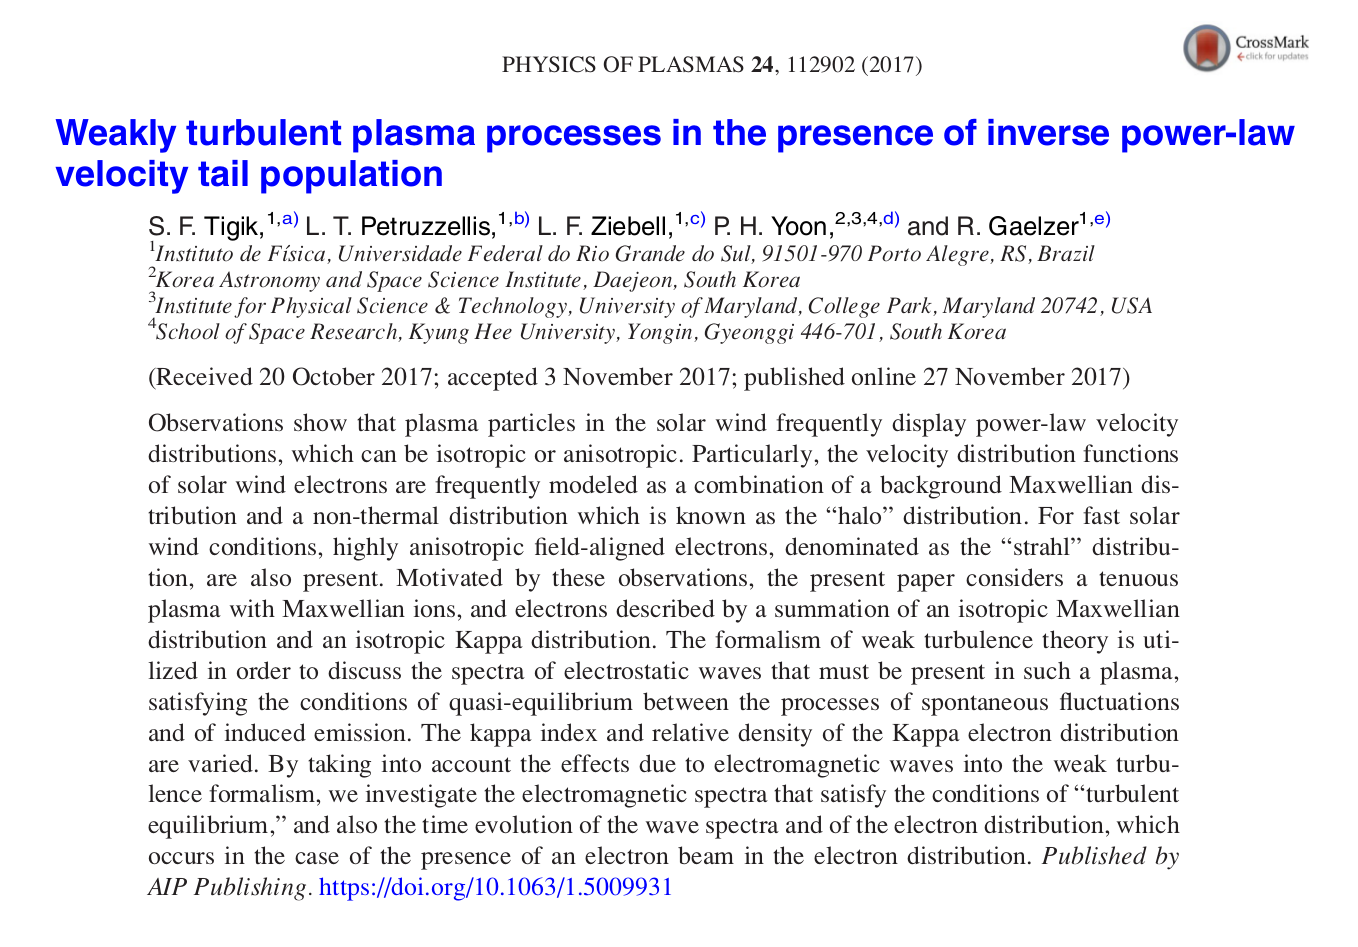
\includepdf[pages=-]{Tigik2017b.pdf}


\chapter{Applications to astrophysical plasmas}
\label{appD}
% On Earth, the plasma is considered an exotic state of matter, associated to the
% glowing gas inside fluorescent and neon lamps, microchip manufacturing, research
% laboratories, and the promise of cleaner and practically inexhaustible energy
% source once we have controlled and energetically efficient thermonuclear fusion
% \cite{bell}. Naturally occurring plasmas in our everyday life are rare, restricted
% to the occurrence of lightning during storms, flames, and the beautiful auroras
% that take place at high latitudes. In the space, however, the situation is the
% opposite. Starting in the outer layers of Earth's atmosphere, passing through the
% solar wind in the interplanetary space, to the stellar interiors and atmospheres,
% accretion disks, and molecular clouds it is estimated that something around
% $99 \sim 99.9\%$ of the observable matter in the universe is in the plasma state
% \cite{may}. So understanding the basic physics of plasma processes might help on
% interpreting and describing 

The analysis presented in this doctoral thesis has relevant contributions in the
study of the combined action of nonlinear kinetic instabilities and collisional
processes in unmagnetized, fully ionized, hydrogen plasmas. Though the plasma's
profile under consideration might be considered quite idealized, the physical
processes that are being addressed have fundamental character - the plasma waves
under consideration and the particle interactions are inherent to any plasma.
The underlying nature of these processes means that they might impact the plasma
dynamics at different astrophysical environments and also in laboratory plasmas.
Laboratory plasmas, however, are usually constrained by very specific conditions
that are unique to each experiment. This specificity makes the analysis in the
experimental context counter productive. A more broad approach was then to compare
our theoretical results with phenomena observed in the naturally occurring space
plasma\footnote{In the literature, the term ``astrophysical plasma'' is sometimes
  used to refer to the plasma observed outside the solar system, while ``space
  plasma'' is used to account for the plasma in our interplanetary space. In this
  text, however, both terms are being used as synonyms.}.


Astrophysical plasmas are observed in a vast range of densities, temperatures,
magnetic fields, ionization degree, and scale lengths\footnote{For a relatively
  brief, but comprehensive, description of the scales and characteristics of
  cosmic plasmas, see Section 1.2 of Ref. \cite{peratt2014}.}. Starting in the
outer layers of Earth's atmosphere, passing through the solar wind in the
interplanetary space, to the stellar interiors and atmospheres, accretion disks,
and molecular clouds it is estimated that something around $99 \sim 99.9\%$ of
the observable matter in the universe is in the plasma state\cite{may}. Under
cosmic conditions, even the weakly ionized gas of the neutral hydrogen regions
around galaxies or in the atmosphere of cold stars have a strong reaction to
electromagnetic fields, exhibiting the characteristic collective behavior of
plasmas\cite{tsypa,peratt2014}.
Since this ubiquity of plasmas in space came as a fact, astrophysicists and
plasma physicists have been increasingly exchanging knowledge, with plasma
physics providing theoretical background, computational and laboratory models
that might help with the interpretation and physical explanation of astrophysical
observations, and astrophysics confirming theoretical and computational
predictions on plasma physics with observations of phenomena that are unique
to space plasma\cite{tsypa,Kulsrud2005}.

On that regard, the results obtained during this graduate research can be
found on both sides of this mutual contribution. In \cite{Tigik2016a},
\cite{Tigik2016b} and \cite{Tigik2017b}, we present theoretical and
numerical evidence of plasma processes that might aid in the interpretation
and accurate modeling  of phenomena observed in the solar plasma. While in
\cite{Tigik2017a}, we introduce a new equation depicting an unknown process
and numerically analyze it in the context of solar physics; its existence
outside theory, however, will depend on the development of more advanced
space probes to be confirmed. The choice for applying our theory to
phenomena observed in the solar plasma, and not in some remote space plasma,
now became evident. The accessibility to direct, in situ measurements,
highly resolved remote sensing and high-resolution spectroscopy made the
solar plasma the right choice for our analysis.


% The absolute majority of the plasma observed in space is far away from us,
% being accessible only through analysis of the electromagnetic spectrum
% emitted from their quite remote location. A fortunate exception to this
% fact is the plasma in our solar system.





\section{Solar physics}
\label{sec:solar-physics}






The solar system is permeated with a constant plasma flow of solar origin.
This tenuous and rapid flowing plasma, know as \emph{solar wind}, is
expelled 


% The Sun is a G2 main-sequence star. From the stellar astrophysics point
% of view, it is considered ordinary, without any unique property that could
% differentiate it from other main-sequence stars; except for the fact that
% it is remarkably close to us. These two facts make the Sun a perfect model
% of study not only for several areas of astrophysics, like stellar structure
% and evolution, but also for plasma physics.





\begin{figure}[h]
  \begin{center}
    \includegraphics[width=0.48\textwidth]{corona2017.png}
    \includegraphics[width=0.4305\textwidth]{high-contrast-corona.png}
    \caption{Solar corona captured during the total solar eclipse of 2017.
      {\footnotesize Credit:}
      \href{https://hdr-astrophotography.com/high-resolution-2017-total-solar-eclipse/}
      {\footnotesize Nicolas Lefaudeux}{\footnotesize , accessed at 05/06/2019}.}
    \label{figD1}
  \end{center}
\end{figure}

\end{appendix}


\bibliographystyle{unsrturl}
\bibliography{papers,books}


\end{document}



%%% Local Variables:
%%% mode: latex
%%% TeX-master: t
%%% End:
